\pagenumbering{arabic}
%\documentclass[slides]{beamer}
\documentclass[mathserif, 10pt]{beamer}
\usepackage[framesassubsections]{beamerprosper}
\setbeamercovered{transparent}
%\documentclass[slides,hyperref={pdfpagelabels=false}]{beamer}
%\documentclass[handout,gray]{beamer}
\usepackage[T1]{fontenc}
\usepackage[utf8]{inputenc}
\usepackage{textcomp}
\usepackage{algorithm}
\usepackage{algorithmic}
\usepackage{color}
\usepackage{braket}
\usepackage{verbatim}
\usepackage{amsbsy}
\usepackage{multirow}
\usepackage{multicol}
\usepackage{booktabs} % Make some nice tables
\usepackage{ae,aecompl}

%%%%%%%%%%%% COULEURS %%%%%%%%%%%%%%%%%%%%%%%%%%%

\mode<presentation>
{
  \definecolor{beamerstructure}{RGB}{43,79,112}
  \definecolor{sidebackground}{RGB}{230,242,250}
  \definecolor{CTCC}{RGB}{133,188,228}
  \color{beamerstructure}
  \usetheme{default}
  \usepackage{courier}
  \beamertemplateballitem
\setbeamertemplate{navigation symbols}{}
%\setbeamertemplate{sidebar left}{\thispdfpagelabel{\insertframenumber}}
%\setbeamertemplate{footline}{\quad\insertframenumber}
%\usecolortheme{CTCC}
}
\usebackgroundtemplate{
\includegraphics[width=1.02\paperwidth]
{../templets/ctcc_general.jpg}}

\title{\\\vspace{1cm}
Benchmarking DFT functionals on \\ magnetic properties}
%\subtitle{\textcolor{magenta}{My subtitle (if applicable)}}
\author{Stig Rune Jensen}
\institute[CTCC]{\\[-6mm]stig.r.jensen@uit.no\\
[6mm]UiT - The Arctic University of Norway\\[6mm]

\includegraphics[height=1.5cm]{../templets/uio.pdf}\hspace{1cm} 

\includegraphics[height=1.5cm]{../templets/sff.pdf}\hspace{1cm}

\includegraphics[height=1.5cm]{../templets/uit.pdf}}
\date{CTCC meeting in Alta\\ April 7 2016}

%\newtheorem{lemma}{Proposition}
\newcommand{\fixme}[1]{{\small\em \color{red} #1 \normalsize}}

\newcommand{\unitboxd}{\ensuremath{\left[0,1\right]^d}}
\newcommand{\Exp}[1]  {\ensuremath{\cdot 10^{#1}}}
\newcommand{\etal}{{\emph{et al.}\ }}
\newcommand{\abinitio}{{\emph{ab initio }\ }}
\newcommand{\mycomment}[1]{{\large \bf #1}}
\newlength{\dch}
\newlength{\sch}
\newcommand{\ud}{\ensuremath{\,\mathrm{d}}}
\newcommand{\mydef}{\stackrel{\text{def}}{\hbox{=}}}
\newcommand{\setdch}{\settoheight{\dch}{\nscu{d}}}
\newcommand{\setsch}{\settoheight{\sch}{\nscucd{s}}}
\newcommand{\filter}[2]{\ensuremath{F_{(#1,#2)}}}
\newcommand{\ndfilter}[2]{\ensuremath{\mathcal{F}_{(#1,#2)}}}
\newcommand{\dsvec}[2]{\ensuremath{\begin{pmatrix} \rule{0mm}{\dch} d \\ \rule{0mm}{\sch} s \end{pmatrix}^{#1}_{#2}}}
\newcommand{\dsvbu}[2]{\ensuremath{\begin{pmatrix} \rule{0mm}{\dch} \nsbu{d} \\ \rule{0mm}{\sch} \nsbu{s} \end{pmatrix}^{#1}_{#2}}}
\newcommand{\dsvcu}[2]{\ensuremath{\begin{pmatrix} \rule{0mm}{\dch} \nscu{d} \\ \rule{0mm}{\sch} \nscu{s} \end{pmatrix}^{#1}_{#2}}}
\newcommand{\dsvcucd}[2]{\ensuremath{\begin{pmatrix} \rule{0mm}{\dch} \nscu{d} \\ \rule{0mm}{\sch} \nscucd{s} \end{pmatrix}^{#1}_{#2}}}
\newcommand{\nsopABCT}[2][]{\ensuremath{\begin{pmatrix} \rule{0mm}{\dch} A & B \\ \rule{0mm}{\sch} C & T\end{pmatrix}^{#2}_{#1}}}
\newcommand{\nsopABC}[1]{\ensuremath{\begin{pmatrix} \rule{0mm}{\dch} A & B \\ \rule{0mm}{\sch} C & 0\end{pmatrix}^{#1}}}
\newcommand{\mwtrans}[2]{\ensuremath{W_{#1\leftarrow #2}}}

\newcommand{\nscf}[1]{\ensuremath{\tilde{#1}}}
\newcommand{\nsabf}[1]{\ensuremath{\tilde{#1}}}
\newcommand{\nstf}[1]{\ensuremath{\hat{#1}}}

\newcommand{\nscucd}[1]{\ensuremath{\underset{\circ}{\overset{\circ}{#1}}}}
\newcommand{\nsbubd}[1]{\ensuremath{\underset{\bullet}{\overset{\bullet}{#1}}}}
\newcommand{\nscu}[1]{\ensuremath{\overset{\circ}{#1}}}
\newcommand{\nscd}[1]{\ensuremath{\underset{\circ}{#1}}}
\newcommand{\nsbu}[1]{\ensuremath{\overset{\bullet}{#1}}}
\newcommand{\nsbd}[1]{\ensuremath{\underset{\bullet}{#1}}}

\newcommand{\bds}[1]{\ensuremath{\boldsymbol{#1}}}
\newcommand{\wcoef}[3]{\ensuremath{\bds{#1}_{#2}^{#3}}}
\newcommand{\wcoefu}[3]{\ensuremath{\hat{\bds{#1}}_{#2}^{#3}}}
\newcommand{\wcoefd}[3]{\ensuremath{\check{\bds{#1}}_{#2}^{#3}}}
\newcommand{\wcoefud}[3]{\ensuremath{\tilde{\bds{#1}}_{#2}^{#3}}}
\newcommand{\wtrans}[2]{\ensuremath{W_{{\left[#1\right]}\leftarrow {\left[#2\right]}}}}
\newcommand{\scaling}{\phi}
\newcommand{\wavelet}{\psi}
\newcommand{\scalwav}{\varphi}
\newcommand{\scalingnd}{\phi}
\newcommand{\waveletnd}{\psi}
\newcommand{\scalwavnd}{\varphi}

\newcommand{\mycite}[1]{\cite{#1}}

\newcommand{\bs}[1]{\ensuremath{\boldsymbol #1}}
\newcommand{\Wavefunction}{\ensuremath{\Psi}}
\newcommand{\wavefunction}{\ensuremath{\psi}}

\newcommand{\orbital}{\ensuremath{\varphi}}
\newcommand{\density}{\ensuremath{\hat{\rho}}}
\newcommand{\nuclear}{\ensuremath{\hat{V}_{nuc}}}
\newcommand{\coulomb}{\ensuremath{\hat{J}}}
\newcommand{\xc}{\ensuremath{\hat{V}_{xc}}}
\newcommand{\exchange}{\ensuremath{\hat{K}}}
\newcommand{\potential}{\ensuremath{\hat{V}}}
\newcommand{\kinetic}{\ensuremath{\hat{T}}}
\newcommand{\perturbation}{\ensuremath{\hat{h}}}
\newcommand{\effPot}{\ensuremath{v_{eff}}}
\newcommand{\nucPot}{\ensuremath{v_{nuc}}}
\newcommand{\elPot}{\ensuremath{v_{el}}}
\newcommand{\xcPot}{\ensuremath{v_{xc}}}
\newcommand{\fockMat}{\ensuremath{F}}
\newcommand{\fockOper}{\ensuremath{\hat{F}}}
\newcommand{\poisson}{\ensuremath{P(r-r')}}
\newcommand{\Poisson}[1]{\ensuremath{\hat{P}\Big[#1\Big]}}
\newcommand{\helmholtz}{\ensuremath{G^{\mu}(r-r')}}
\newcommand{\Helmholtz}[1]{\ensuremath{\hat{G}_i\left[#1\right]}}
\newcommand{\Helmholtzp}[1]{\ensuremath{\hat{G}_i^{(+)}\bigg[#1\bigg]}}
\newcommand{\Helmholtzm}[1]{\ensuremath{\hat{G}_i^{(-)}\bigg[#1\bigg]}}
\newcommand{\Helm}{\ensuremath{\hat{G}}}
\newcommand{\hamiltonian}{\ensuremath{\hat{h}}}

\newcommand{\pert}[2]{\ensuremath{#1^{(#2)}}}
\newcommand{\HopB}{\ensuremath{\pert{\hat{\boldsymbol{h}}}{B}}}
\newcommand{\HopM}{\ensuremath{\pert{\hat{\boldsymbol{h}}}{M_K}}}
\newcommand{\HopBB}{\ensuremath{\pert{\hat{\boldsymbol{h}}}{B,B}}}
\newcommand{\HopMB}{\ensuremath{\pert{\hat{\boldsymbol{h}}}{M_K,B}}}
\newcommand{\HmatB}{\ensuremath{\pert{\boldsymbol{h}}{B}}}
\newcommand{\HmatM}{\ensuremath{\pert{\boldsymbol{h}}{M_K}}}
\newcommand{\HmatBB}{\ensuremath{\pert{\boldsymbol{h}}{B,B}}}
\newcommand{\HmatMB}{\ensuremath{\pert{\boldsymbol{h}}{M_K,B}}}

\newcommand{\gb}[1]{green!#1!black}
\newcommand{\rb}[1]{red!#1!black}
\newcommand{\bb}[1]{blue!#1!black}
\newcommand{\coleq}{red!60!black}
\newcommand{\du}{\textrm{d}}

\newcommand{\Node}{\texttt{Node\ }}
\newcommand{\node}{\texttt{node\ }}
\newcommand{\nodes}{\texttt{nodes\ }}
\newcommand{\Tree}{\texttt{Tree\ }}
\newcommand{\tree}{\texttt{tree\ }}
\newcommand{\trees}{\texttt{trees\ }}


\begin{document}

\footnotesize
\setlength{\unitlength}{\textwidth}

{
\usebackgroundtemplate{
\includegraphics[width=1.02\paperwidth]
{../templets/ctcc_forside.jpg}}
\maketitle
}

%\begin{frame}
    \frametitle{Summary}
    About the presented computer codes
    \begin{itemize}
        \item   written in C++
        \item   parallelized using OpenMP, MPI and hybrid
        \item   based on \textbf{multiresolution analysis} and the \textbf{multiwavelet basis}
    \end{itemize}
    \ \\
    \ \\
    \pause
    Features of \textbf{MultiResolution Computation Program Package (MRCPP)}
    \begin{itemize}
        \item   Multiresolution representations of functions and operators
        \item   On-the-fly adaptive multiresolution grids
        \item   Arithmetic operations and numerical integrals
        \item   \textbf{Linear scaling} application of operators
        \item   \textbf{Guaranteed accuracy}
    \end{itemize}
    \ \\
    \ \\
    %\pause
    %Features of \textbf{MultiResolution Grid (MRGrid)}
    %\begin{itemize}
    %    \item   Numerical grid generator for conventional QM programs
    %    \item   Provide accurate and reliable numerical grids for diffuse properties
    %\end{itemize}
    %\ \\
    %\ \\
    \pause
    Features of \textbf{MultiResolution Chemistry (MRChem)}
    \begin{itemize}
        \item   Numerical solution for the electronic structure of molecules
        \item   SCF level of theory (Hartree-Fock and DFT)
        \item   Spin-restricted and spin-unrestricted calculations
        \item   Able to attain high (guaranteed) accuracy in energies
	\item	Electric and magnetic linear response properties
    \end{itemize}
\end{frame}


%\begin{frame}
    \frametitle{Outlook}
    \begin{itemize}
        \item   \textbf{Paper I}
        \begin{itemize}
            \item   Multiwavelets
            \item   Function representations
            \item   Varying polynomial order
        \end{itemize}
        \ \\
        \ \\
        \item   \textbf{Paper II}
        \begin{itemize}
            \item   Operator representation
            \item   Parallel implementation
            \item   Coulomb interaction
        \end{itemize}
        \ \\
        \ \\
        \item   \textbf{Paper III}
        \begin{itemize}
            \item   Density Functional Theory
            \item   Integral formulation
            \item   Iterative algorithm
        \end{itemize}
    \end{itemize}
\end{frame}

\begin{frame}
\frametitle{Introduction}
\centering

\begin{columns}
\begin{column}[b]{0.5\textwidth}
    \begin{itemize}
        \item   Wavelet theory
        \item   Abel price
        \item   BigDFT
        \item   MADNESS
    \end{itemize}
\end{column}
\begin{column}[b]{0.5\textwidth}
    \begin{itemize}
        \item   Signal processing
        \item   Image compression
        \item   Gravitational waves
        \item   JPEG2000
        \item   MP3
    \end{itemize}
\end{column}
\end{columns}
\end{frame}

%\begin{frame}
%    \centering
%    \Large{Part I:}\\
%    \ \\
%    \ \\
%    \centering
%    \Large{Adaptive order polynomial algorithm in a\\
%            multiwavelet representation scheme}
%\end{frame}


%\begin{frame}
%\frametitle{Multiwavelets}
%\begin{columns}
%\begin{column}[b]{0.55\linewidth}
%\begin{itemize}
%    \item   \textbf{Scaling functions} are polynomials or order $\leq k$\\
%	    on the unit interval
%    \item   \textbf{Dilation and translation} to refinement scale $n$
%	    \begin{equation}
%		\nonumber
%		\phi_l^n(x) = 2^{n/2}\phi(2^nx-l)
%	    \end{equation}
%    \item   At scale $n$ there are $2^n$ subintervals
%    \item   The length of each subinterval is $2^{-n}$
%    \item   \textbf{Scaling projection} at scale $N$
%	    \begin{equation}
%		\nonumber
%		f(x) \approx f^N(x) = \sum_l s_l^N \phi_l^N(x)
%	    \end{equation}
%	    \ \\
%	    \ \\
%    \item   For a $k$-order basis in $d$ dimensions there are\\
%	    $\left(2(k+1)\right)^{nd}$ basis functions at scale $n$\\
%\end{itemize}
%\centering
%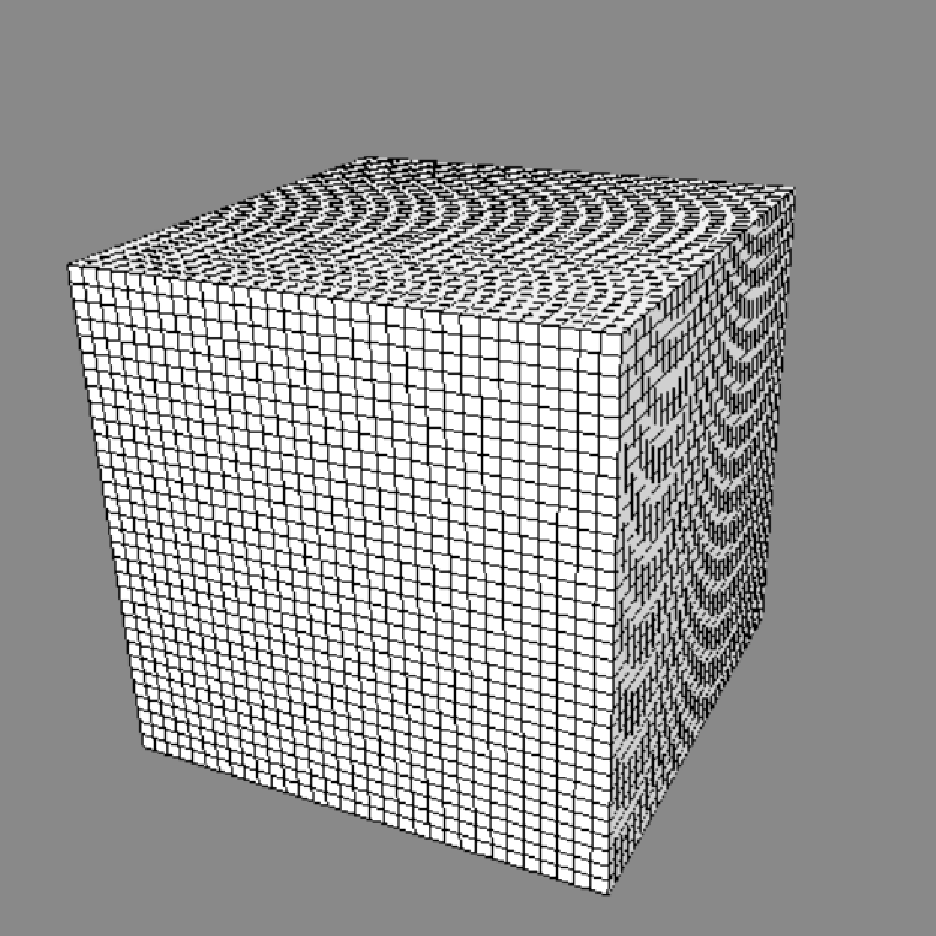
\includegraphics[scale=0.2]{figures/unifgrid.pdf}
%\end{column}
%
%\begin{column}[b]{0.45\linewidth}
%\centering
%\includegraphics[scale=0.3, clip, viewport=150 450 450 750]
%    {figures/scaling.pdf}\\
%\includegraphics[scale=0.3, clip, viewport=100 400 500 800]
%    {figures/refinement.pdf}
%\end{column}
%
%\end{columns}
%\end{frame}

\begin{frame}
\frametitle{Multiwavelets}
\centering
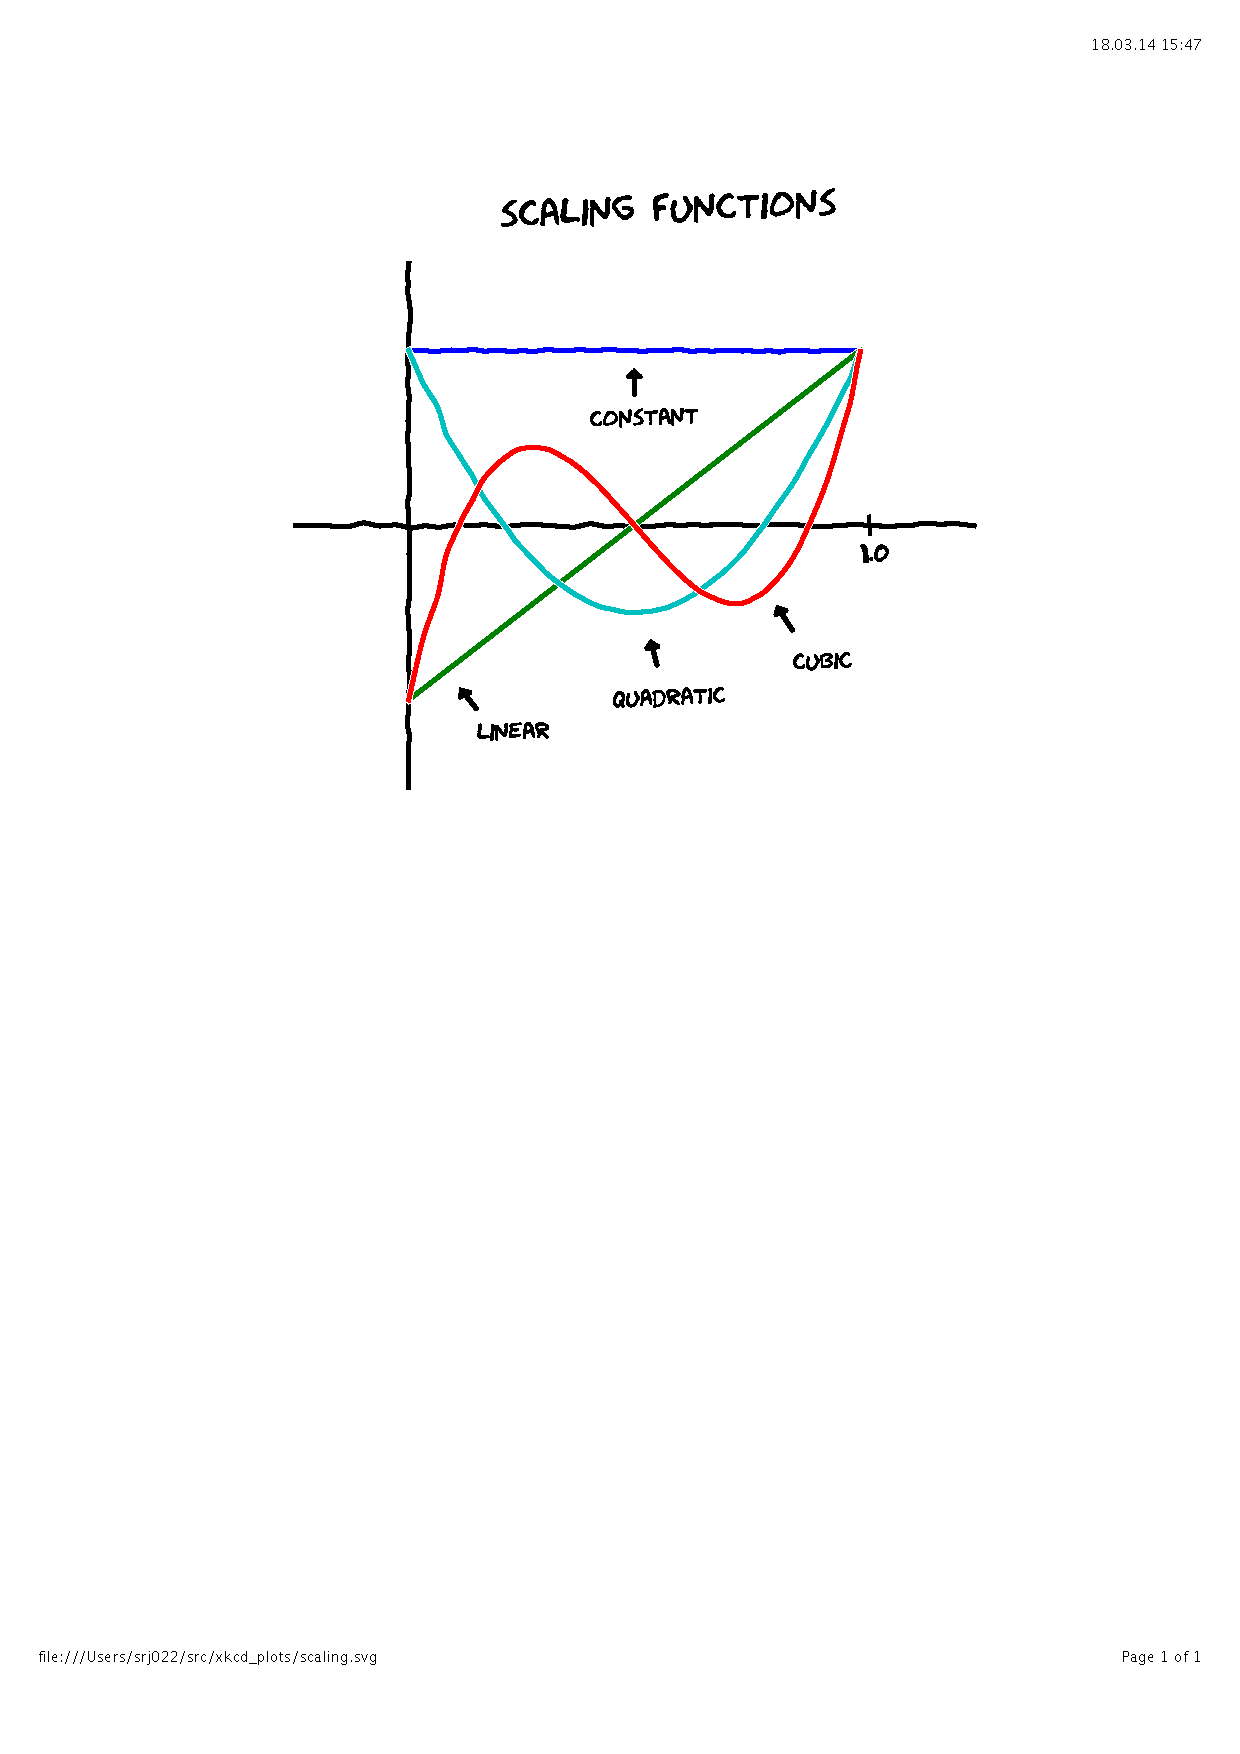
\includegraphics[scale=0.5, clip, viewport=150 450 450 750]{figures/scaling.pdf}
\end{frame}

%\begin{frame}
%\frametitle{Multiwavelets}
%\centering
%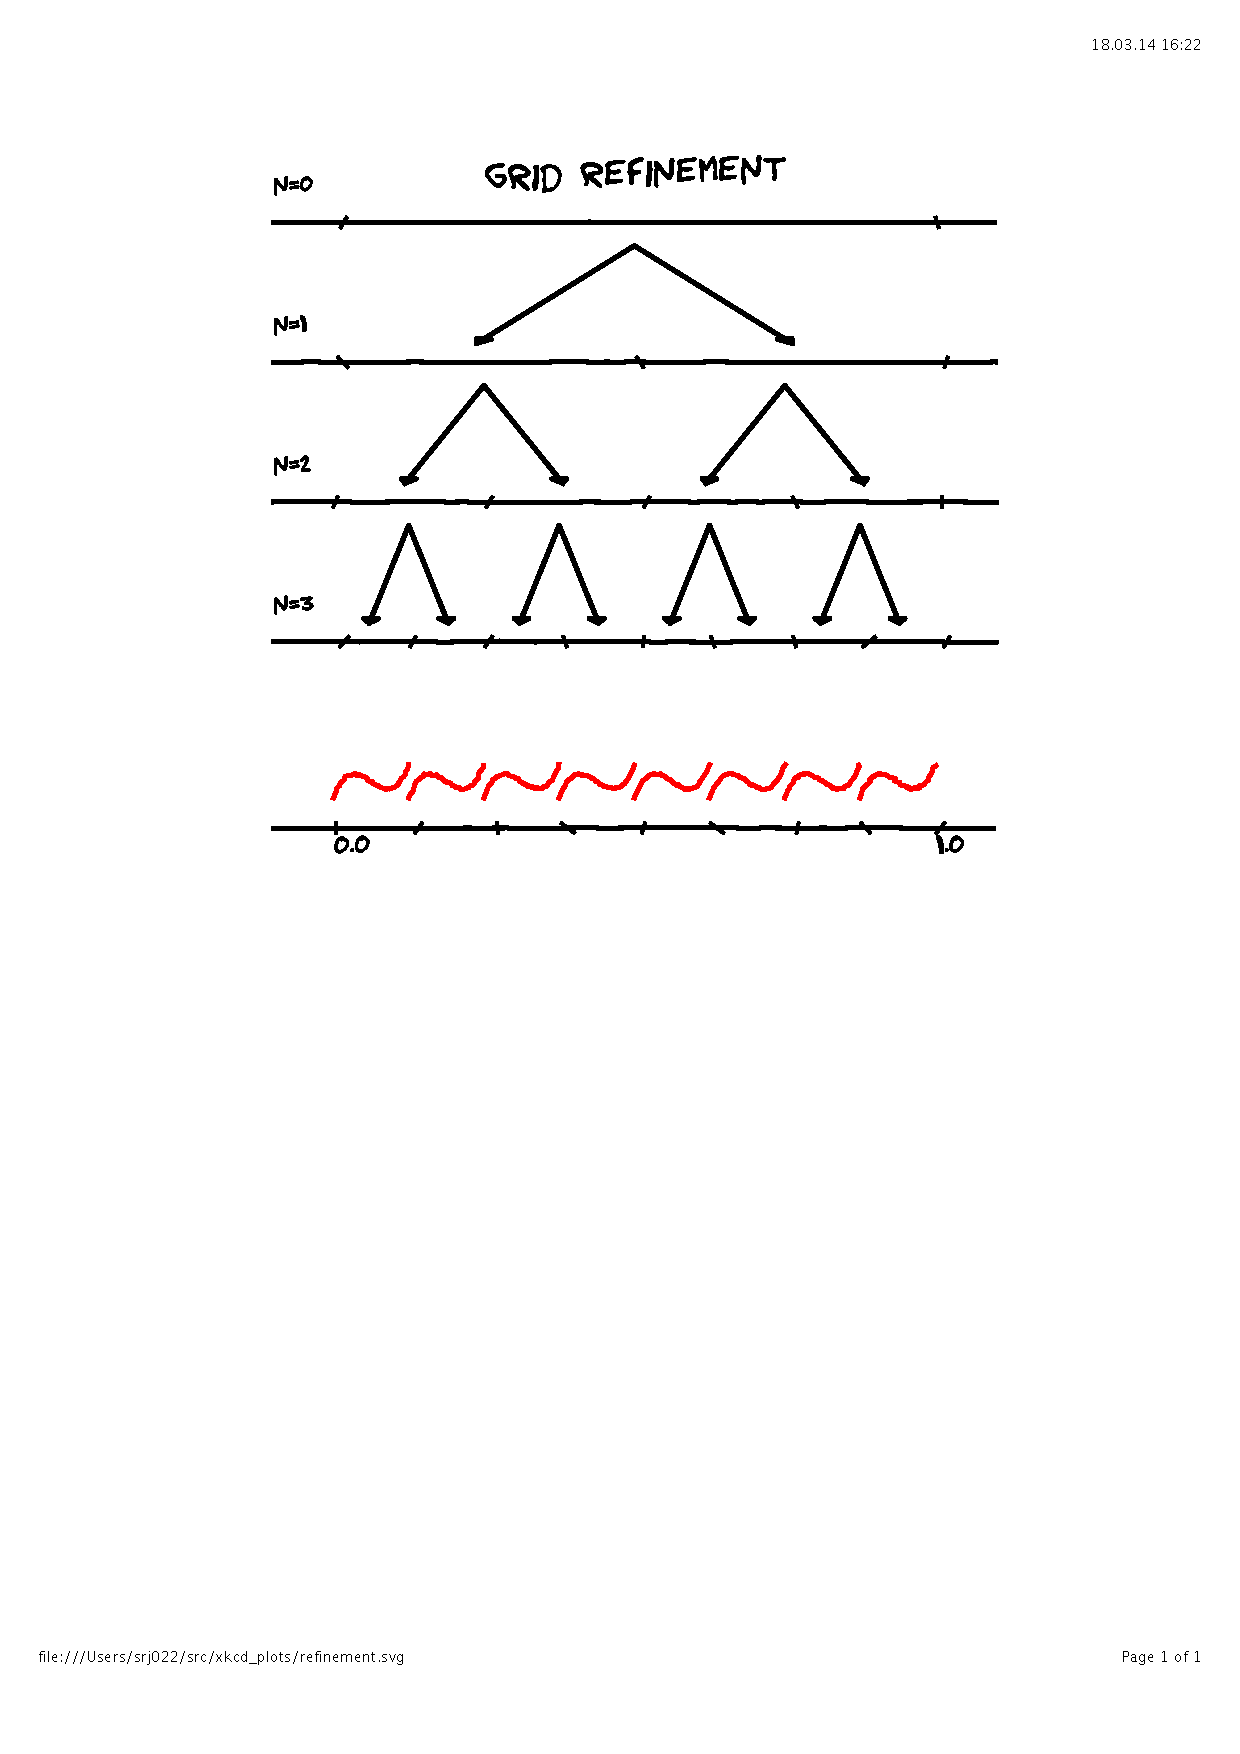
\includegraphics[scale=0.5, clip, viewport=100 400 500 800]{figures/refinement.pdf}
%\end{frame}

%\begin{frame}
%\frametitle{Multiwavelets}
%\centering
%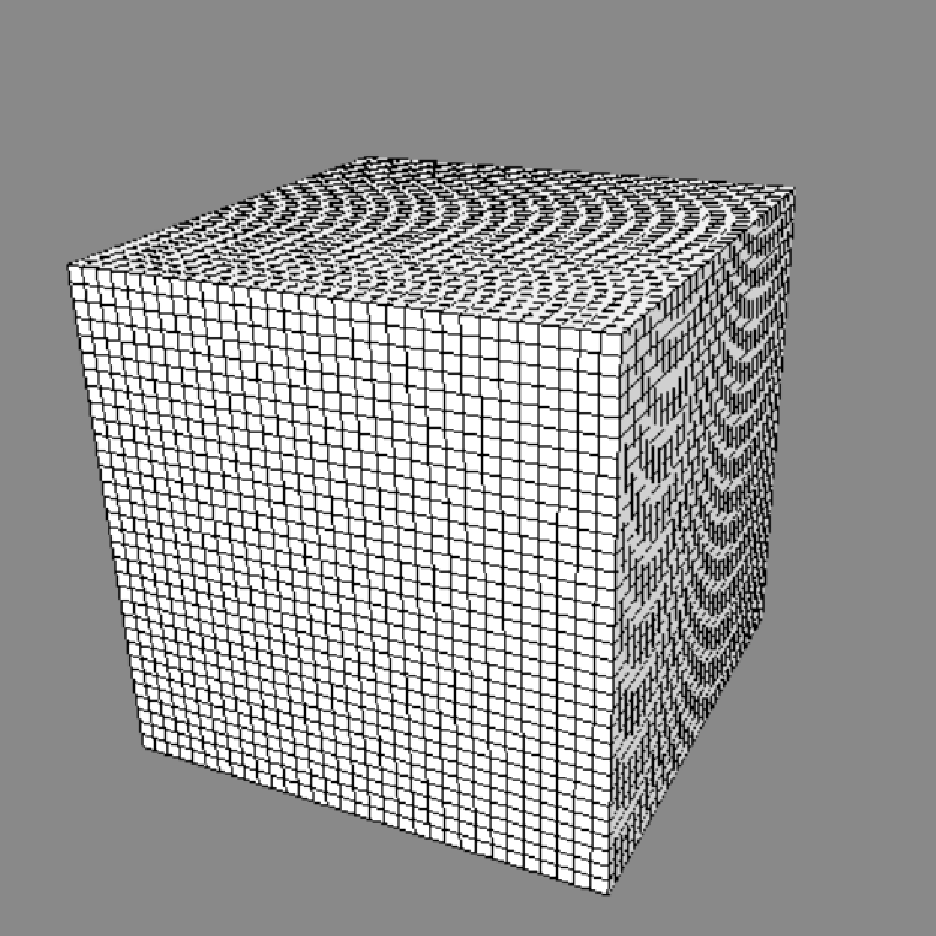
\includegraphics[scale=0.35]{figures/unifgrid.pdf}
%\end{frame}

\begin{frame}
\frametitle{Multiwavelets}
\centering
\only<1>{\ \ \ 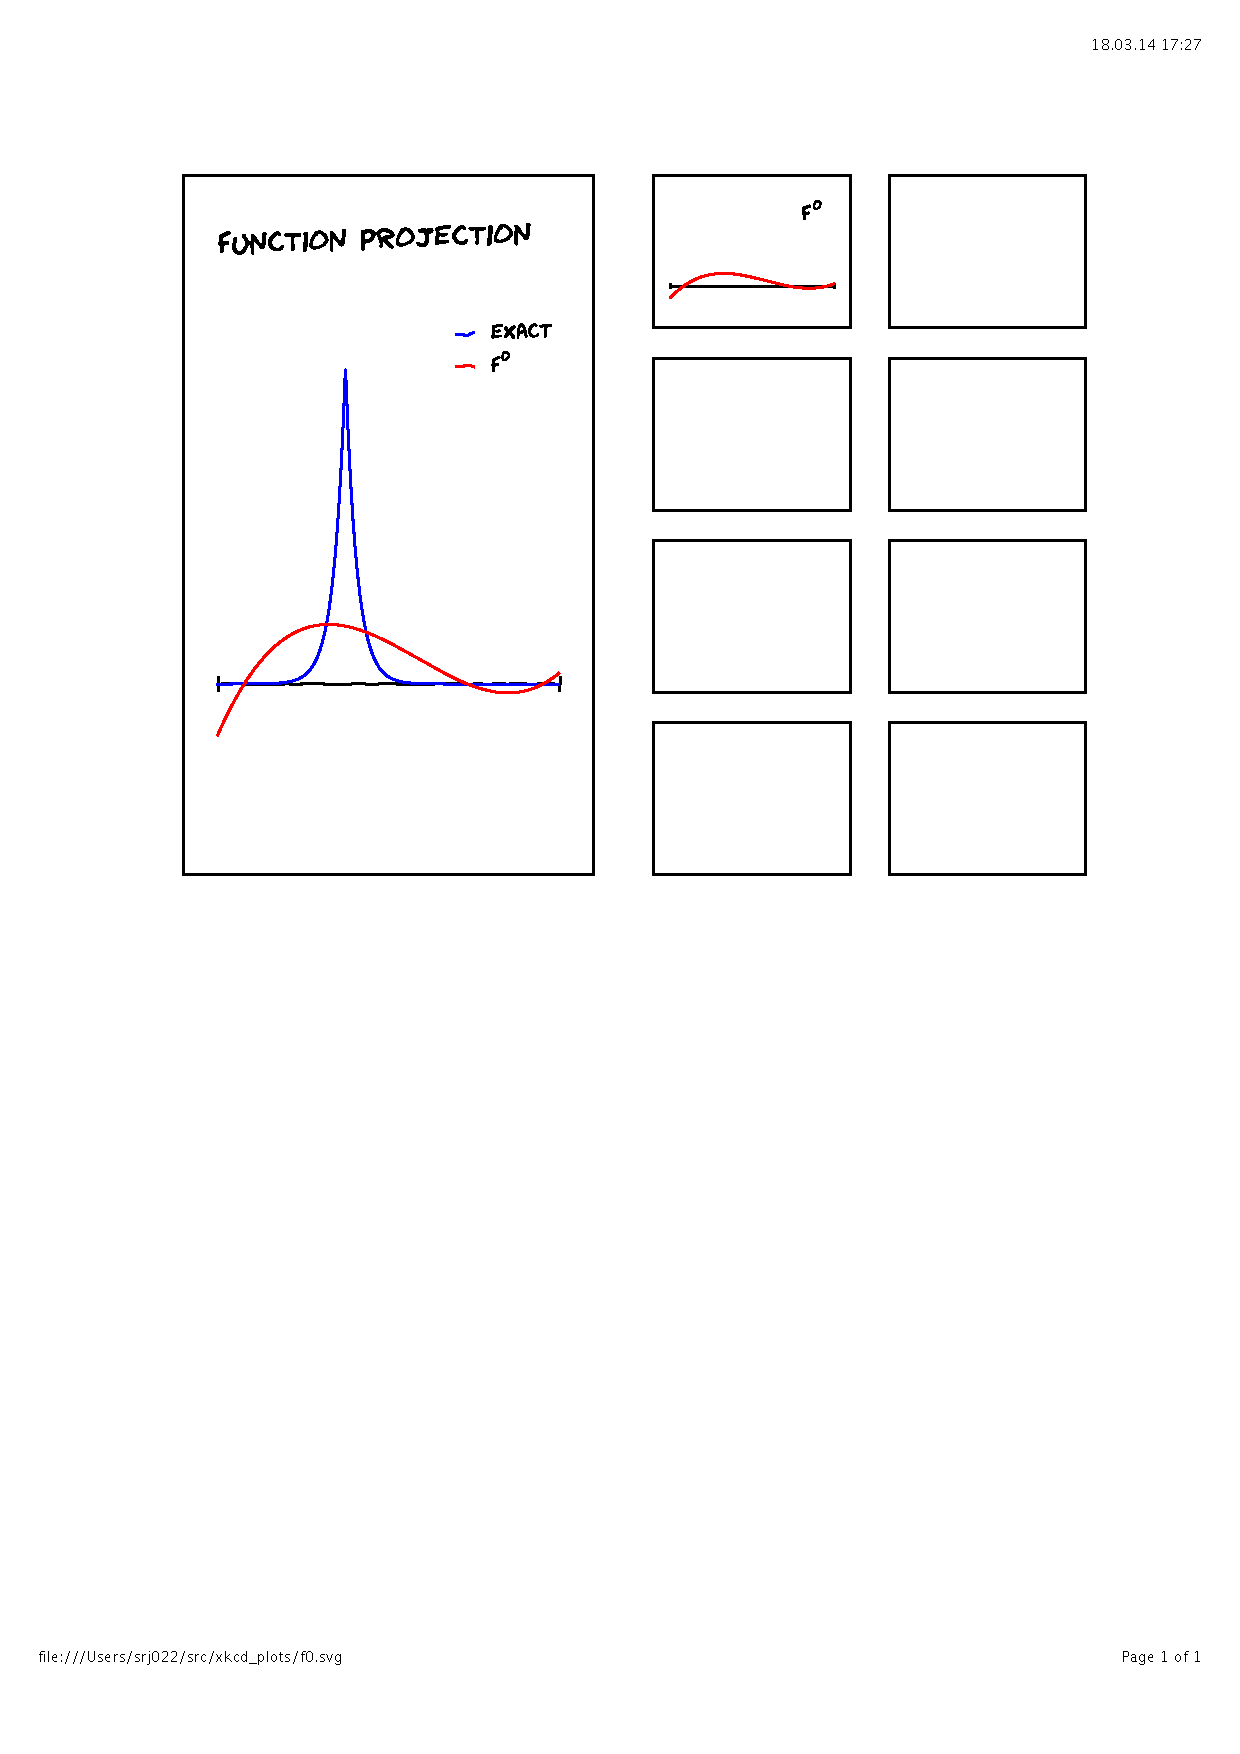
\includegraphics[clip, viewport=50 100 600 800, scale=0.5]
    {figures/f0.pdf}}
\only<2>{\ \ 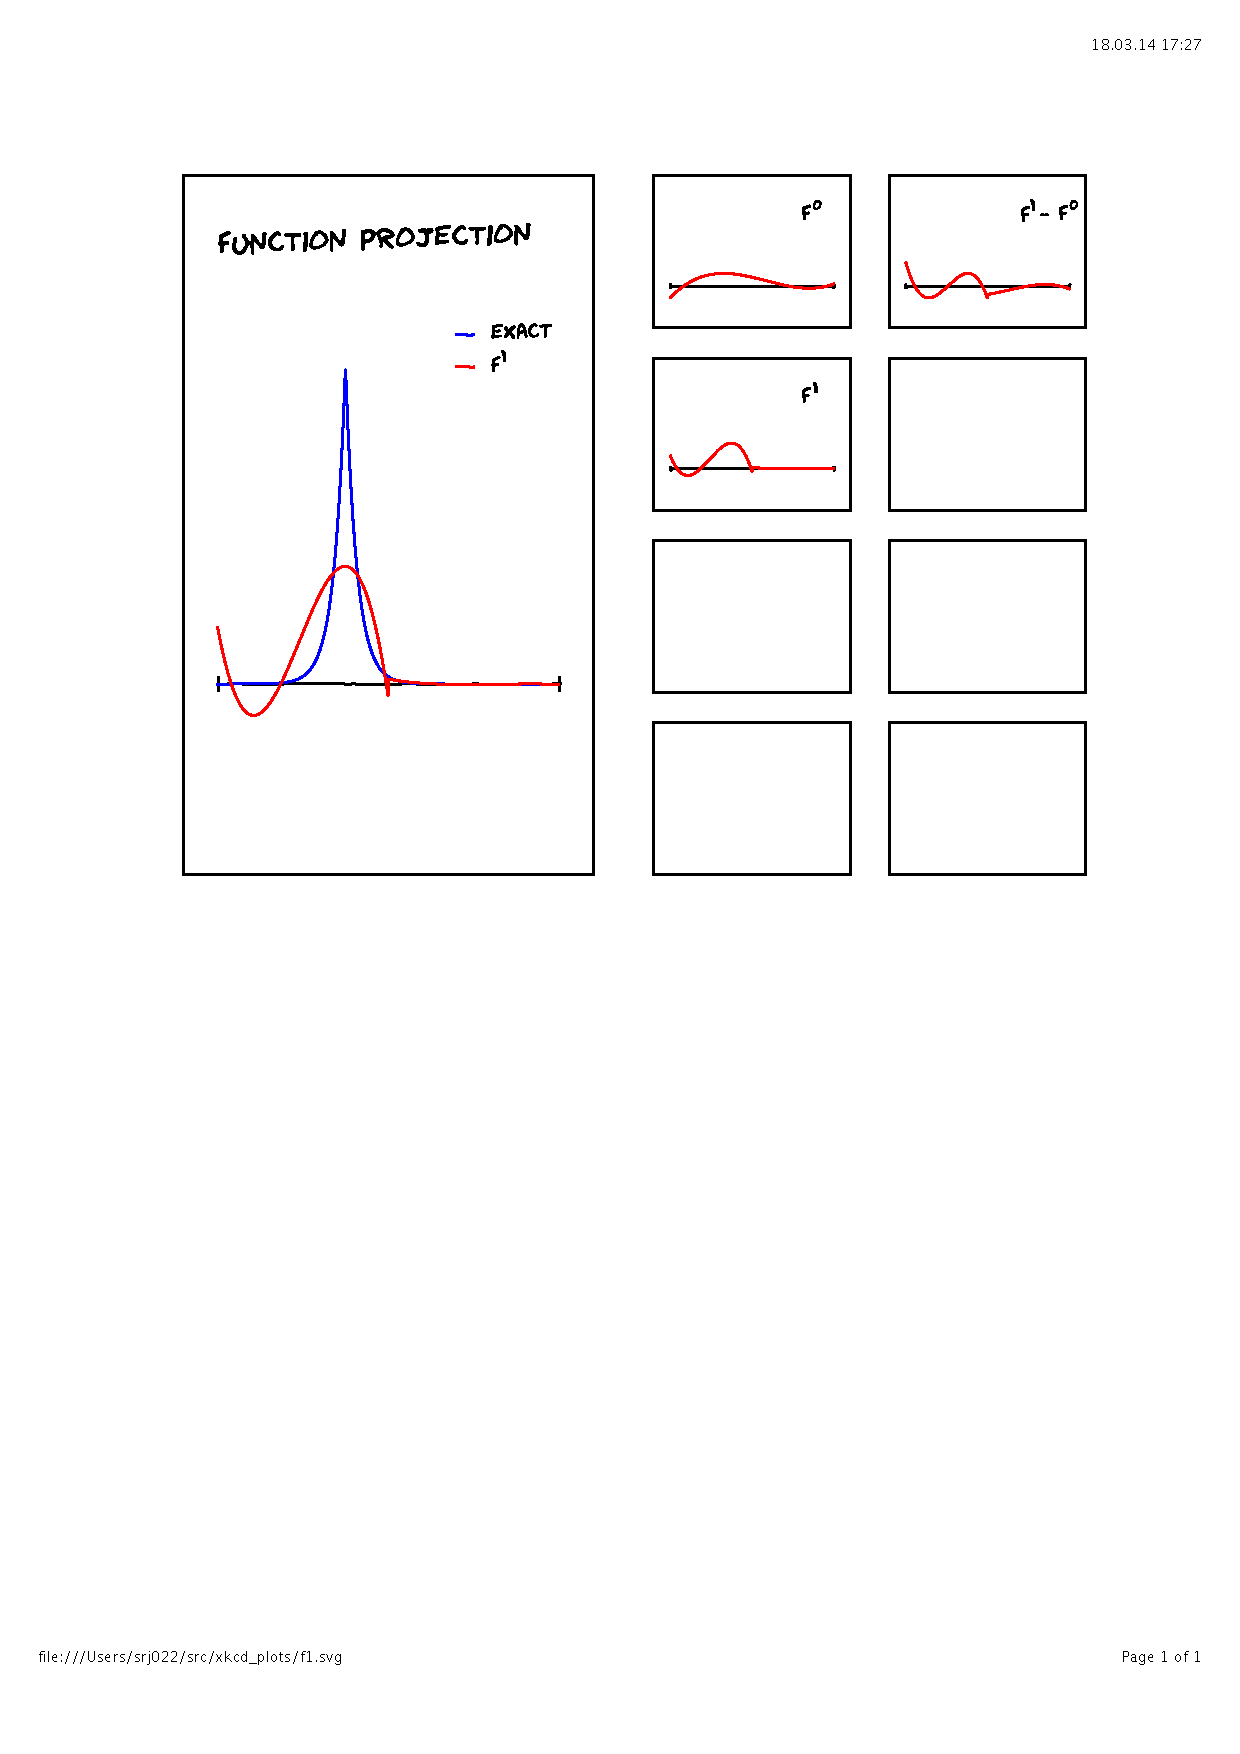
\includegraphics[clip, viewport=50 100 600 800, scale=0.5]
    {figures/f1.pdf}}
\only<3>{\ 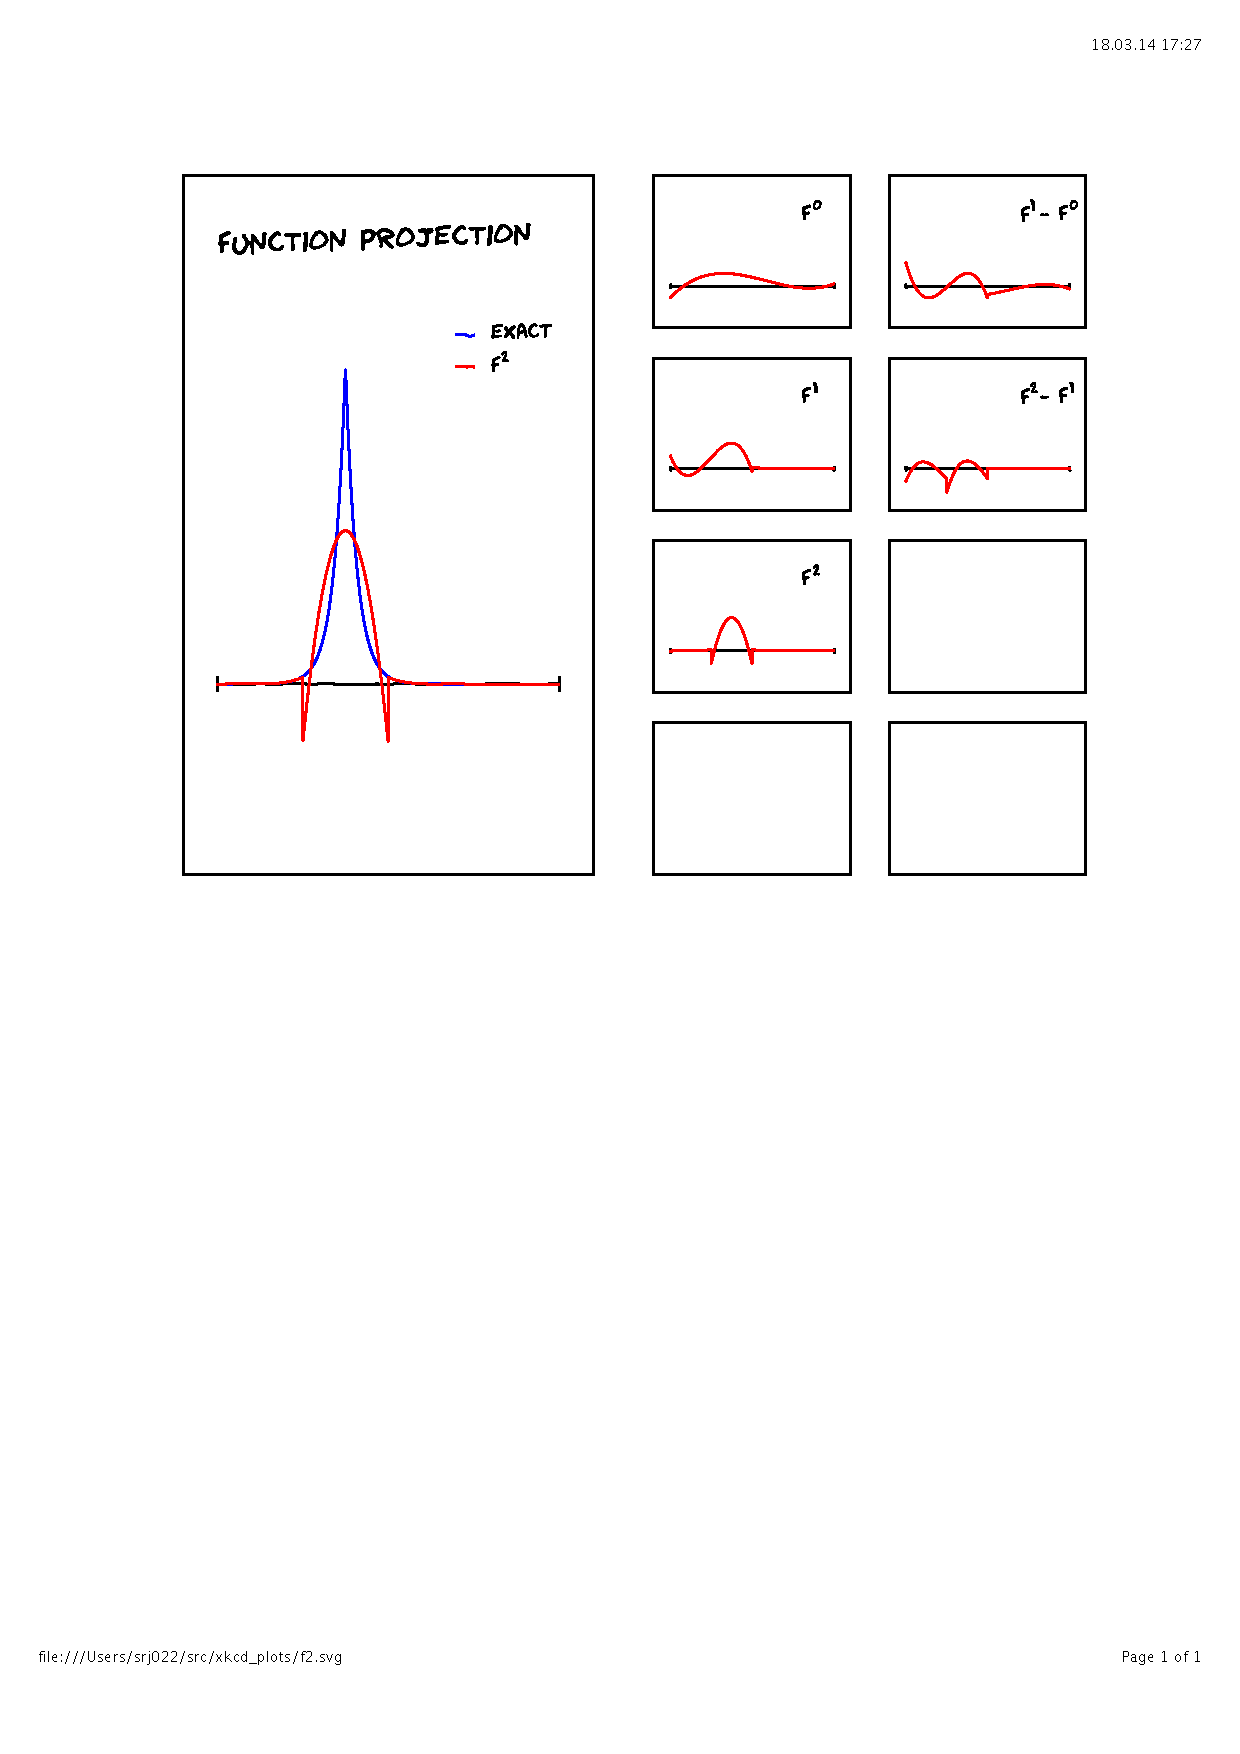
\includegraphics[clip, viewport=50 100 600 800, scale=0.5]
    {figures/f2.pdf}}
\only<4>{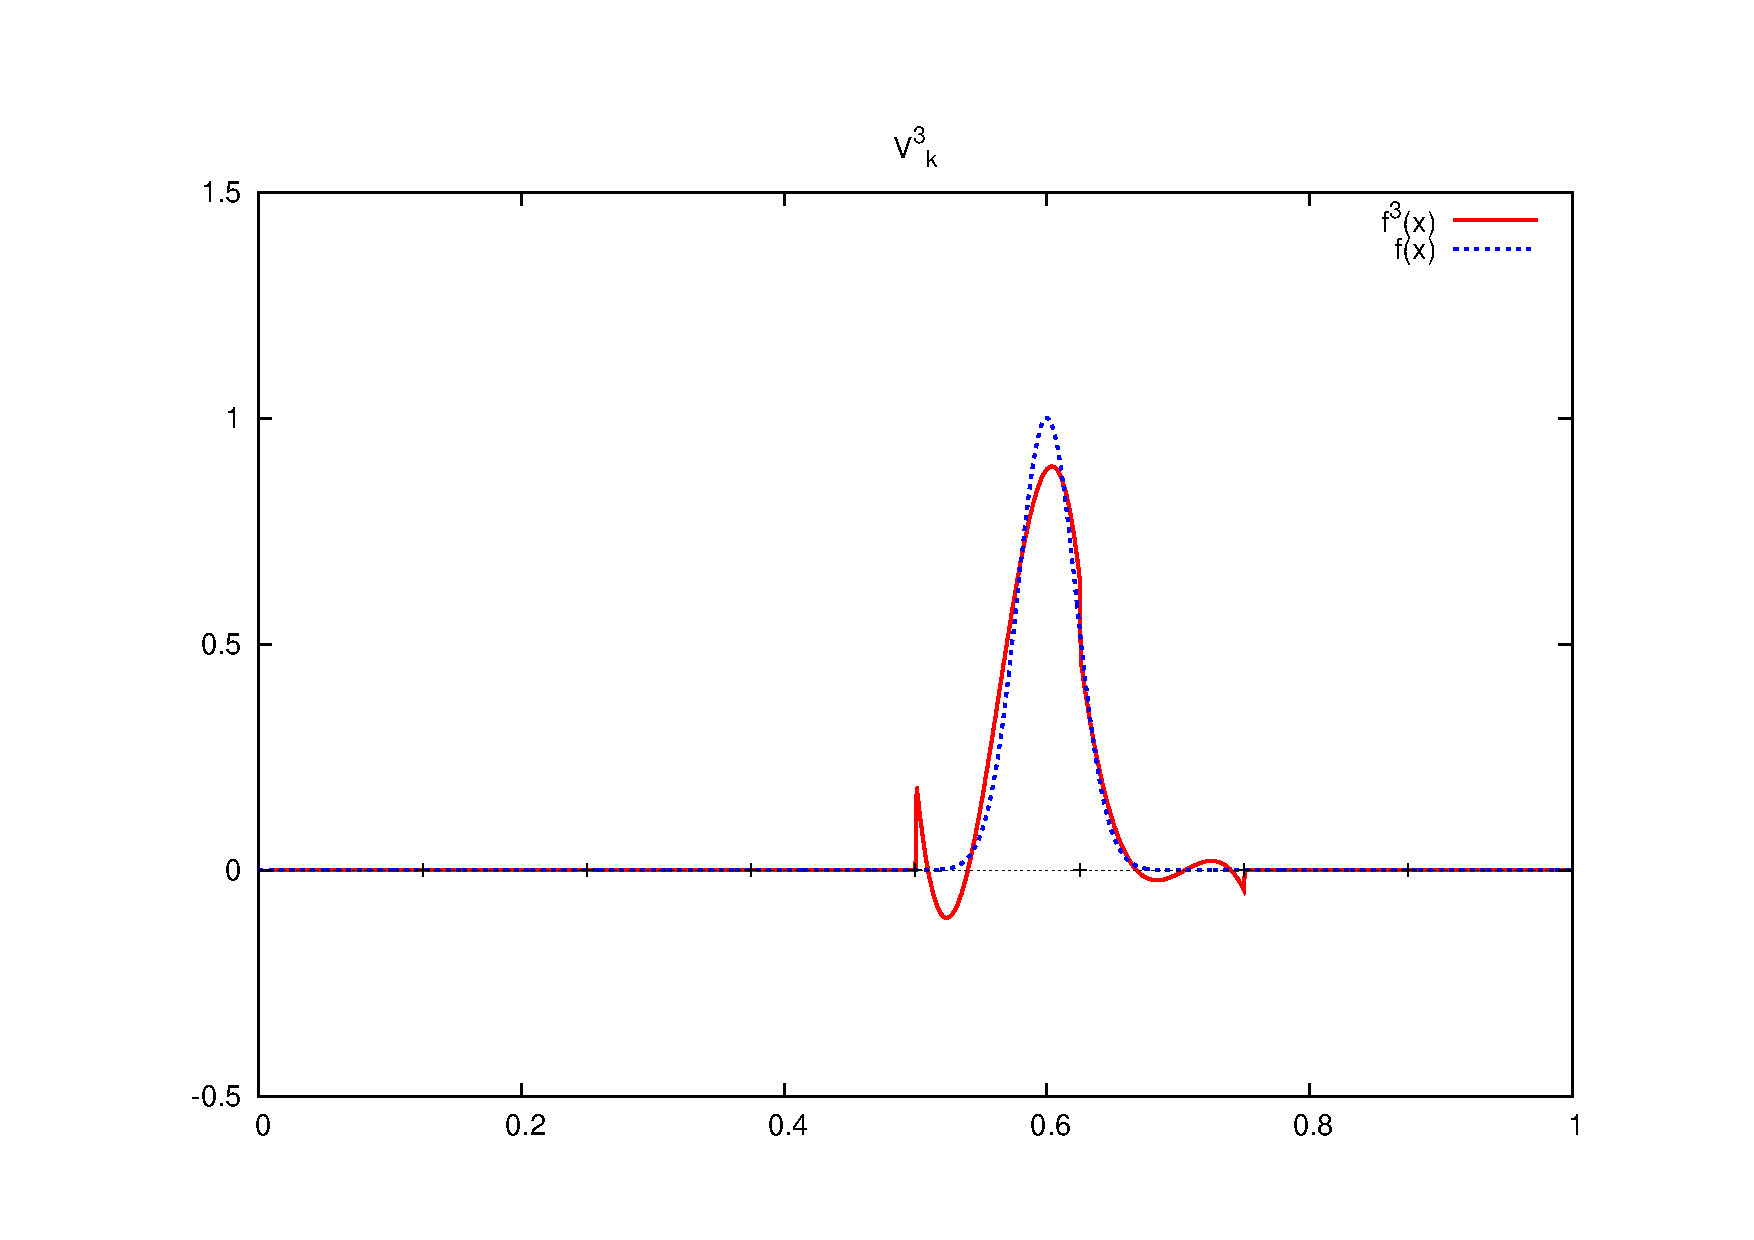
\includegraphics[clip, viewport=50 100 600 800, scale=0.5]
    {figures/f3.pdf}}
\only<5>{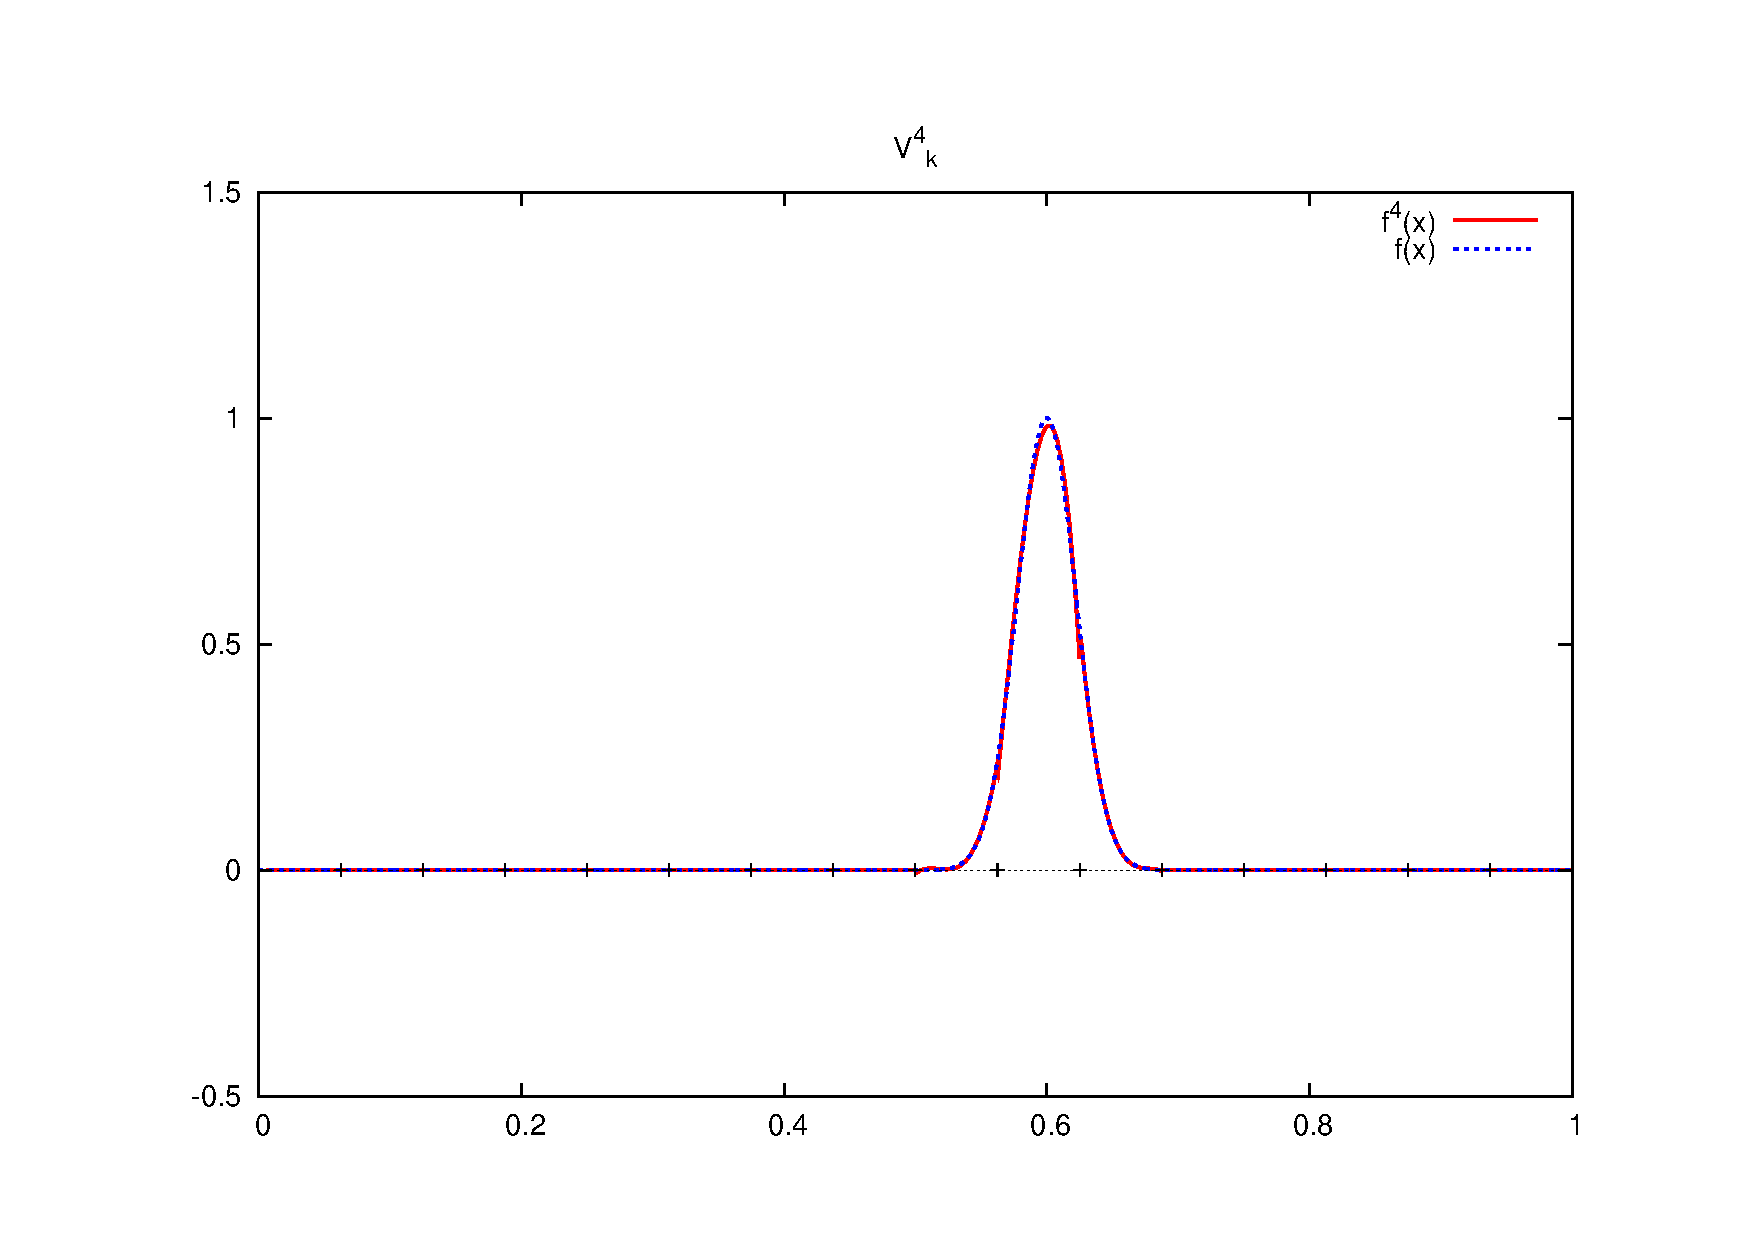
\includegraphics[clip, viewport=50 100 600 800, scale=0.5]
    {figures/f4.pdf}}
\end{frame}

%\begin{frame}
%\frametitle{Multiwavelets}
%\centering
%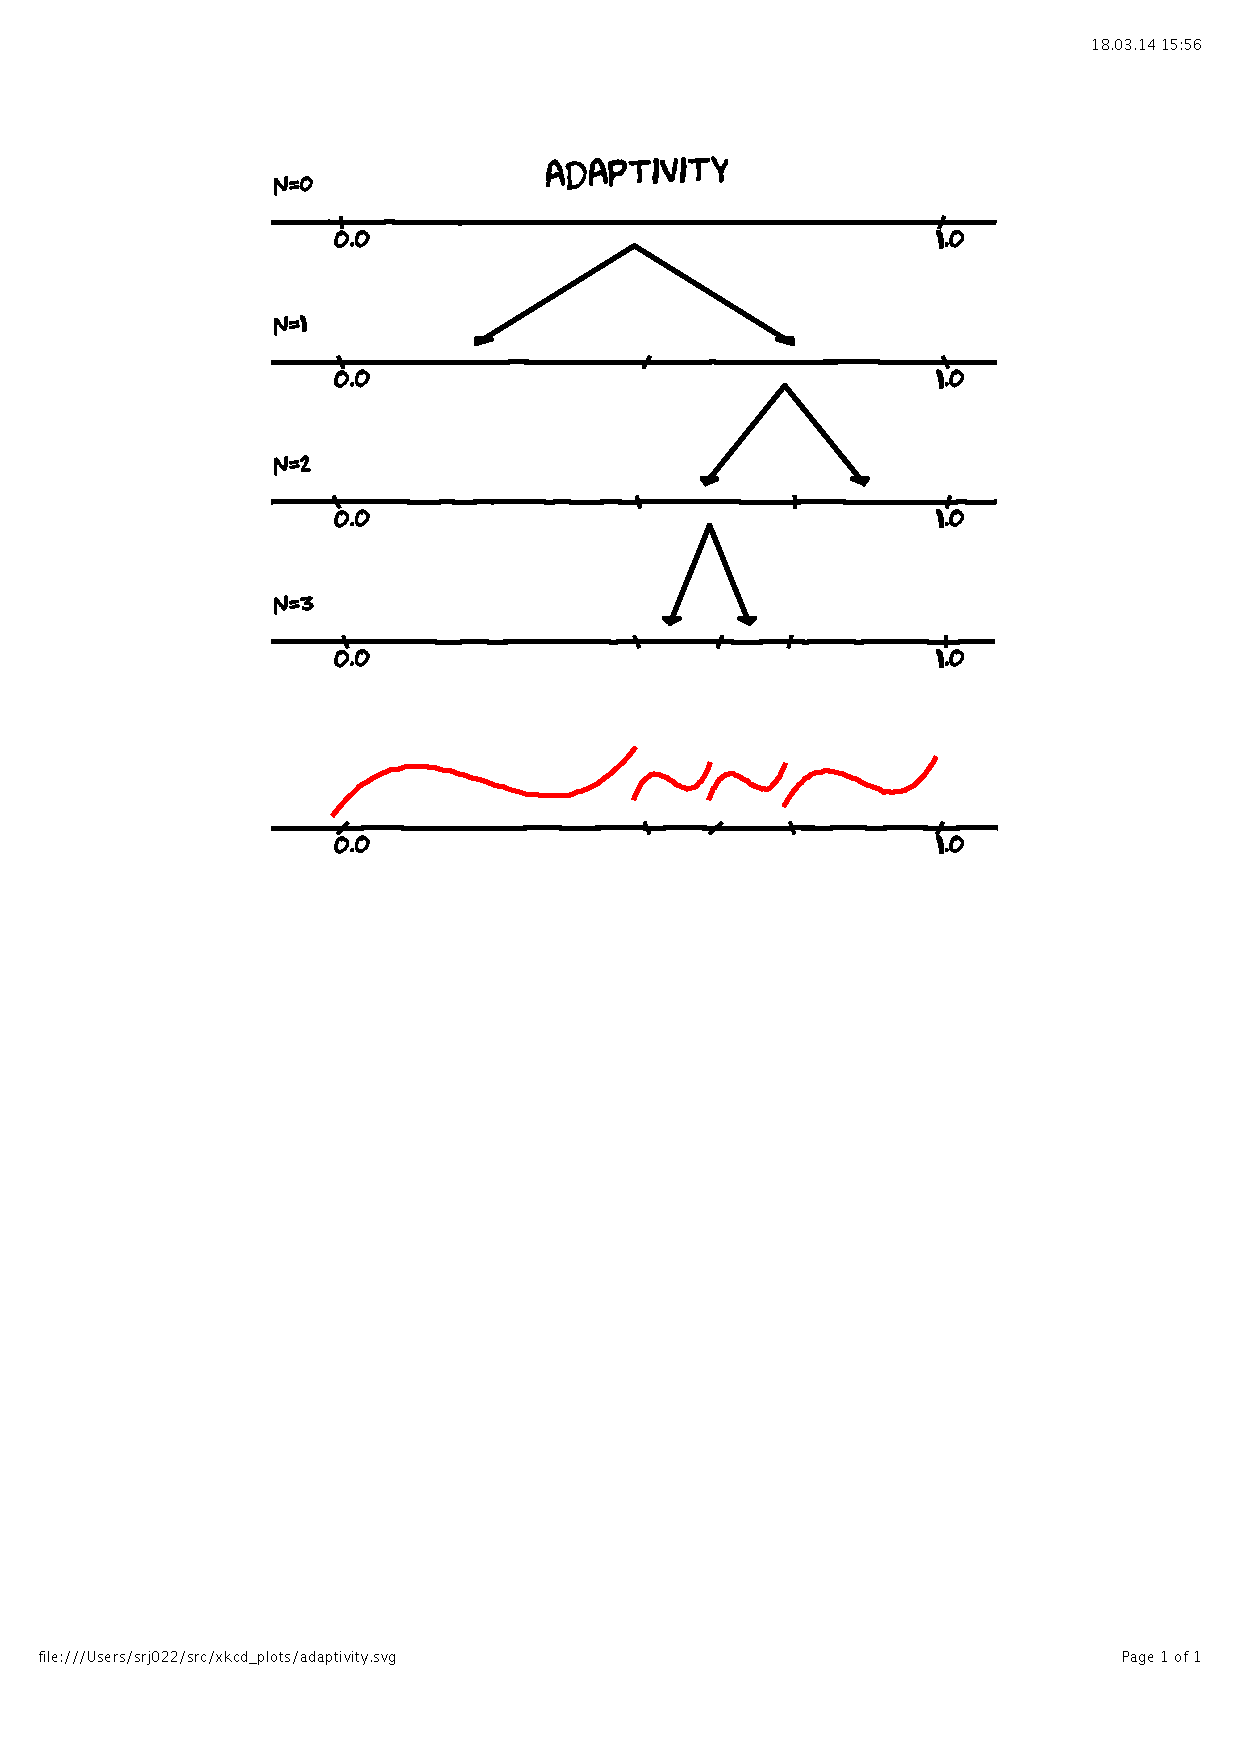
\includegraphics[scale=0.5, clip, viewport=100 400 500 800]{figures/adaptivity.pdf}
%\end{frame}

\begin{frame}
\frametitle{Multiwavelets}
\centering
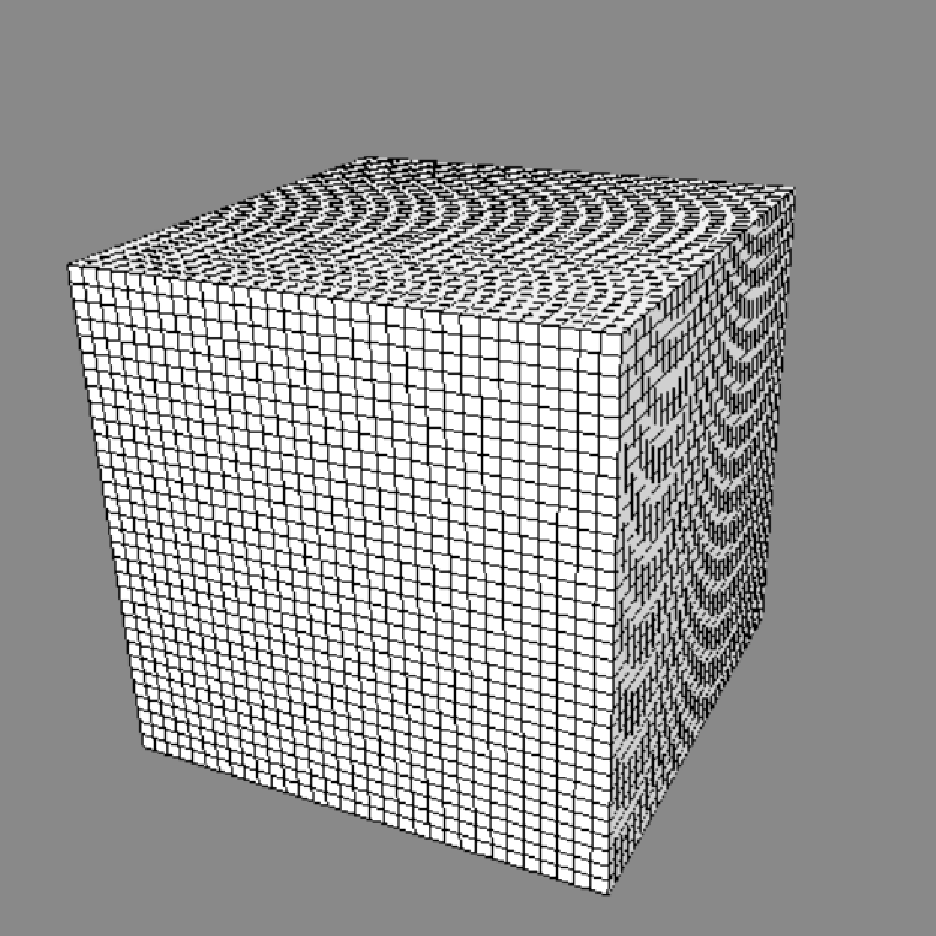
\includegraphics[scale=0.3]{figures/unifgrid.pdf}
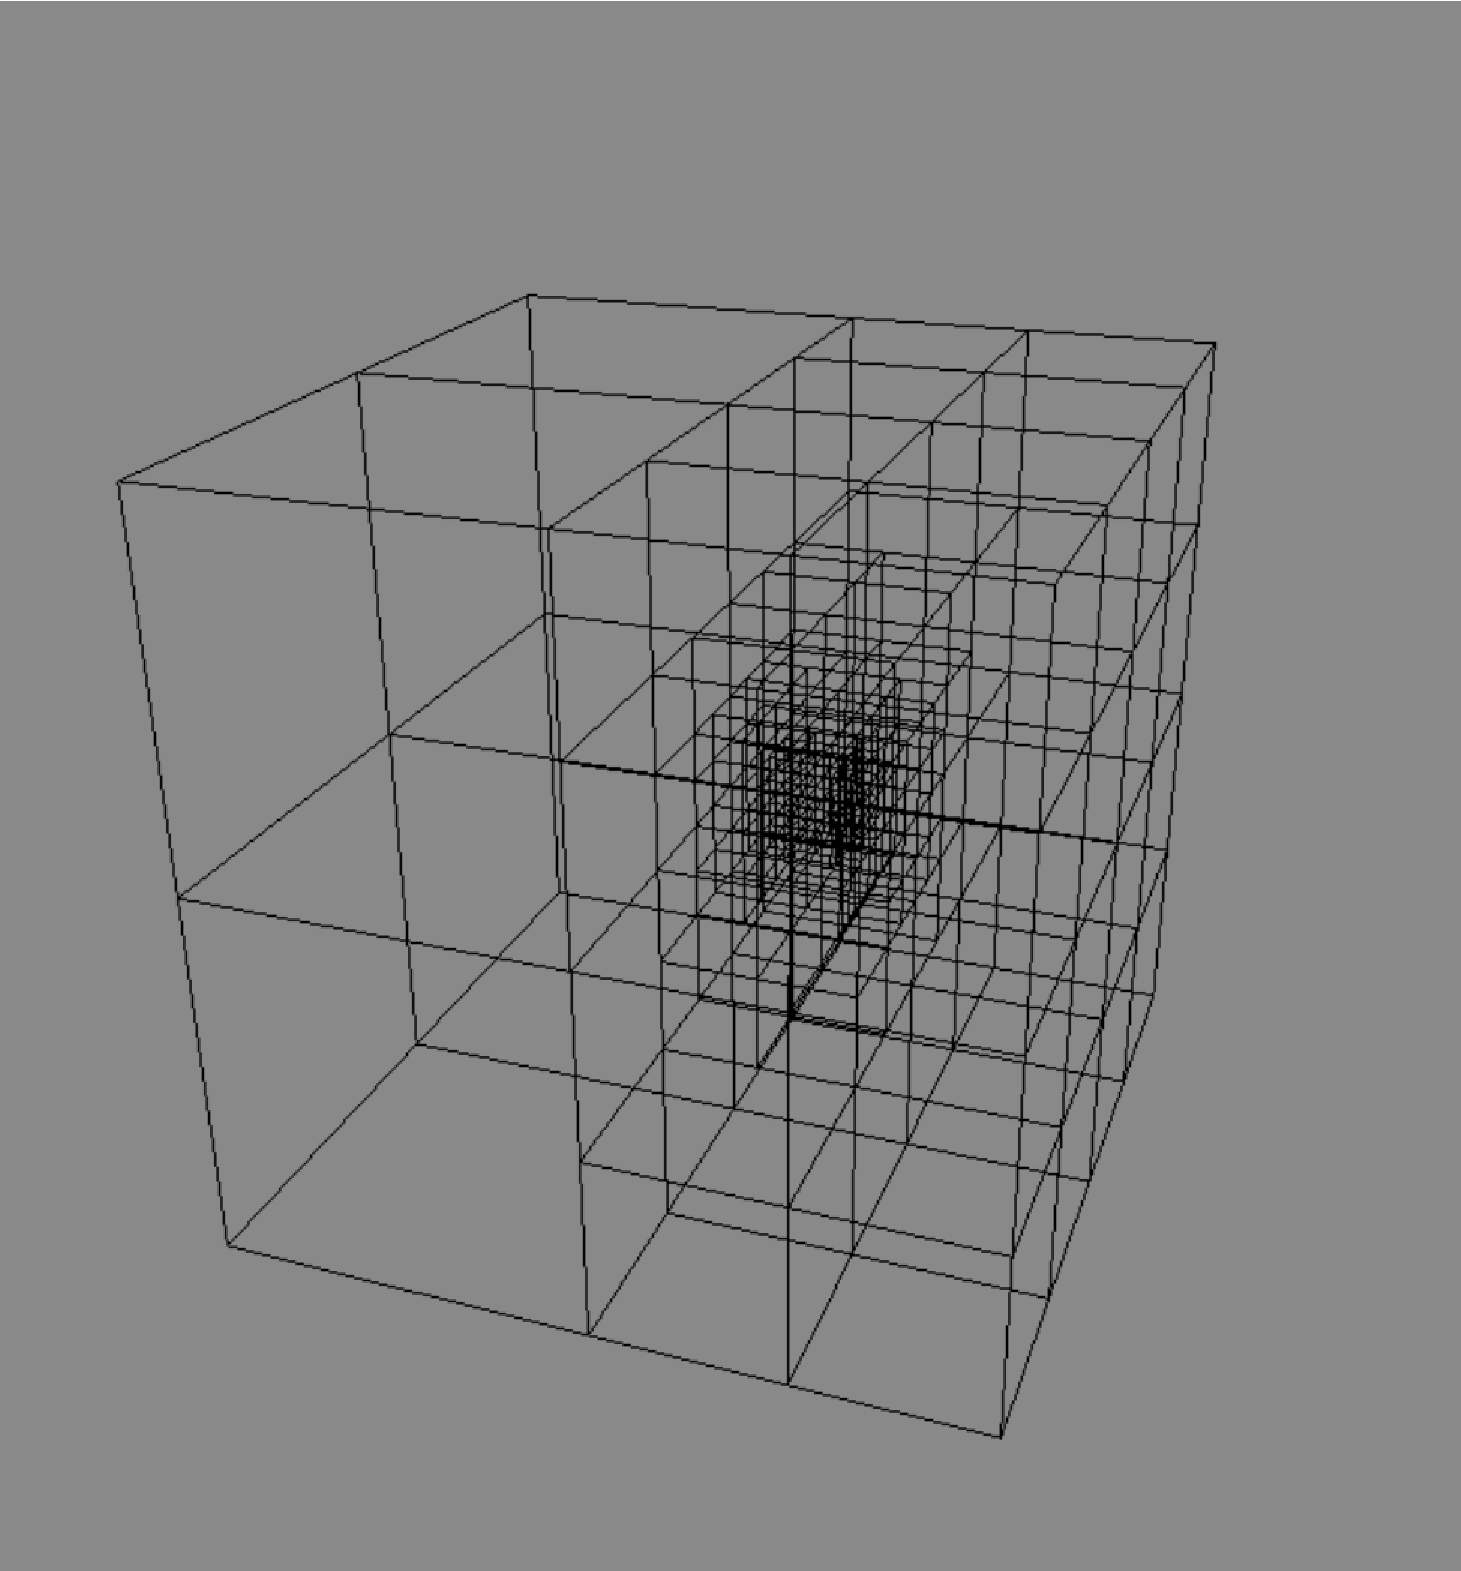
\includegraphics[scale=0.1788]{figures/adapgrid.pdf}
\end{frame}

%\begin{frame}
%\frametitle{Multiwavelets}
%\begin{columns}
%
%\begin{column}[b]{0.55\linewidth}
%\begin{itemize}
%    \item   \textbf{Wavelet functions} are piecewise polynomials
%    \item   \textbf{Wavelet projection} at scale $N$
%	\begin{equation}
%	    \nonumber
%	    df^n(x) = f^{n+1}(x) - f^{n}(x)
%	\end{equation}
%	\ \\
%    \item   Alternative \textbf{multiresolution} representation
%	\begin{equation}
%	    \nonumber
%	    f^N(x) = f^{0}(x) + \sum_{n=0}^{N-1} df^{n}(x)
%	\end{equation}
%    \item   Allows for \textbf{adaptive refinement} by local thresholding
%	\begin{equation}
%	    \nonumber
%	    \|df_l^n\| < \frac{\epsilon}{2^{n/2}}\|f\|
%	\end{equation}
%    \item   Representations with \textbf{guaranteed precision} $\epsilon$
%\end{itemize}
%\ \\
%\ \\
%\end{column}
%
%\begin{column}[b]{0.45\linewidth}
%\centering
%\includegraphics[scale=0.3, clip, viewport=100 400 500 800]
%    {figures/adaptivity.pdf}
%\end{column}
%
%\end{columns}
%\ \\
%\centering
%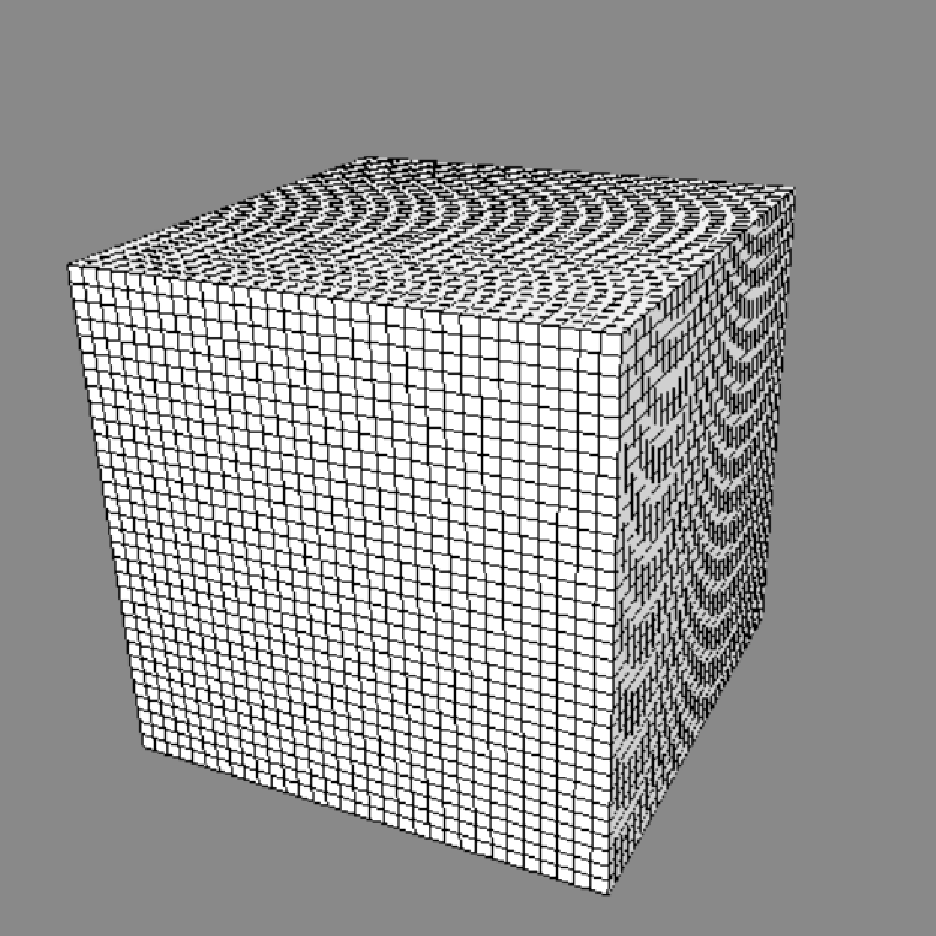
\includegraphics[scale=0.2]{figures/unifgrid.pdf}
%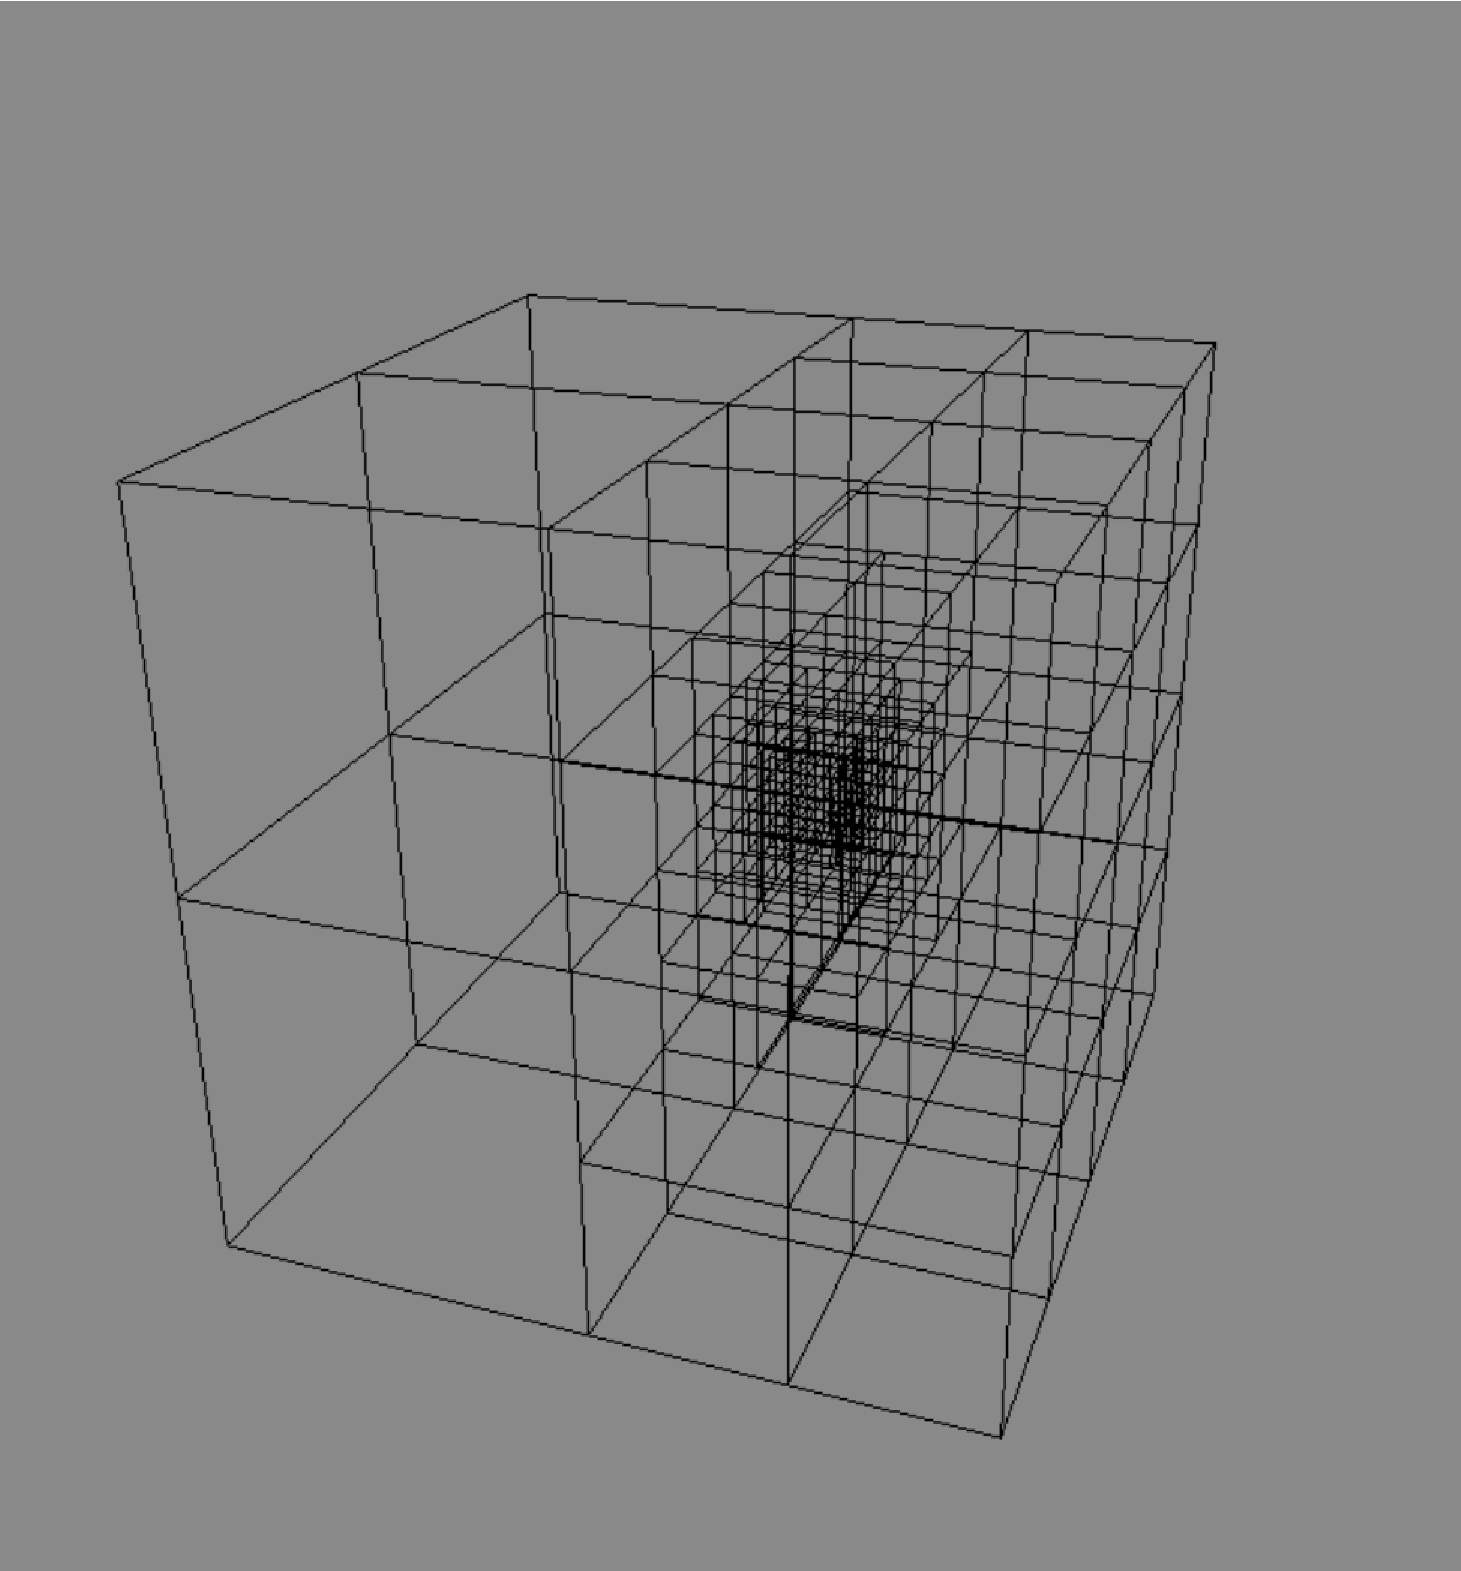
\includegraphics[scale=0.1192]{figures/adapgrid.pdf}
%\end{frame}


%\begin{frame}
%    \frametitle{Decreasing order polynomial basis}
%    \begin{columns}
%    \begin{column}[b]{0.7\linewidth}
%	\begin{itemize}
%	    \item   Multi-dimensional functions require many expansion coefficients\\
%		    \ \\
%	    \item   Try to reduce the memory footprint by varying the polynomial order\\
%		    \ \\
%	    \item   Specifically decreasing the order $k$ with increasing scale $n$
%	\end{itemize}
%	\ \\
%	\ \\
%	\ \\
%    \end{column}
%    \begin{column}[b]{0.3\linewidth}
%    \centering
%    \begin{figure}
%	\setlength{\unitlength}{.5mm}
%	\begin{picture}(93,46)
%	    \put( 0,10){\vector(1,0){60}} n- axis
%	    \put(61,10){$n$}
%	    \put(10,4){\vector(0,1){37}} k-axis
%	    \put(10,43){$k$}
%	    \put(40,38){$k(n)$}
%	    \put(-5,30){$k_{\max}$}
%	    \put(-5,15){$k_{\min}$}
%	    \put(25,5){$n_0$}
%	    \put(40,5){$n_1$}
%	    \put(10,30){\line(1,0){15}}
%	    \put(25,30){\line(1,-1){15}}
%	    \put(40,15){\line(1,0){15}}
%	    \multiput(40,10)(0,0.1){5}{\line(0,1){2}} 
%	    \multiput(25,10)(0,4){5}{\line(0,1){2}}
%	    \multiput(10,15)(6,0){5}{\line(1,0){2}}
%	\end{picture}
%    \end{figure}
%    \end{column}
%    \end{columns}
%    \ \\
%    \centering
%    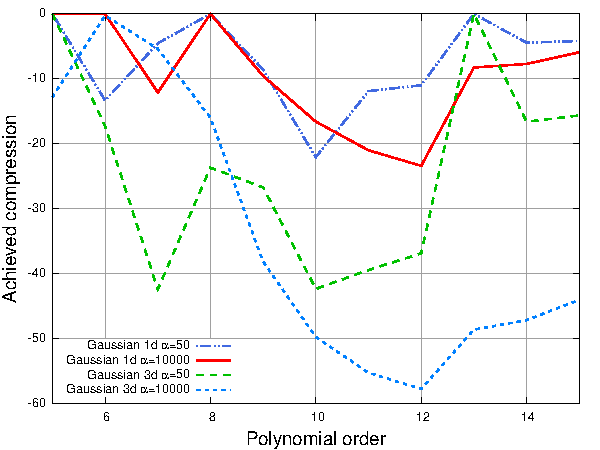
\includegraphics[scale=0.6]{figures/decrease.pdf}
%\end{frame}


%\begin{frame}
    \centering
    \Large{Part II:}\\
    \ \\
    \ \\
    \centering
    \Large{Linear scaling Coulomb interaction in the multiwavelet basis,\\
	a parallel implementation}
\end{frame}

\begin{frame}
    \frametitle{Operator representation}
    \begin{columns}
    \begin{column}[b]{0.5\linewidth}
    \begin{itemize}
	\item	The multiwavelet basis is well suited for\\ \textbf{integral convolution operators}
	    \begin{equation}
		\nonumber
		g(\boldsymbol{r}) = \left[T f\right](\boldsymbol{r}) = 
		    \int K(\boldsymbol{r} - \boldsymbol{r'})f(\boldsymbol{r'}) d\boldsymbol{r'}
	    \end{equation}
	    \ \\
	    \ \\
	\item \textbf{Scaling projection} of operator at scale $n$
	    \begin{equation}
		\nonumber
		T \approx T^n
	    \end{equation}
	\item \textbf{Wavelet projections} obtained by the difference
	    \begin{equation}
		\nonumber
		T^{n+1} - T^n = A^n + B^n + C^n
	    \end{equation}
	\item \textbf{Multiresolution operator} obtained by recursion
	    \begin{equation}
		\nonumber
		T^N = T^0 + \sum_{n=0}^{N-1} \left[A^n + B^n + C^n\right]
	    \end{equation}
	\item Scaling operator $T$ is \textbf{dense}
	\item Wavelet operators $A$, $B$ and $C$ are \textbf{sparse} 
    \end{itemize}
    \end{column}
    \begin{column}[b]{0.5\linewidth}
    \begin{center}
    \only<2>{\ \ \ 
\includegraphics[scale=0.6, clip, viewport = 240 280 450 480]{figures/matrix/matrix_1.pdf}}
    \only<3>{\ \ 
\includegraphics[scale=0.6, clip, viewport = 240 280 450 480]{figures/matrix/matrix_2.pdf}}
    \only<4>{\ 
\includegraphics[scale=0.6, clip, viewport = 240 280 450 480]{figures/matrix/matrix_3.pdf}}
    \only<5>{
\includegraphics[scale=0.6, clip, viewport = 240 280 450 480]{figures/matrix/matrix_4.pdf}}
    \only<6>{
\includegraphics[scale=0.6, clip, viewport = 240 280 450 480]{figures/matrix/matrix_5.pdf}}
    \only<7,8>{
\includegraphics[scale=0.6, clip, viewport = 240 280 450 480]{figures/matrix/matrix_6.pdf}}
    \ \\
    \ \\
    \ \\
    \end{center}
    \end{column}
    \end{columns}
    \ \\
    \ \\
    \ \\
    \ \\
    \pause
    \pause
    \pause
    \pause
    \pause
    \pause
    \pause
    \begin{columns}
    \begin{column}{.48\textwidth}
    \centering
    \textbf{Poisson kernel}
    \begin{equation}
	\nonumber
	P(\boldsymbol{r}-\boldsymbol{r}') = 
	    \frac{1}{4\pi}\ \frac{1}{|\boldsymbol{r}-\boldsymbol{r}'|}
    \end{equation}
    \end{column}
    \begin{column}{.48\textwidth}
    \centering
    \textbf{Helmholtz kernel}
    \begin{equation}
	\nonumber
	H^{\mu}(\boldsymbol{r}-\boldsymbol{r}') = \frac{1}{4\pi}\ 
	    \frac{e^{-\mu |\boldsymbol{r}-\boldsymbol{r}'|}}{|\boldsymbol{r}-\boldsymbol{r}'|}
    \end{equation}
    \end{column}
    \end{columns}    
\end{frame}

\begin{frame}
    \frametitle{Coulomb interaction}
    \begin{itemize}
	\item	Electrostatic potential from a \textbf{point charge} follows from Coulomb's law
		\begin{equation}
		    \nonumber
		    V(\boldsymbol{r}) = \frac{q}{4\pi\epsilon_0}
		    \frac{1}{|\boldsymbol{r}-\boldsymbol{r}'|}
		\end{equation}
		\ \\
		\ \\
		\ \\
	\item	Electrostatic potential from a \textbf{charge density} is given by the Poisson equation
		\begin{equation}
		    \nonumber
		    \nabla^2 V(\boldsymbol{r}) = -\rho(\boldsymbol{r})
		\end{equation}
		\ \\
		\ \\
		\ \\
	\item	Can be solved directly in integral form using the Poisson kernel
		\begin{equation}
		    \nonumber
		    V(\boldsymbol{r}) = 
		    \int P(\boldsymbol{r}-\boldsymbol{r'})\rho(\boldsymbol{r'}) d\boldsymbol{r'} =
		    \int\frac{\rho(\boldsymbol{r'})}{4\pi|\boldsymbol{r} - \boldsymbol{r'}|} d\boldsymbol{r'} 
		\end{equation}
		\ \\
		\ \\
		\ \\
    \end{itemize}
    \ \\
    \ \\
    \ \\
    \begin{columns}
    \begin{column}{.30\textwidth}
        \ \\
    \end{column}
    \begin{column}{.40\textwidth}
        \ \ \ \ \textbf{Numerical problems}
        \begin{itemize}
	    \item Not Cartesian separable
	    \item Singularity at short-range
	    \item Slow decay at long-range
	\end{itemize}
    \end{column}
    \begin{column}{.30\textwidth}
	\ \\
    \end{column}
    \end{columns}
\end{frame}

\begin{frame}
    \frametitle{Separation of variables using Gaussians}
    \begin{columns}
    \begin{column}{.50\textwidth}
    \begin{itemize}
	\item The Poisson kernel can be approximated as
	    \begin{equation}
		\nonumber
		\frac{1}{\boldsymbol{r}} \approx \sum_{i=1}^M a_i e^{-\alpha_i \boldsymbol{r}^2} 
	    \end{equation}
	\item Any accuracy can in principle be obtained
	\item Full operator is decomposed into $M$ terms
	\item Each operator term is applied separately
    \end{itemize}
    \ \\
    \ \\
    \ \\
    \ \\
    \ \\
    \pause
    \pause
    \pause
    \pause
    \pause
    \pause
    \pause
    \ \ \ \ \textbf{Solves problems}
    \begin{itemize}
	\item	Separates coordinates
	\item	Removes singularity
	\item	Separates length scales
    \end{itemize}
    \end{column}
    \begin{column}{.50\textwidth}
	\only<1,2,3,4,5>{\ \\}
	\only<1>{\ \ \ \ \ \ \ 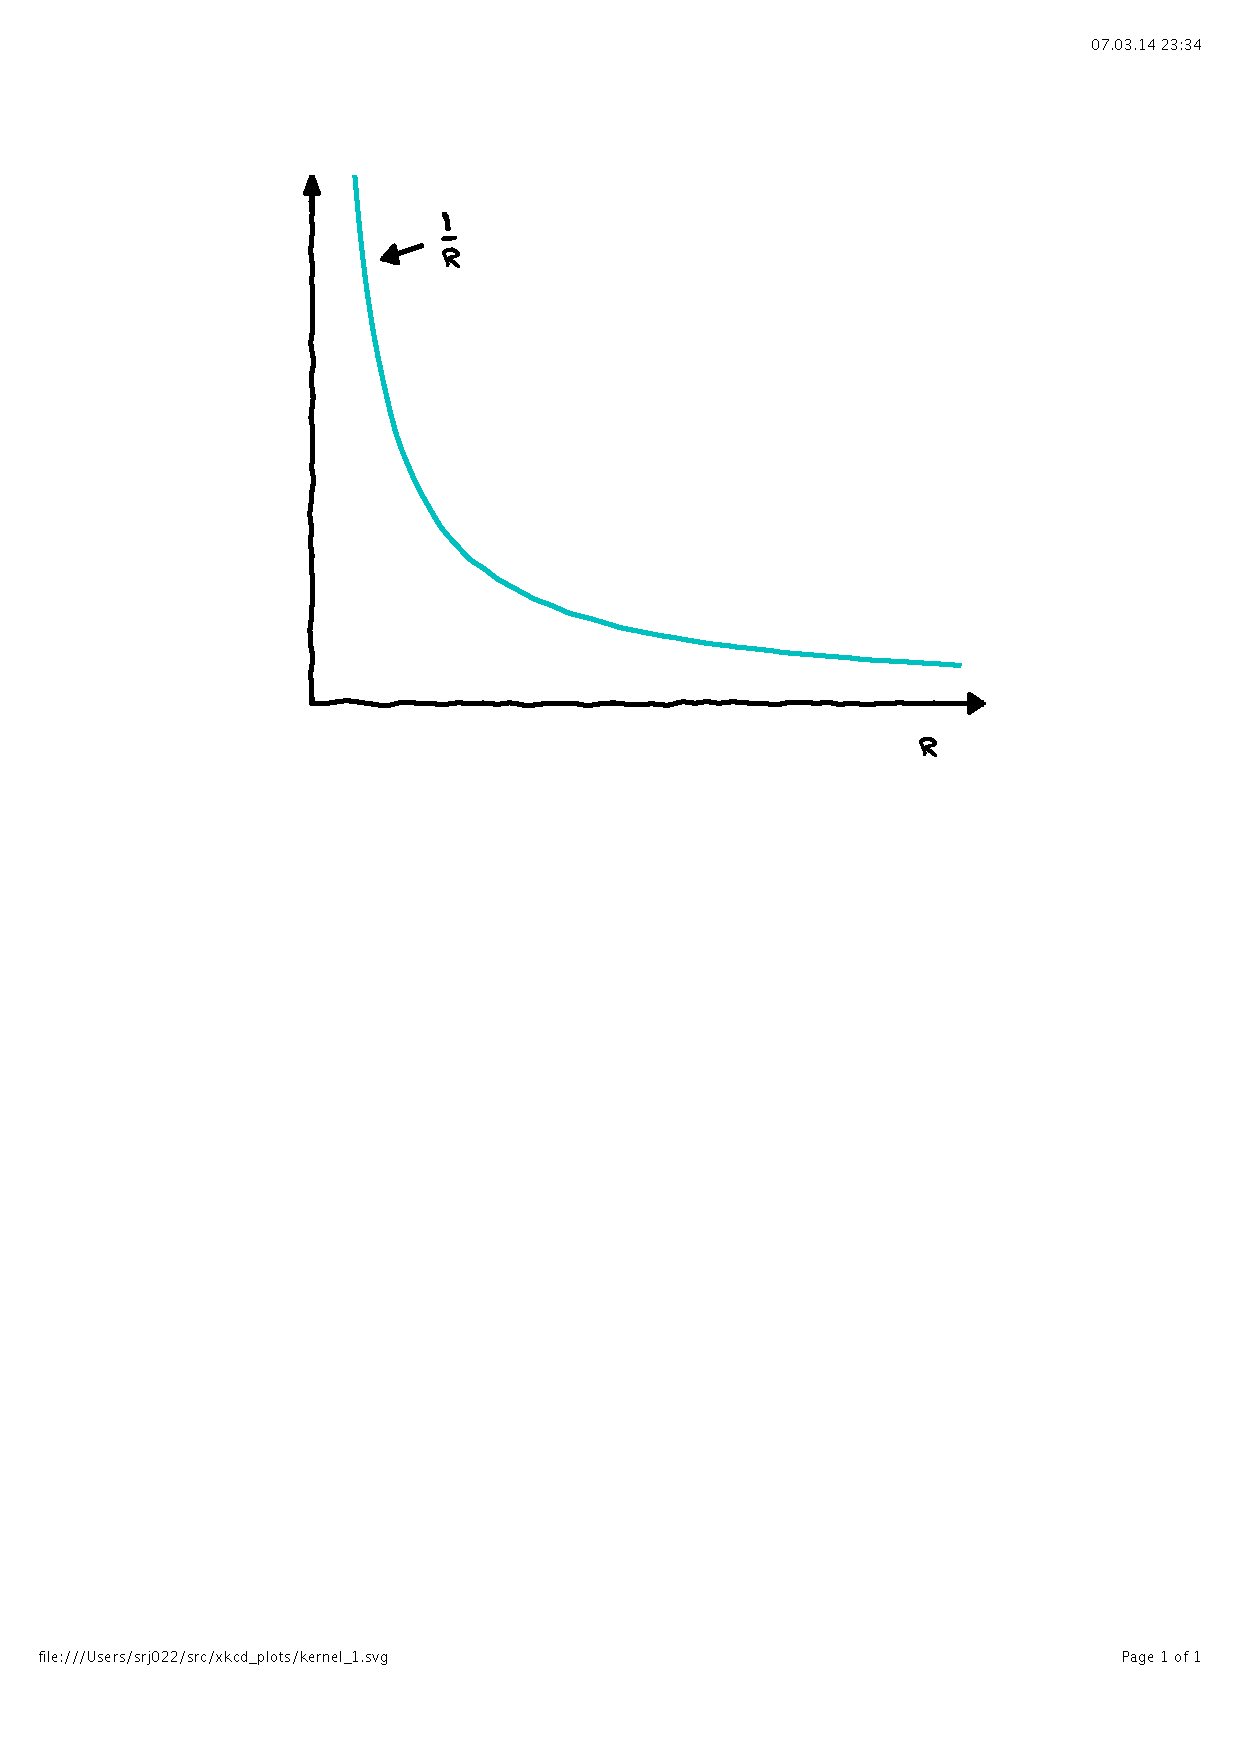
\includegraphics[scale=0.4, clip, viewport = 110 450 490 800]{figures/kernel_1.pdf}}
	\only<2>{\ \ \ \ \ \ 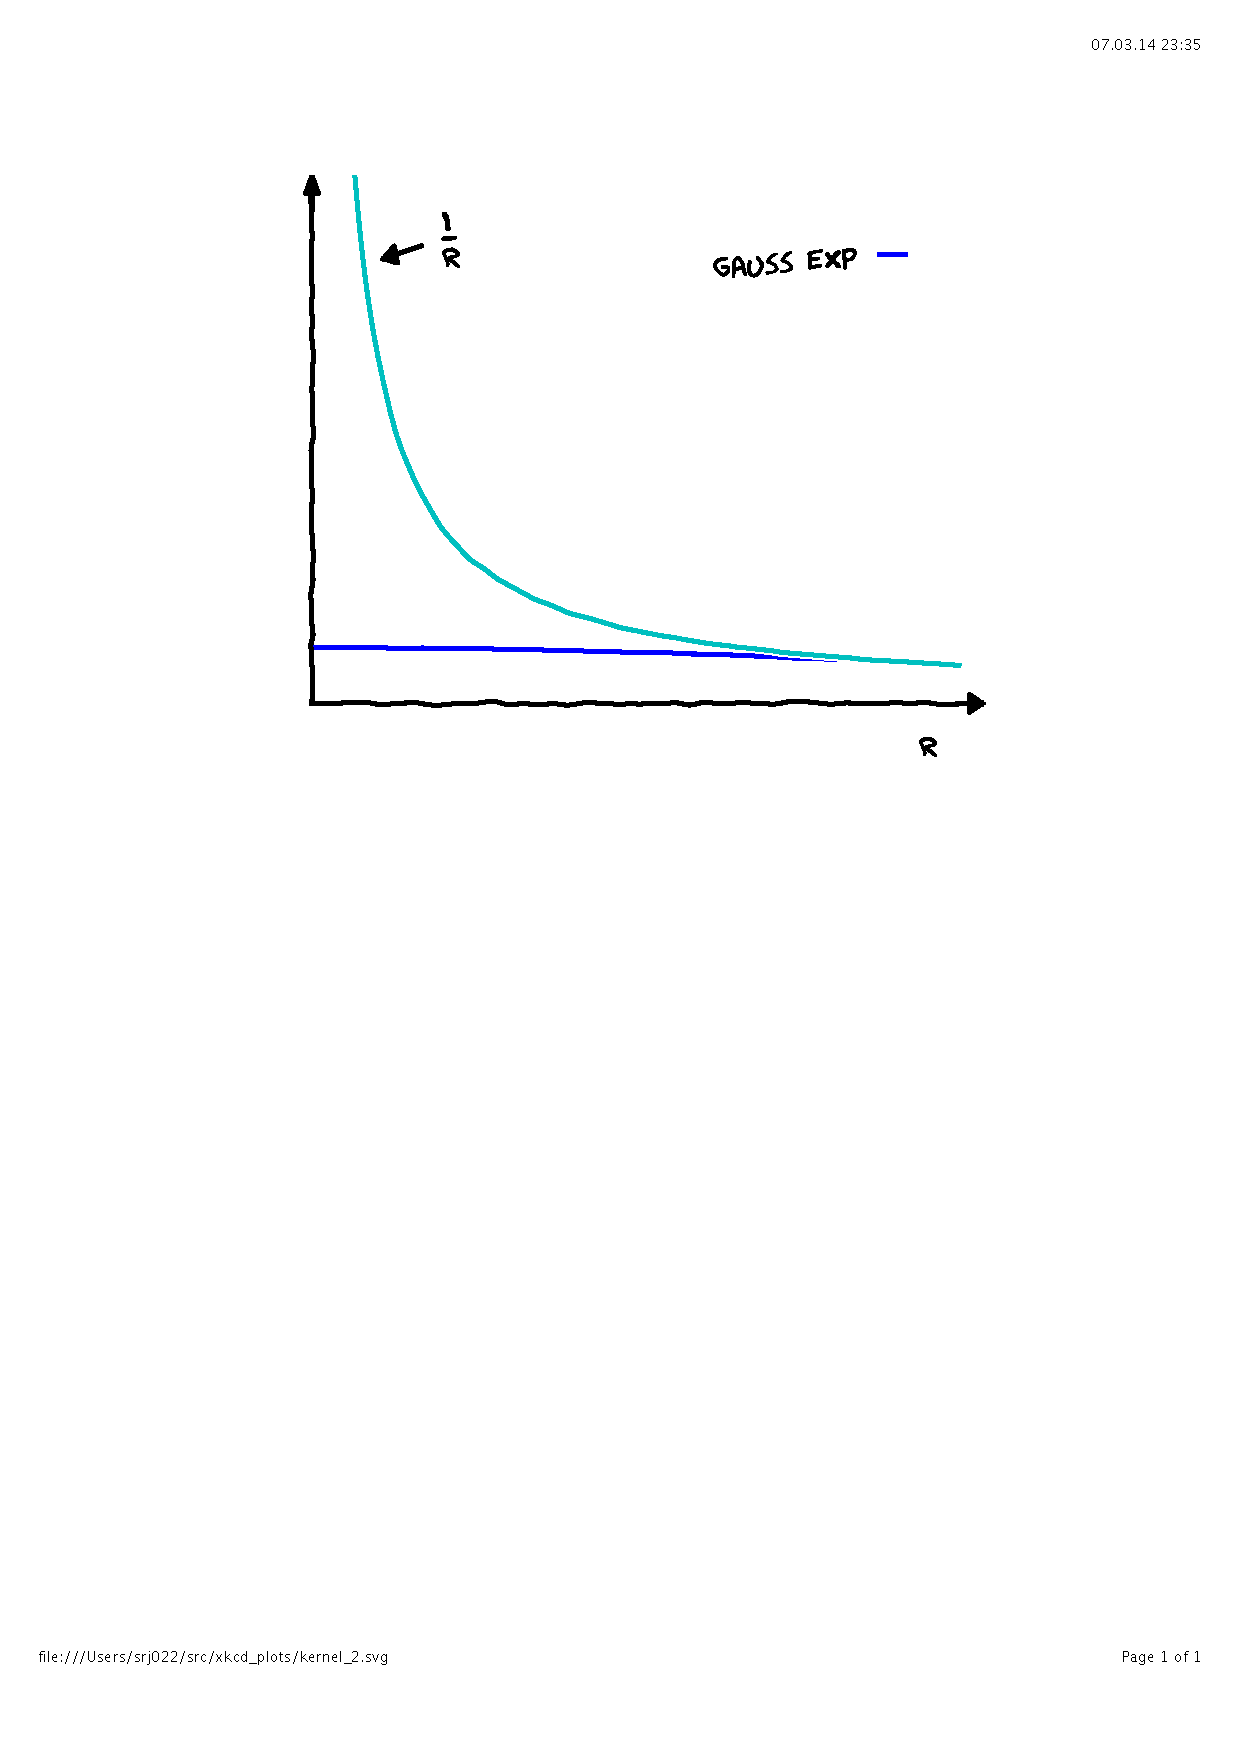
\includegraphics[scale=0.4, clip, viewport = 110 450 490 800]{figures/kernel_2.pdf}}
	\only<3>{\ \ \ \ \ 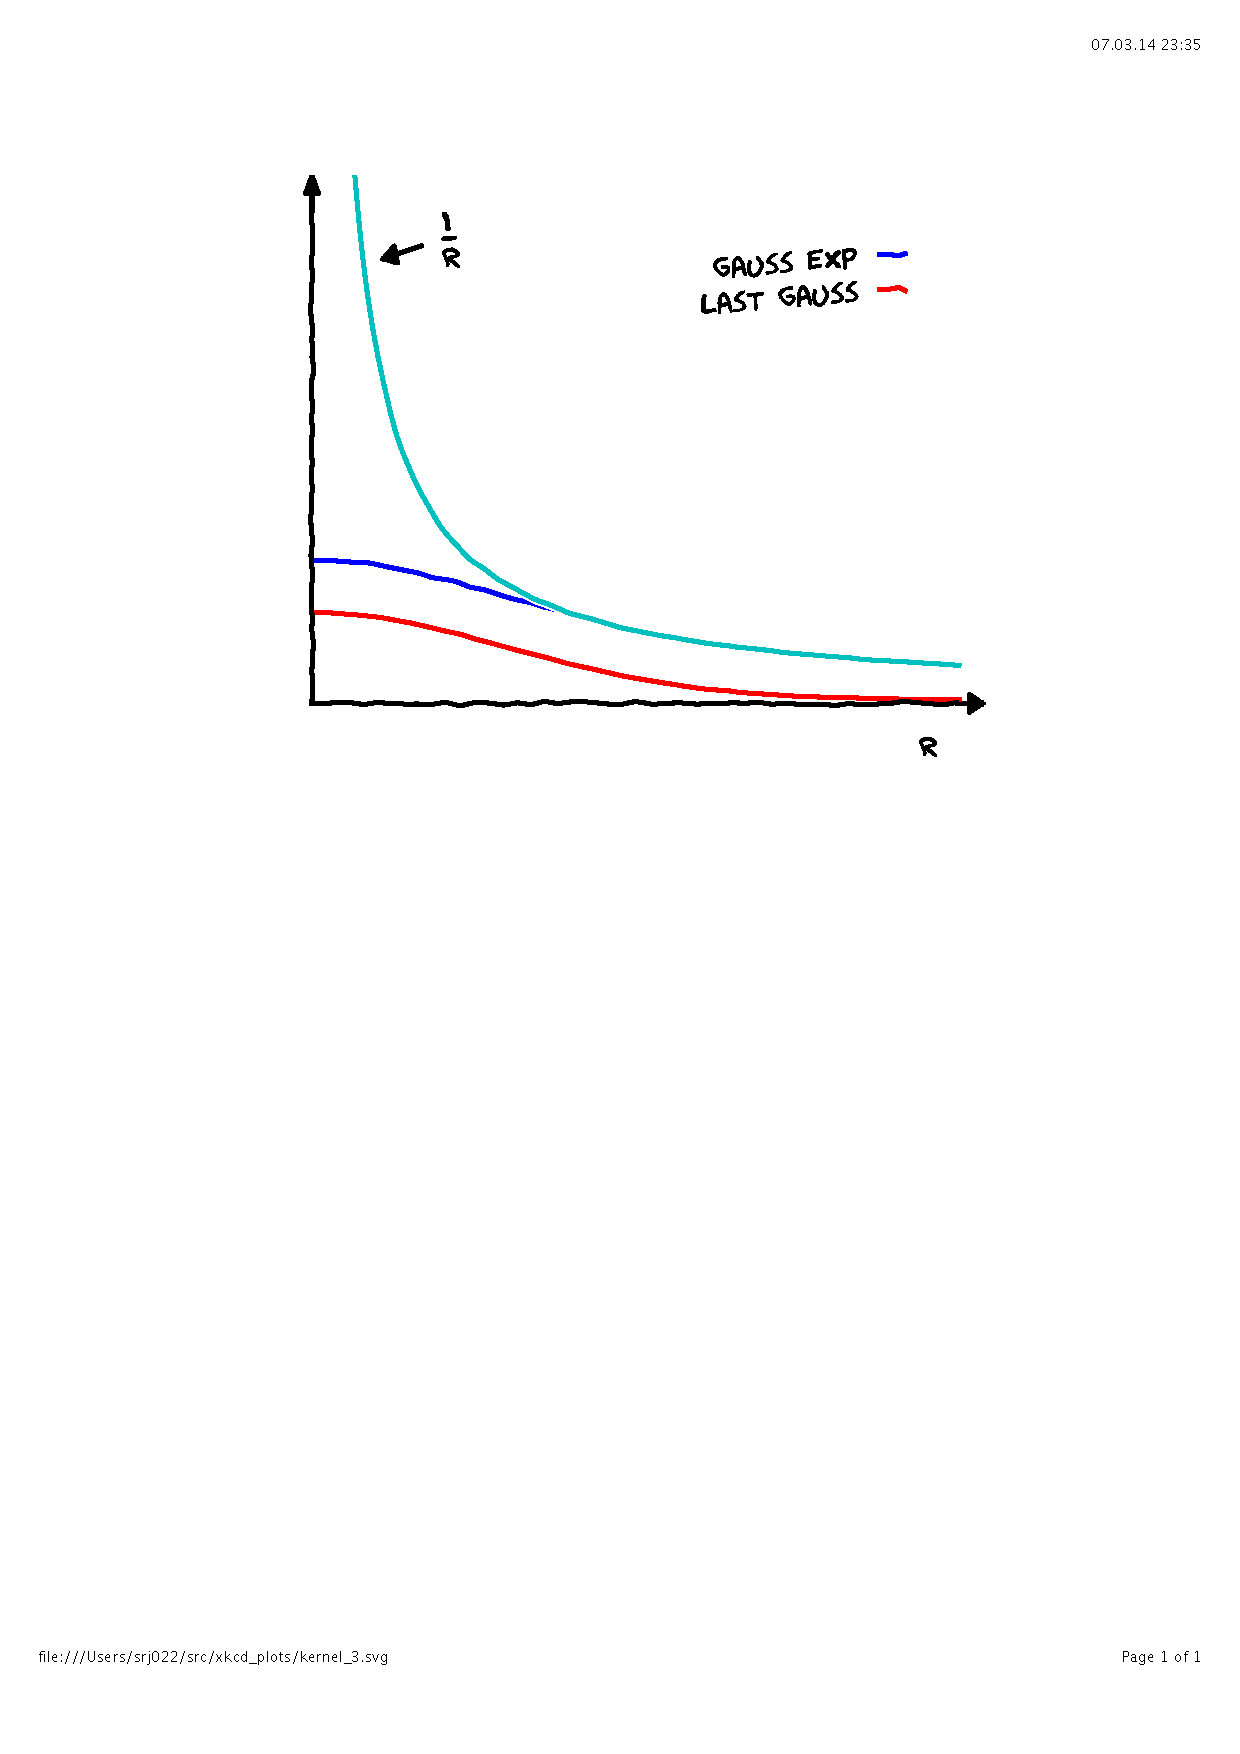
\includegraphics[scale=0.4, clip, viewport = 110 450 490 800]{figures/kernel_3.pdf}}
	\only<4>{\ \ \ \ 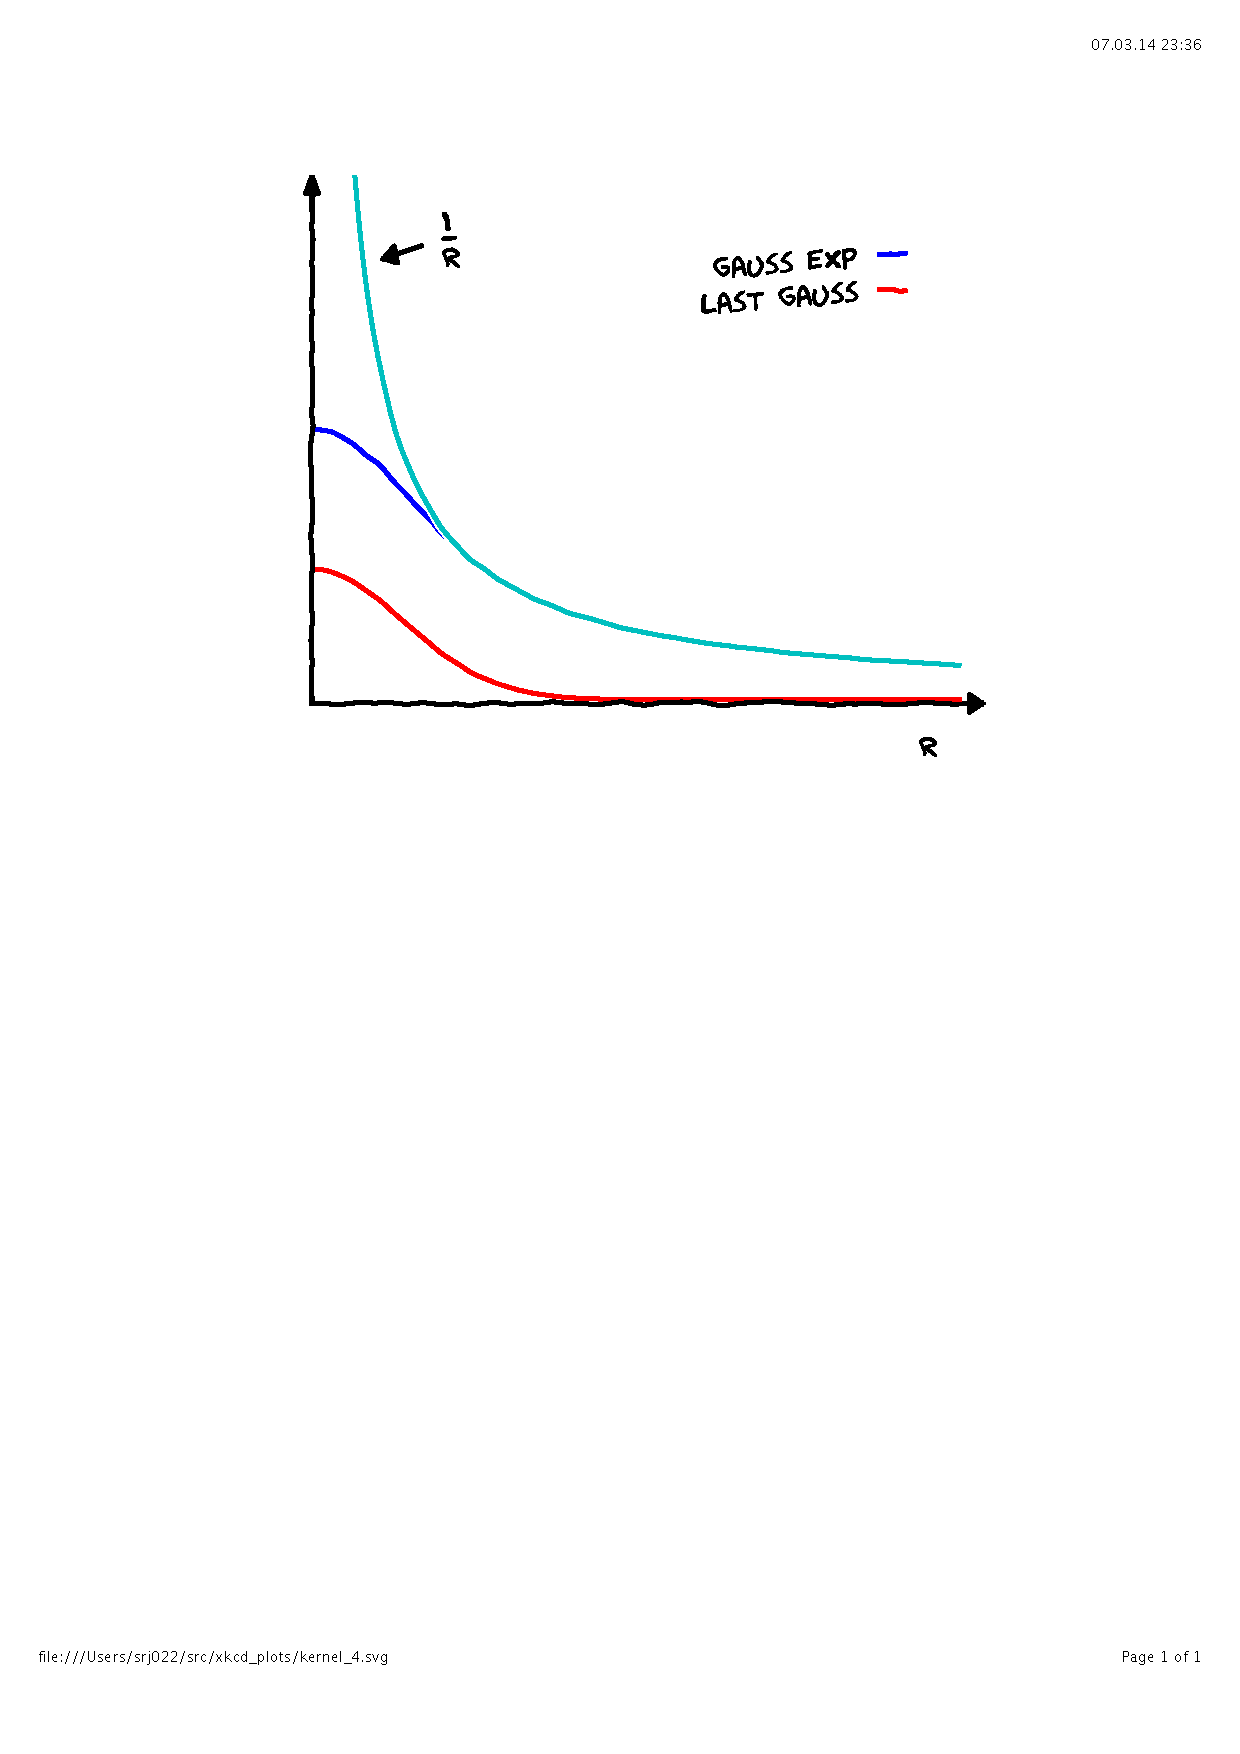
\includegraphics[scale=0.4, clip, viewport = 110 450 490 800]{figures/kernel_4.pdf}}
	\only<5>{\ \ \ 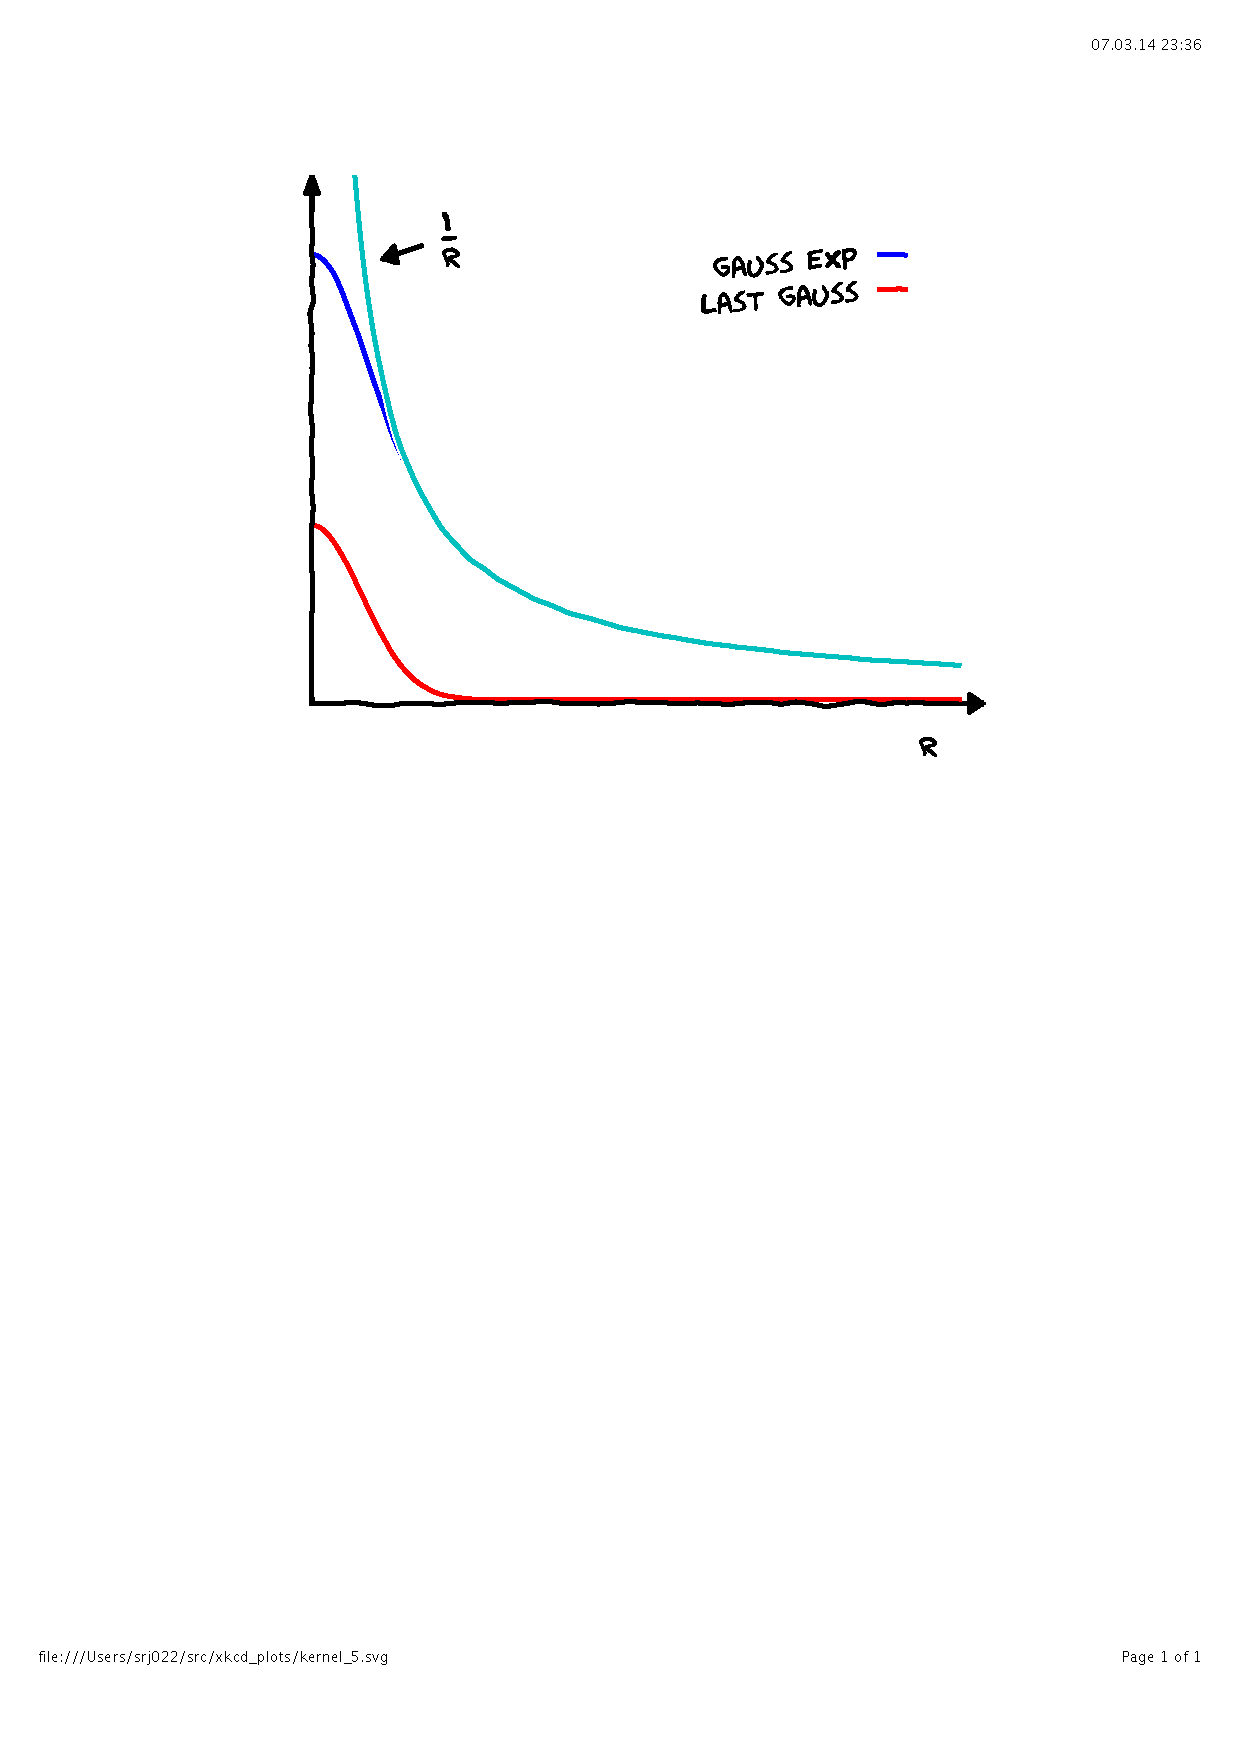
\includegraphics[scale=0.4, clip, viewport = 110 450 490 800]{figures/kernel_5.pdf}}
	\only<6>{\ \ 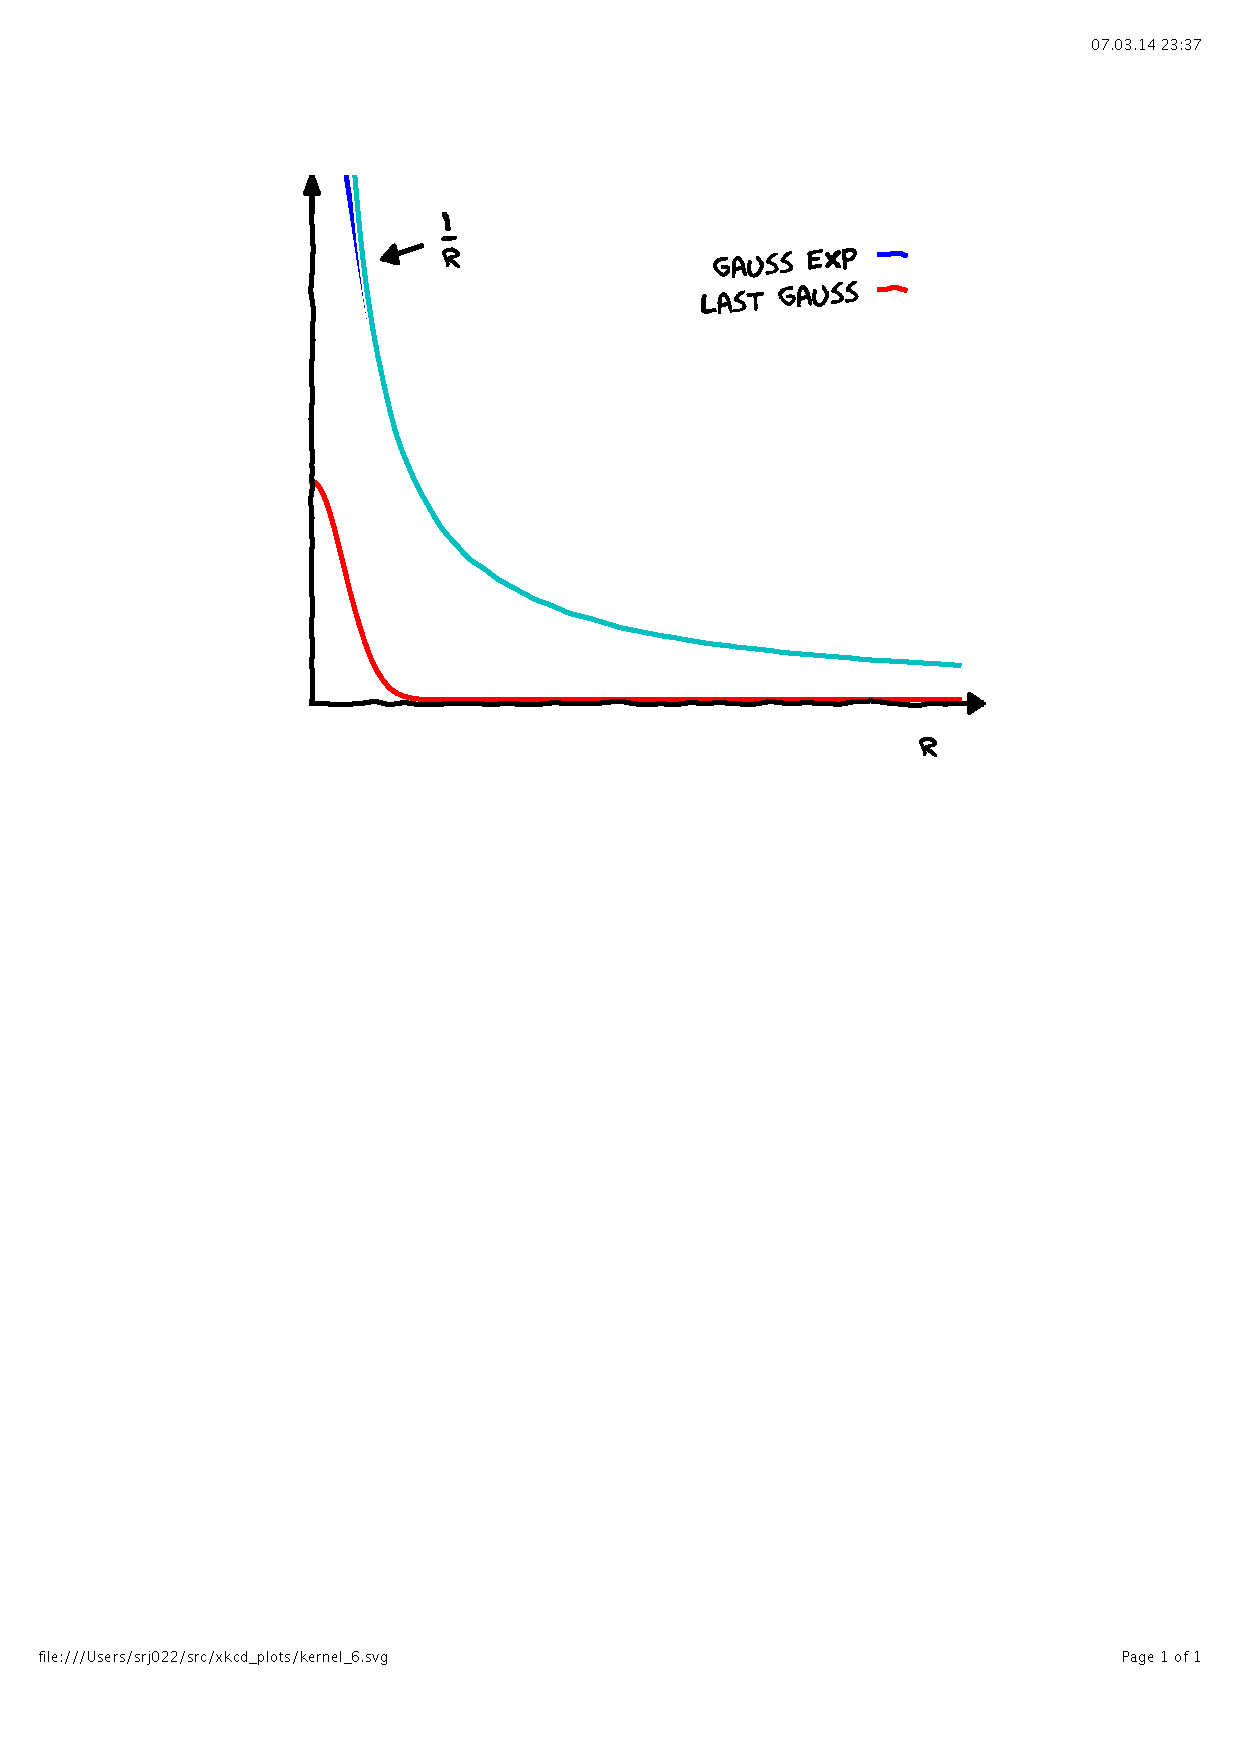
\includegraphics[scale=0.4, clip, viewport = 110 450 490 800]{figures/kernel_6.pdf}}
	\only<7,8>{\ 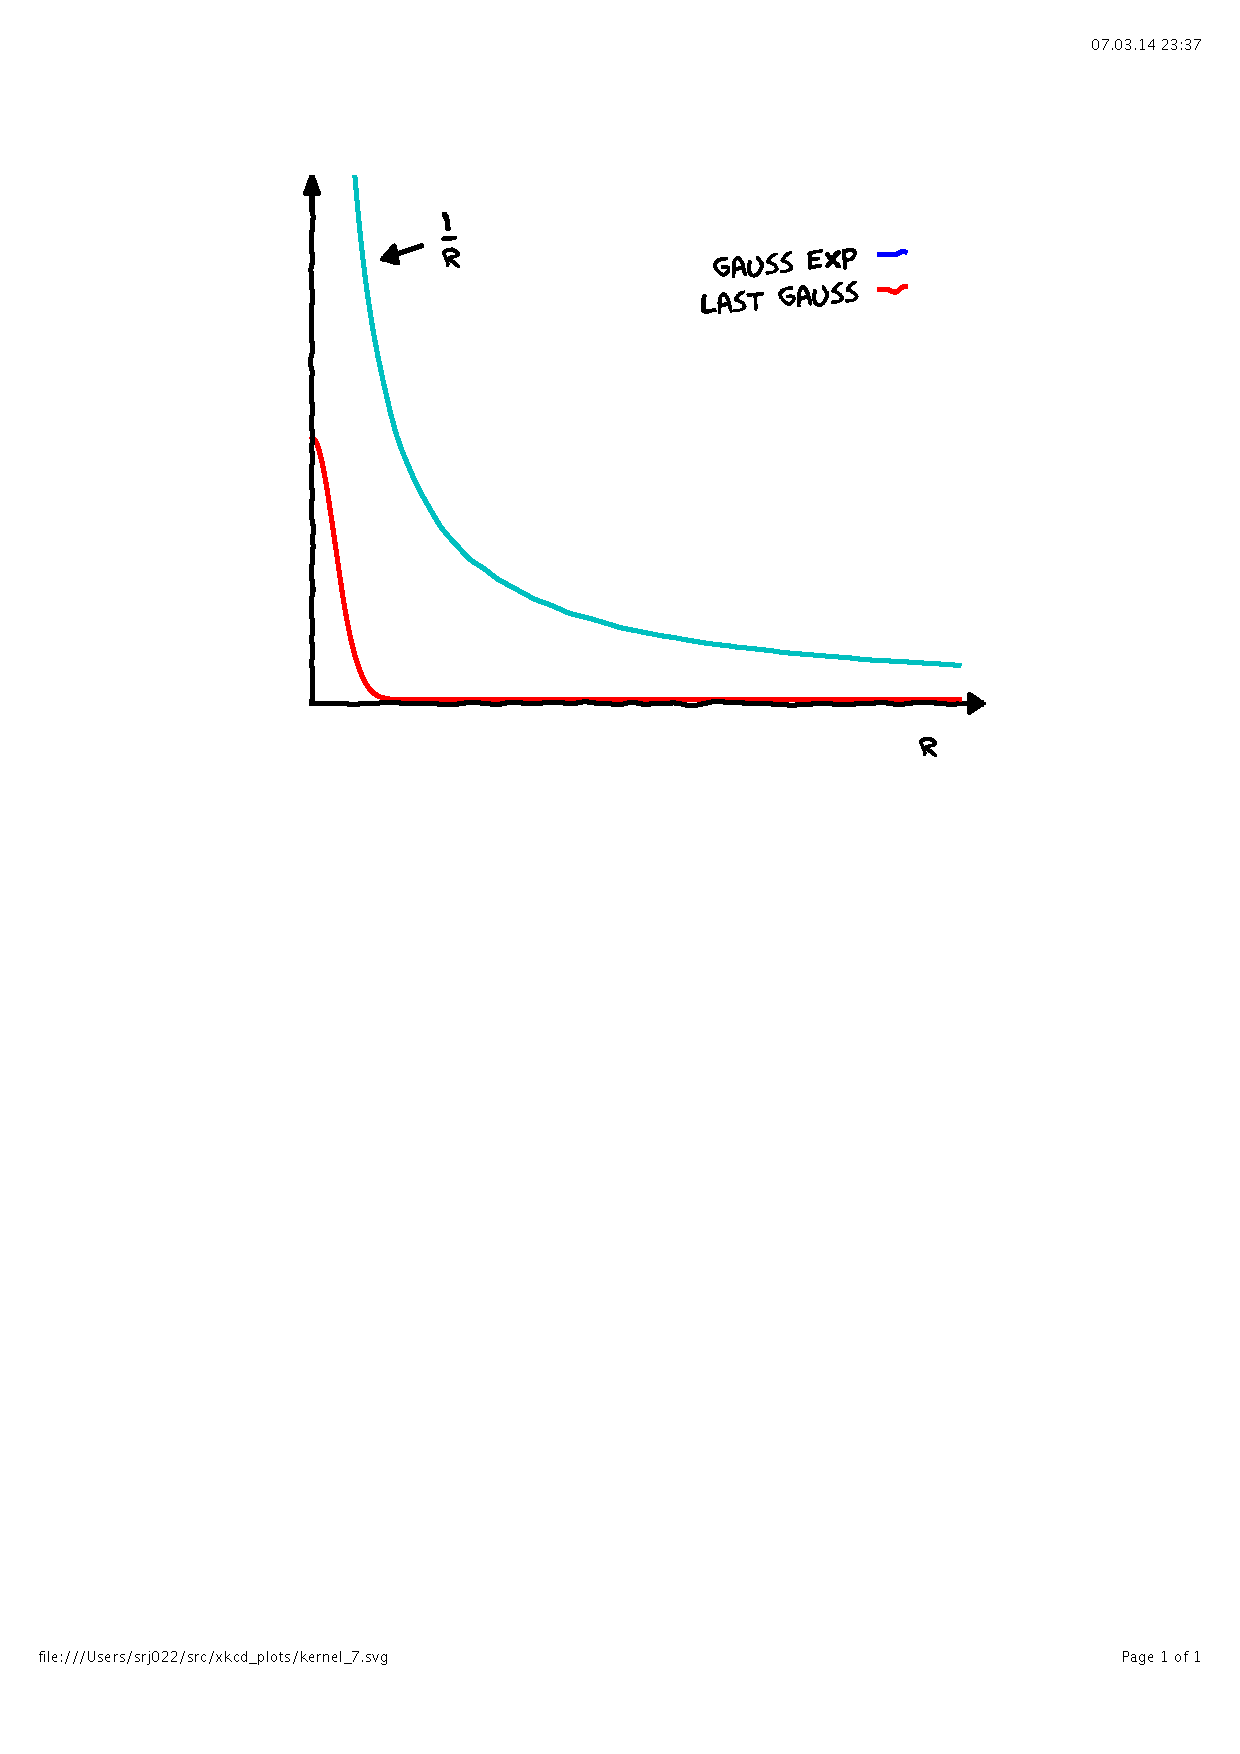
\includegraphics[scale=0.4, clip, viewport = 110 450 490 800]{figures/kernel_7.pdf}}
    \end{column}
    \end{columns}    
    \ \\
    \ \\
    \ \\
    \ \\
    \ \\
    \ \\
    \centering
    \only<1,2,3,4,5,6,7>{\ \\ \ \\}
    \only<8>{\normalsize{Combined with the sparse wavelet representation of operators we get\\
	\textbf{linear scaling algorithms}}}
\end{frame}

%\begin{frame}
    %\frametitle{Linear scaling Coulomb interaction}
    %\begin{columns}
    %\begin{column}{.10\textwidth}
    %\ \\
    %\end{column}
    %\begin{column}{.40\textwidth}
	%\centering
	%\ \\
	%\ \\
	%\ \\
	%\ \\
	%Alkane chains
	%\begin{equation}
	    %\nonumber
	    %C_{n}H_{2n+2}, \qquad n=2,\dots,70
	%\end{equation}
	%\ \\
	%\ \\
	%\ \\
	%Fitted curve
	%\begin{equation}
	    %\nonumber
	    %t(n) = 12.5 + 2.34n^{0.754} 
	%\end{equation}
    %\end{column}
    %\begin{column}{.50\textwidth}
	%\centering
	%\begin{figure}
	    %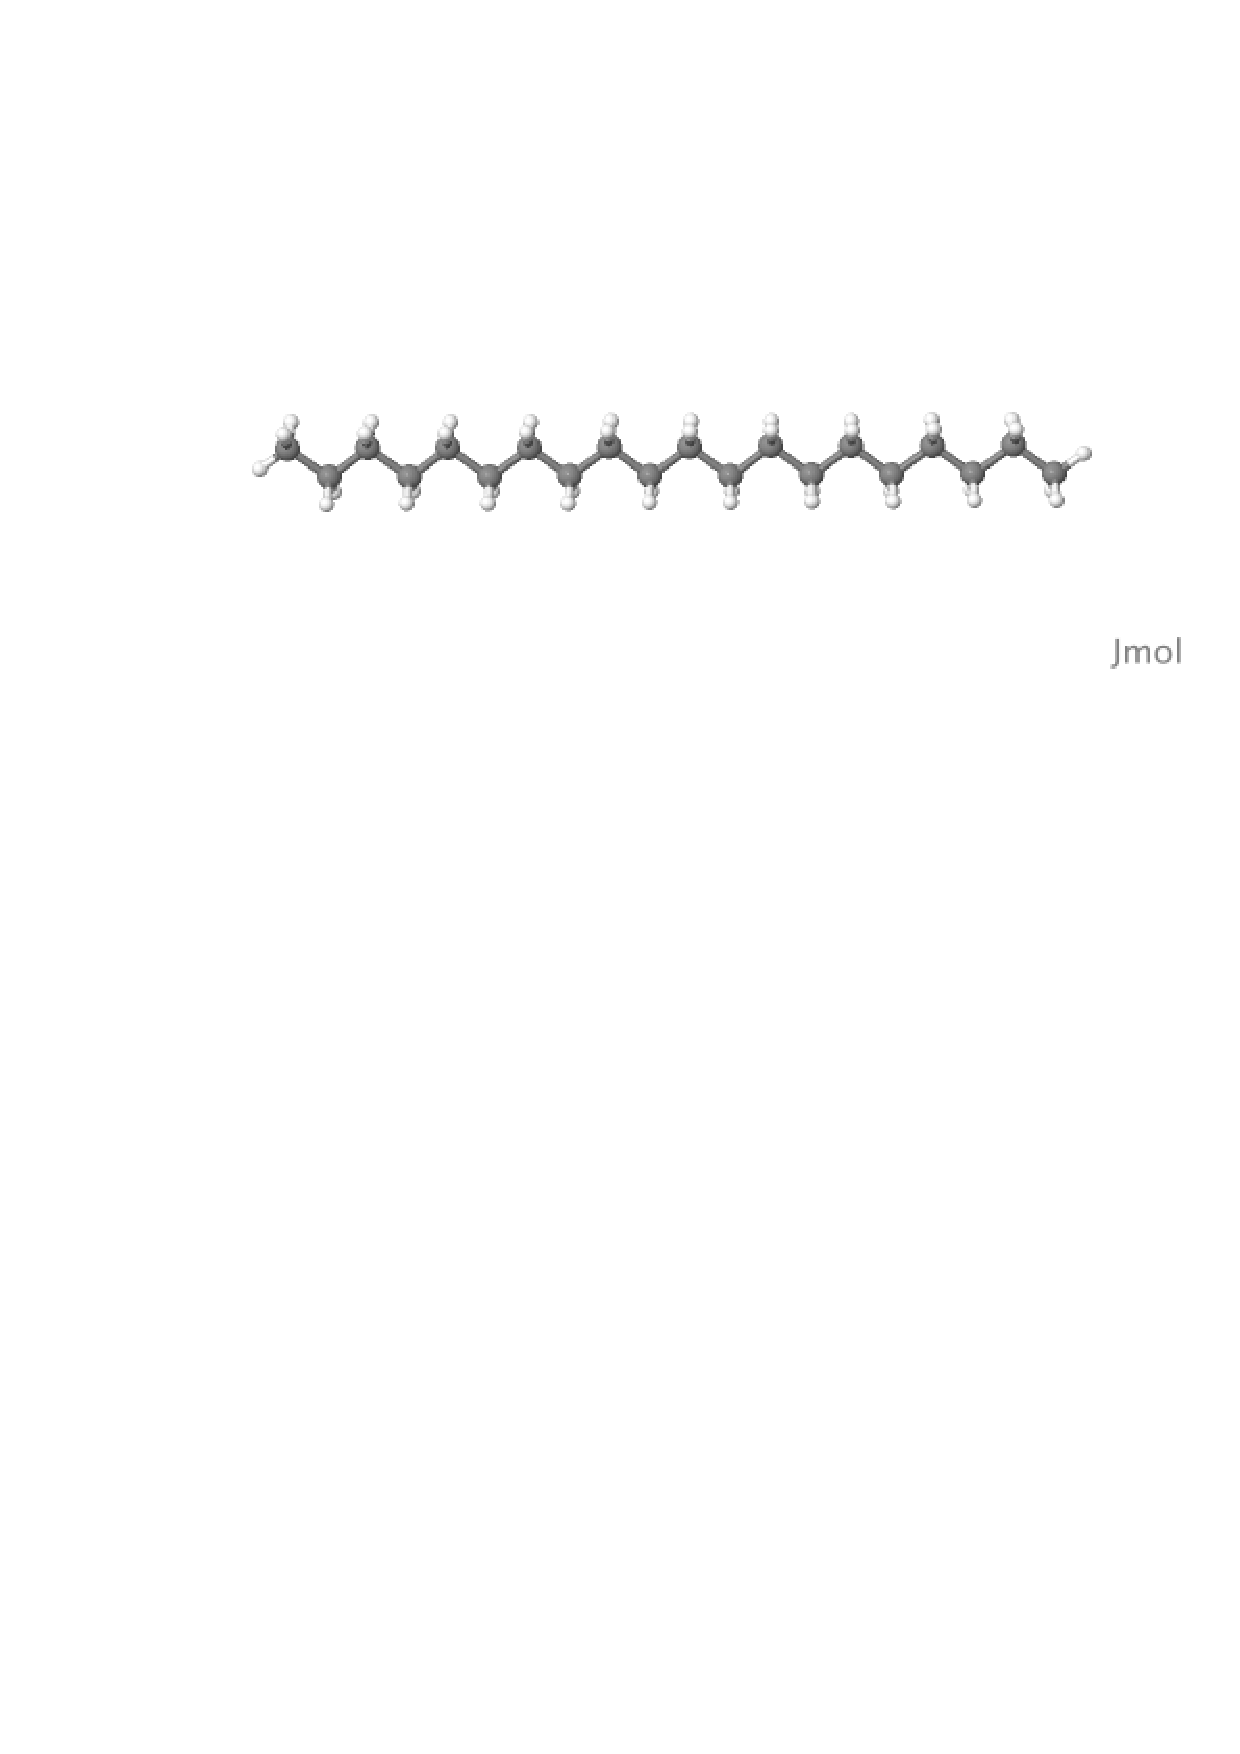
\includegraphics[scale=0.3, clip, viewport = 80 560 600 720]{figures/alkane.pdf}
	%\end{figure}
	%Fitted curve
	%\begin{equation}
	    %\nonumber
	    %t(n) = -6.0 + 1.33n^{0.991}
	%\end{equation}
	%\ \\
	%\ \\
    %\end{column}
    %\end{columns}    
    %\ \\
    %\begin{center}
	%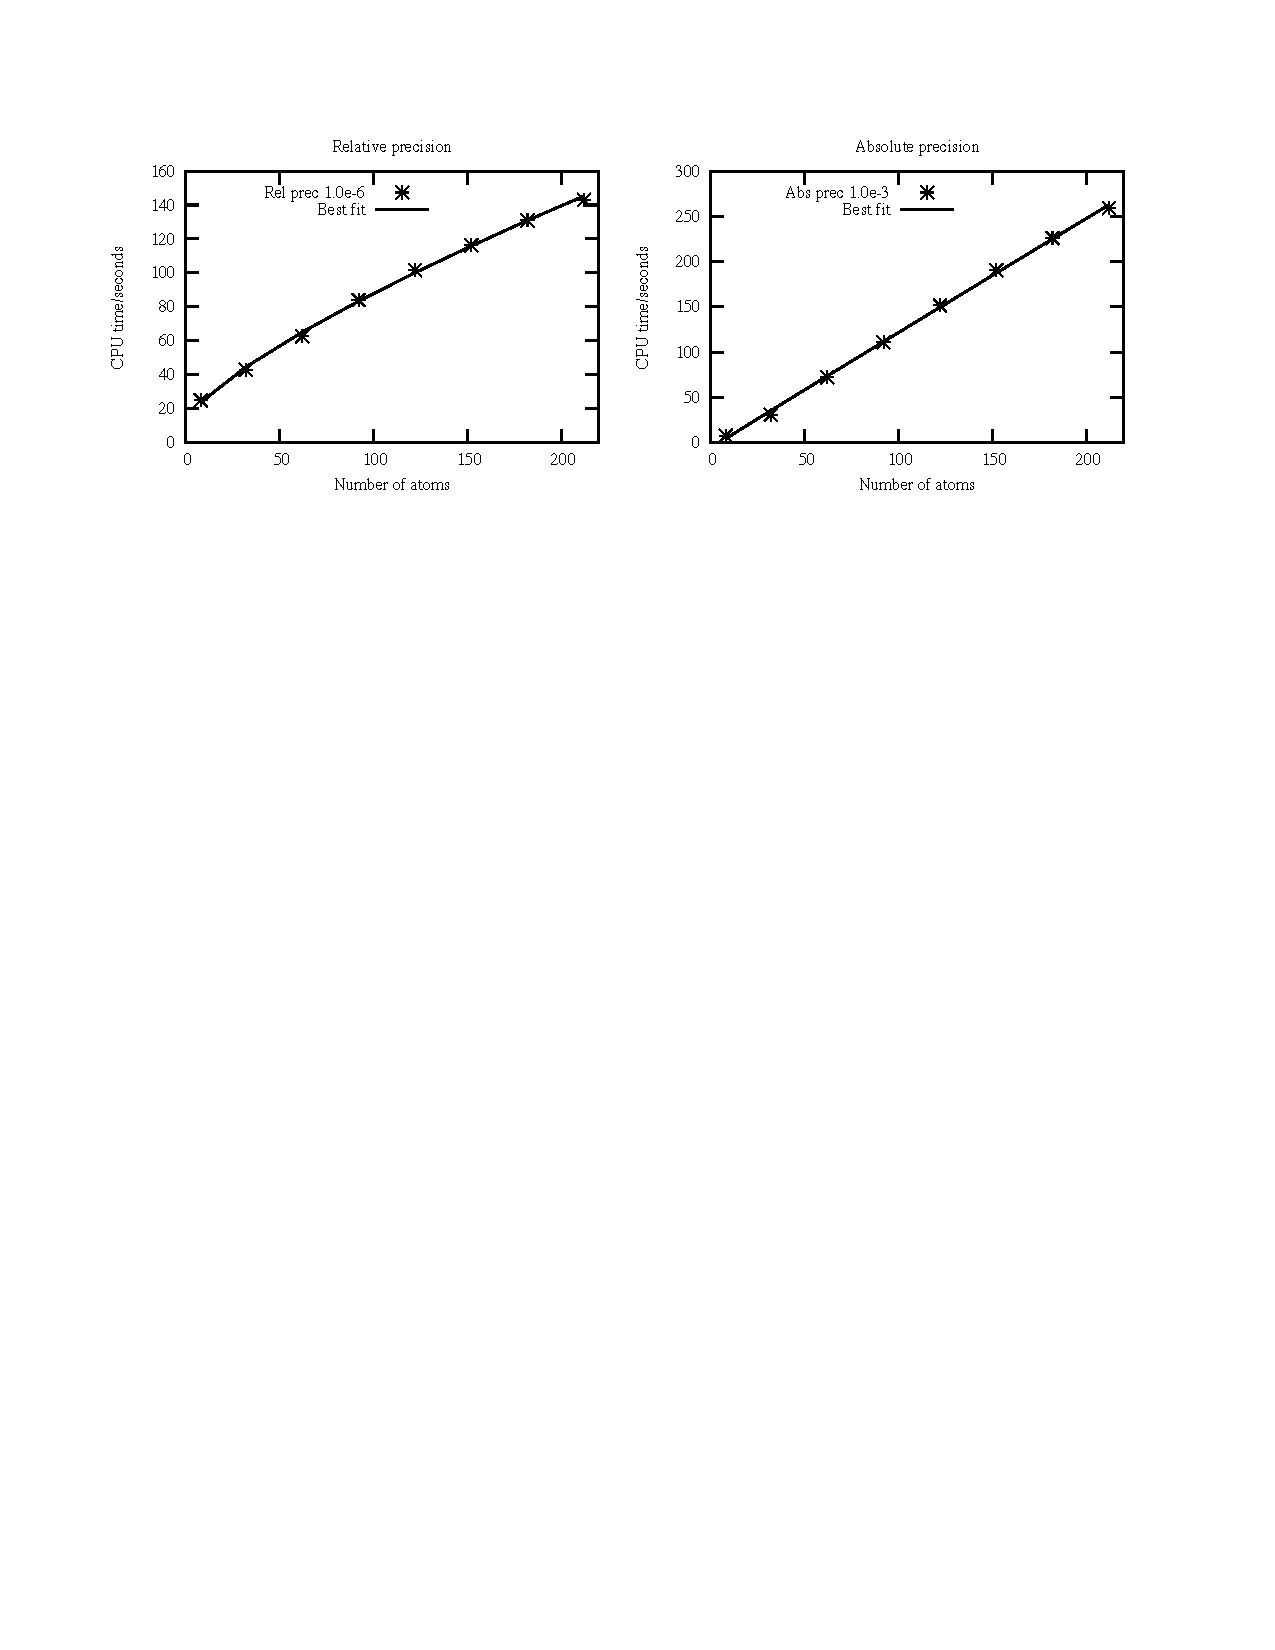
\includegraphics[scale=0.6, clip, viewport = 50 550 540 730]{figures/linearScaling.pdf}
    %\end{center}
%\end{frame}



%%\begin{frame}
    %\frametitle{Parallel programming}
    %Why parallel processing?
    %\begin{itemize}
	%\item	To get more processing power
	%\item	To get more available memory
	%\item	Future $\rightarrow$ \emph{more} processors rather than faster
    %\end{itemize}
    %\ \\
    %\ \\
    %\ \\
    %\pause
    %Parallelization means
    %\begin{itemize}
	%\item	\textbf{distributing work} among available processors
	%\item	\textbf{syncronizing} distributed work
	%\item	\textbf{distributing data} among available memory
	%\item	\textbf{communicating} distributed data
    %\end{itemize}
%\end{frame}

%\begin{frame}
    %\frametitle{Shared memory (OpenMP)}
    %\begin{columns}
    %\begin{column}[b]{0.45\linewidth}
	%Pros
	%\begin{itemize}
	    %\item Relatively simple implementation
	    %\item Quick way to good performance
	    %\item No communication
	    %\item Simple load balance
	%\end{itemize}
	%\ \\
	%\ \\
	%\pause
	%Cons
        %\begin{itemize}
	    %\item Small to medium scale parallelization
	    %\item Limited memory
	    %\item Race conditions
	    %\item Tedious debugging (Heisenbugs)
	%\end{itemize}
	%\ \\
	%\ \\
    %\end{column}
    %\begin{column}[b]{0.4\linewidth}
	%\only<3>{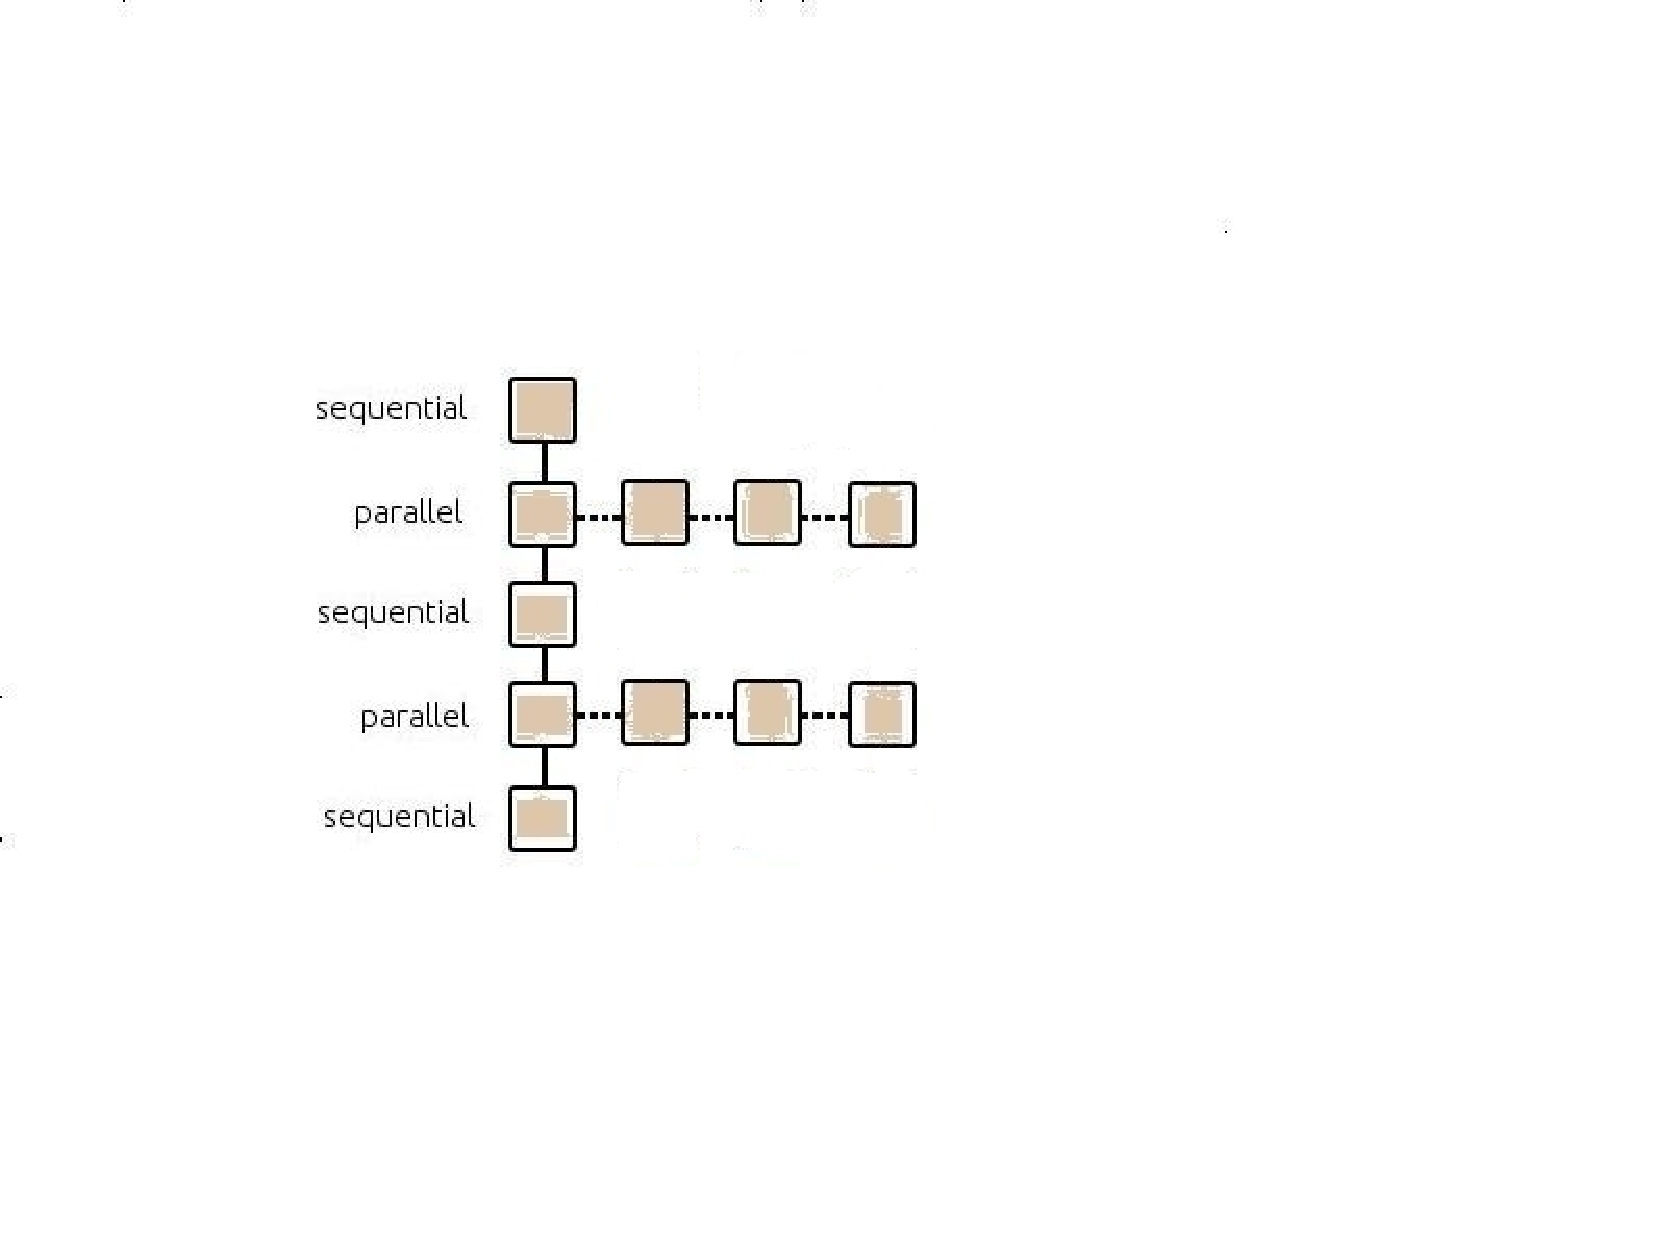
\includegraphics[viewport = 120 160 460 450, clip, scale=0.4]{figures/parallel_OMP.pdf}}
	%\ \\
	%\ \\
	%\ \\
	%\ \\
    %\end{column}
    %\end{columns}
%\end{frame}

%\begin{frame}
    %\frametitle{Distributed memory (MPI)}
    %\begin{columns}
    %\begin{column}[b]{0.45\linewidth}
	%Pros
	%\begin{itemize}
	    %\item Large scale parallelization
	    %\item Extensive memory
	%\end{itemize}
	%\ \\
	%\ \\
	%\ \\
	%\ \\
	%\pause
	%Cons
	%\begin{itemize}
	    %\item Complicated implementation
	    %\item User specified work/data decomposition 
	    %\item User specified communication
	    %\item Difficult to load balance
	    %\item Communication overhead
	%\end{itemize}
    %\end{column}
    %\begin{column}[b]{0.4\linewidth}
	%\only<3>{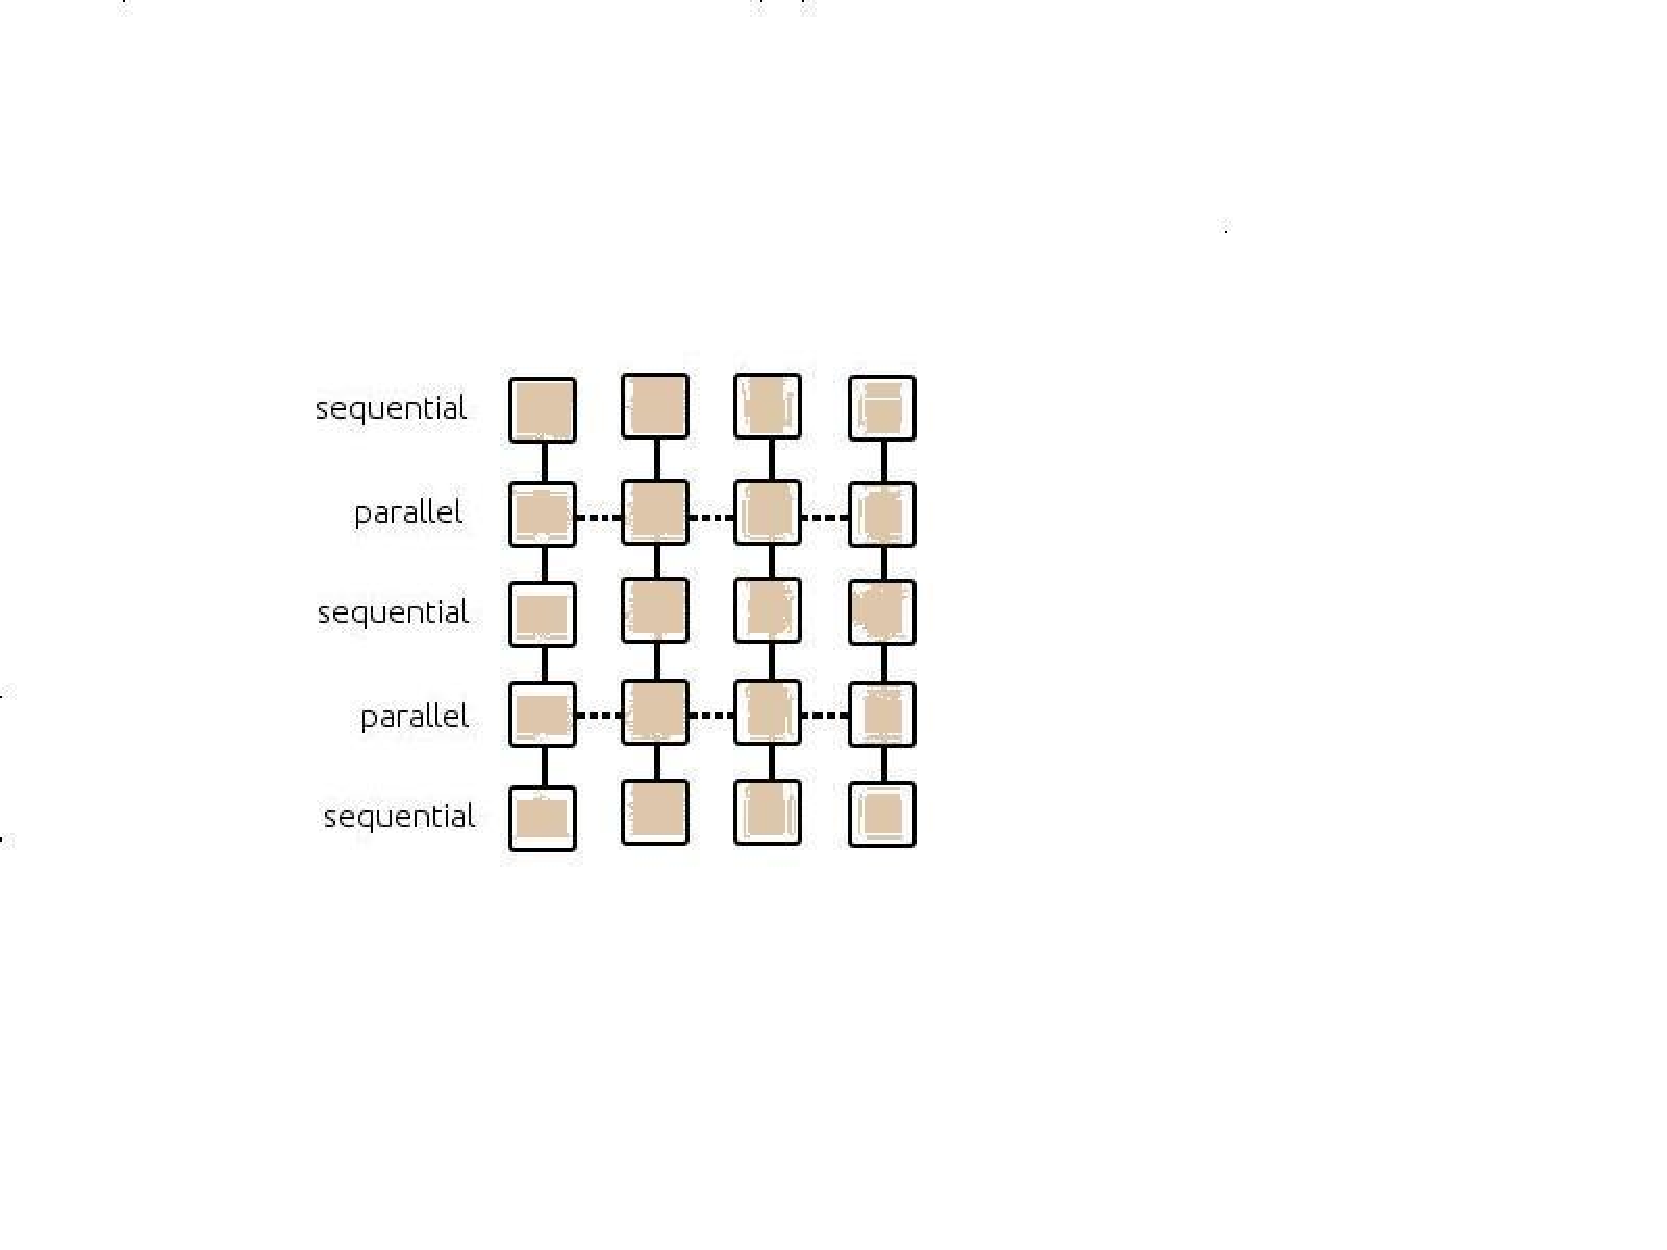
\includegraphics[viewport = 120 160 460 450, clip, scale=0.4]{figures/parallel_mpi_2.pdf}}
	%\ \\
	%\ \\
	%\ \\
    %\end{column}
    %\end{columns}
%\end{frame}

%\begin{frame}
    %\frametitle{Parallel efficiency}
    %\begin{center}
    %\only<1>{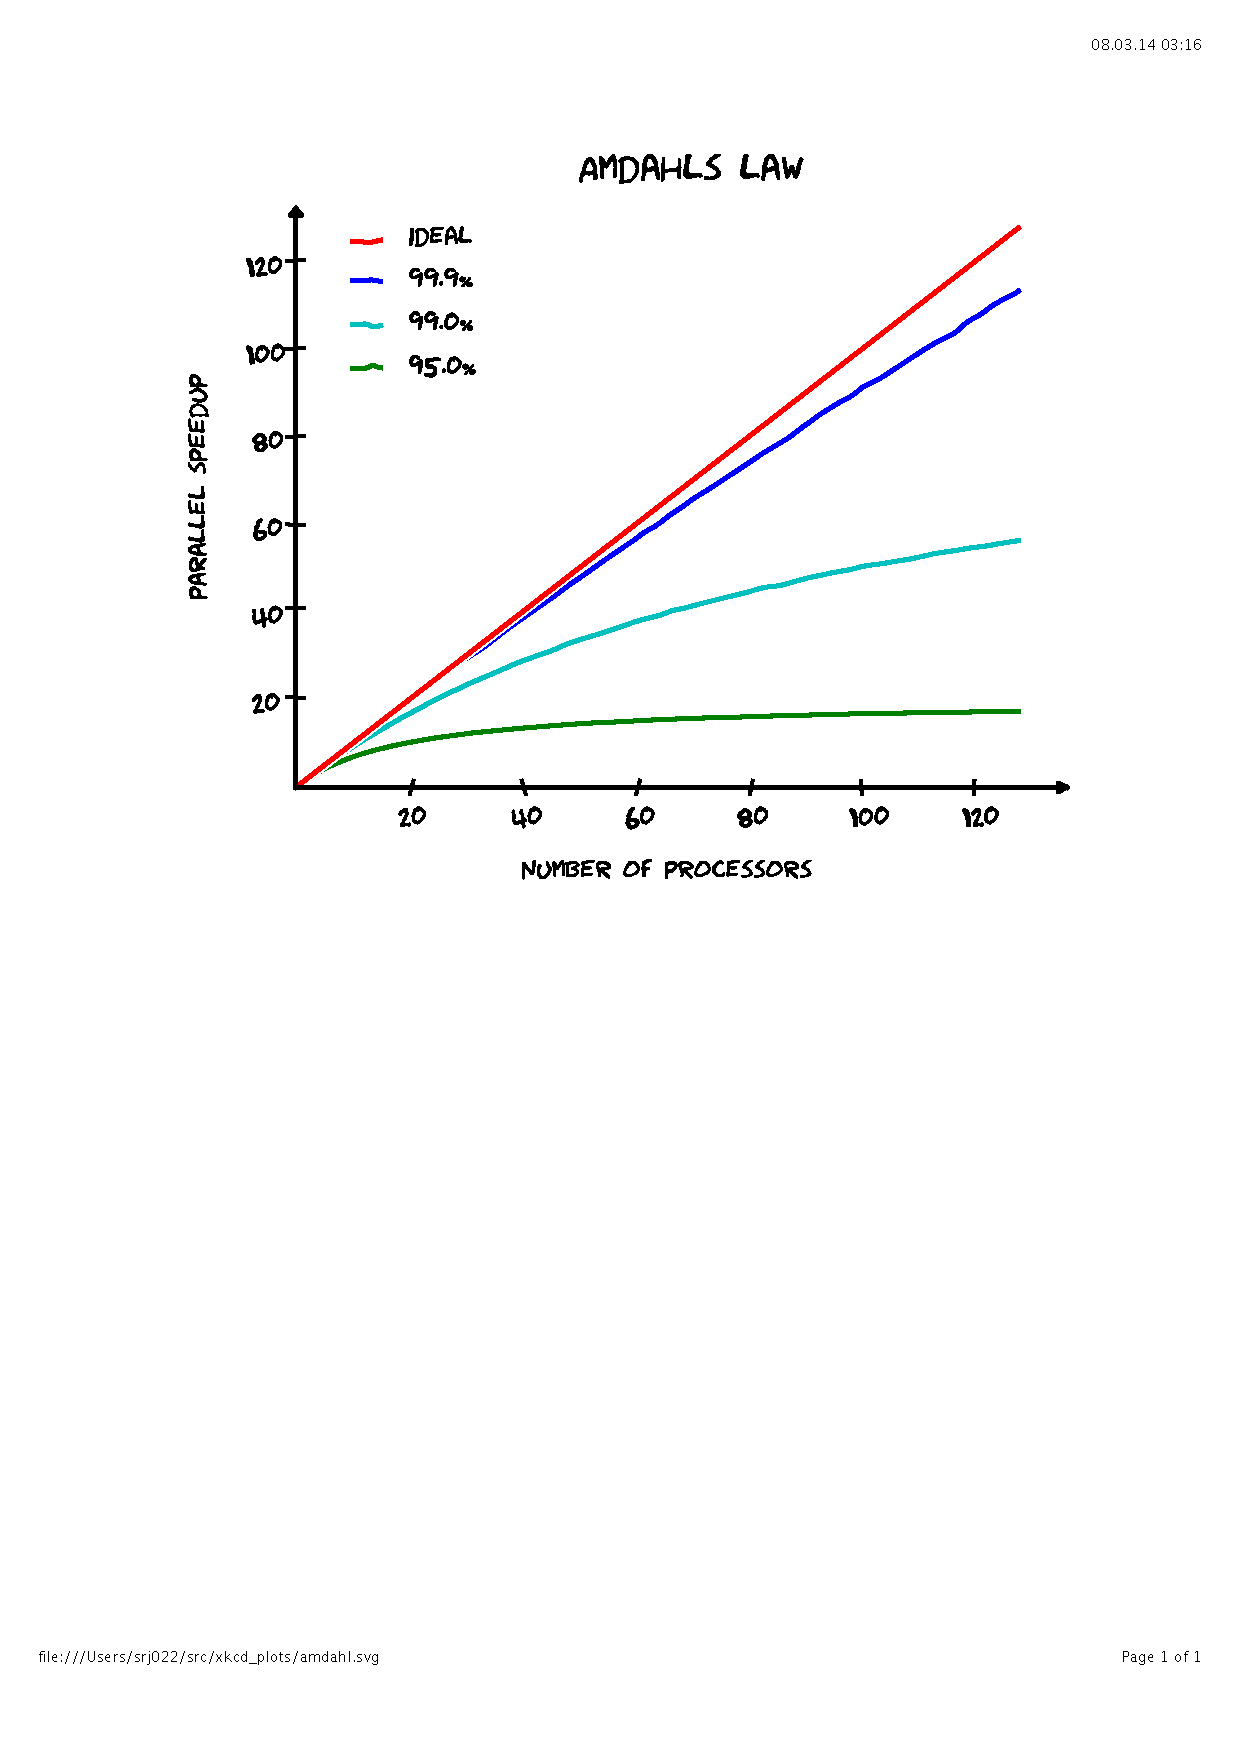
\includegraphics[clip, viewport = 50 250 550 800, scale=0.5]{figures/amdahl.pdf}}
    %\only<2>{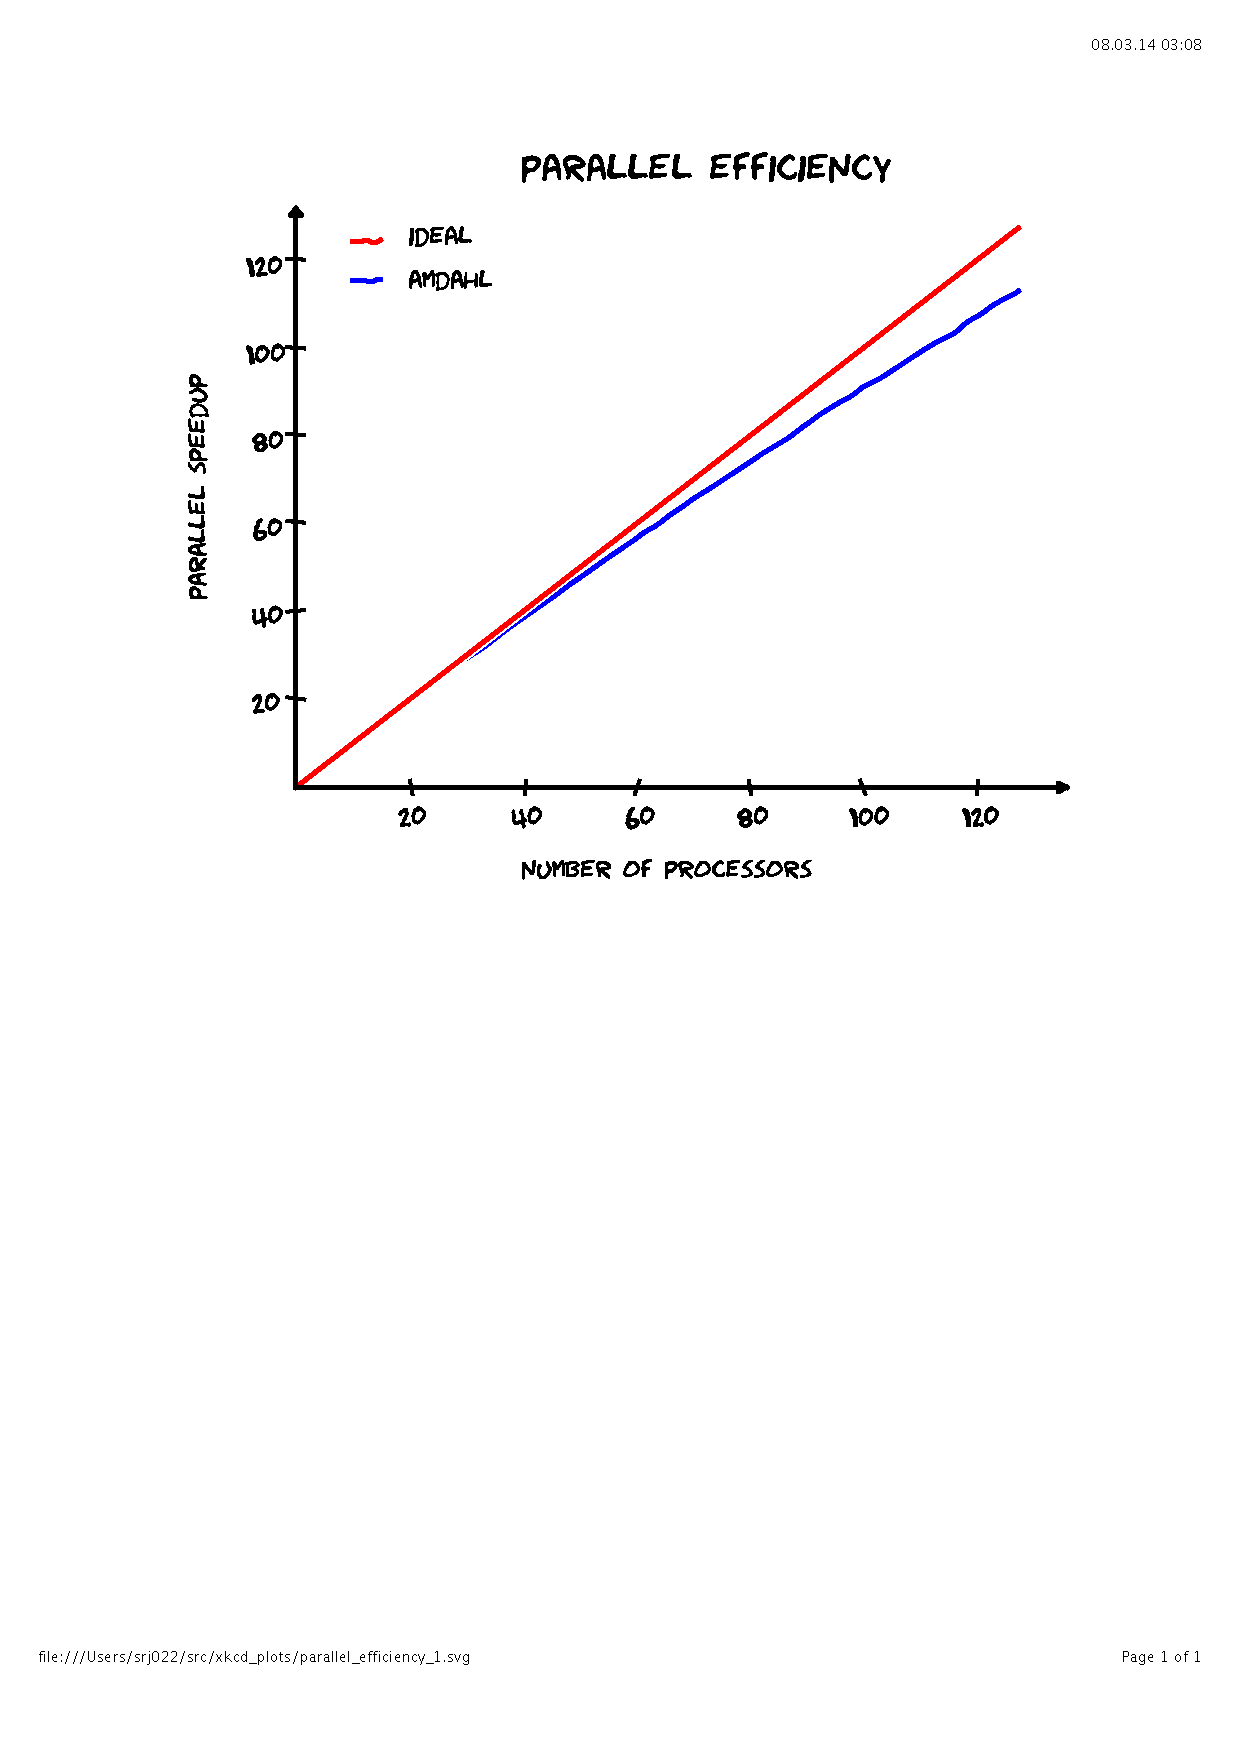
\includegraphics[clip, viewport = 50 250 550 800, scale=0.5]{figures/parallel_efficiency_1.pdf}}
    %\only<3>{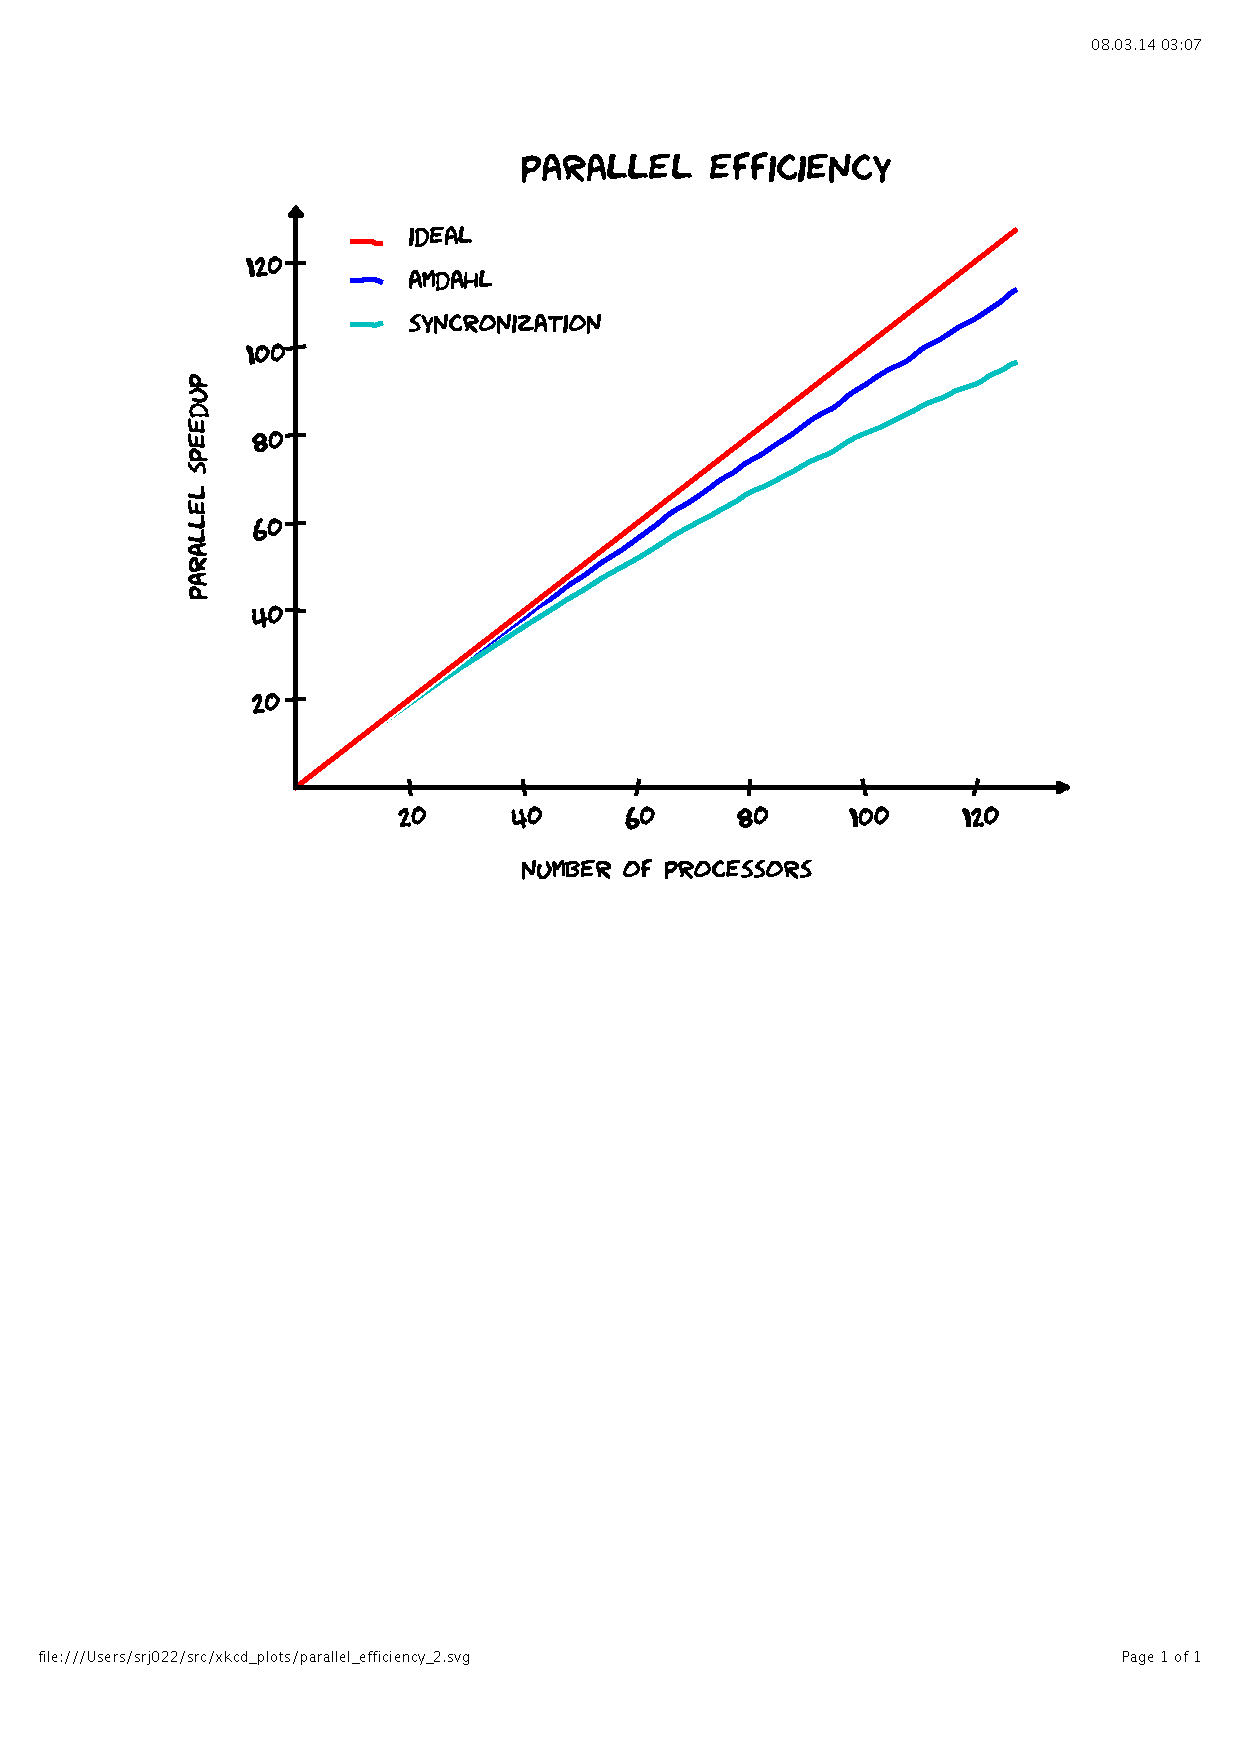
\includegraphics[clip, viewport = 50 250 550 800, scale=0.5]{figures/parallel_efficiency_2.pdf}}
    %\only<4>{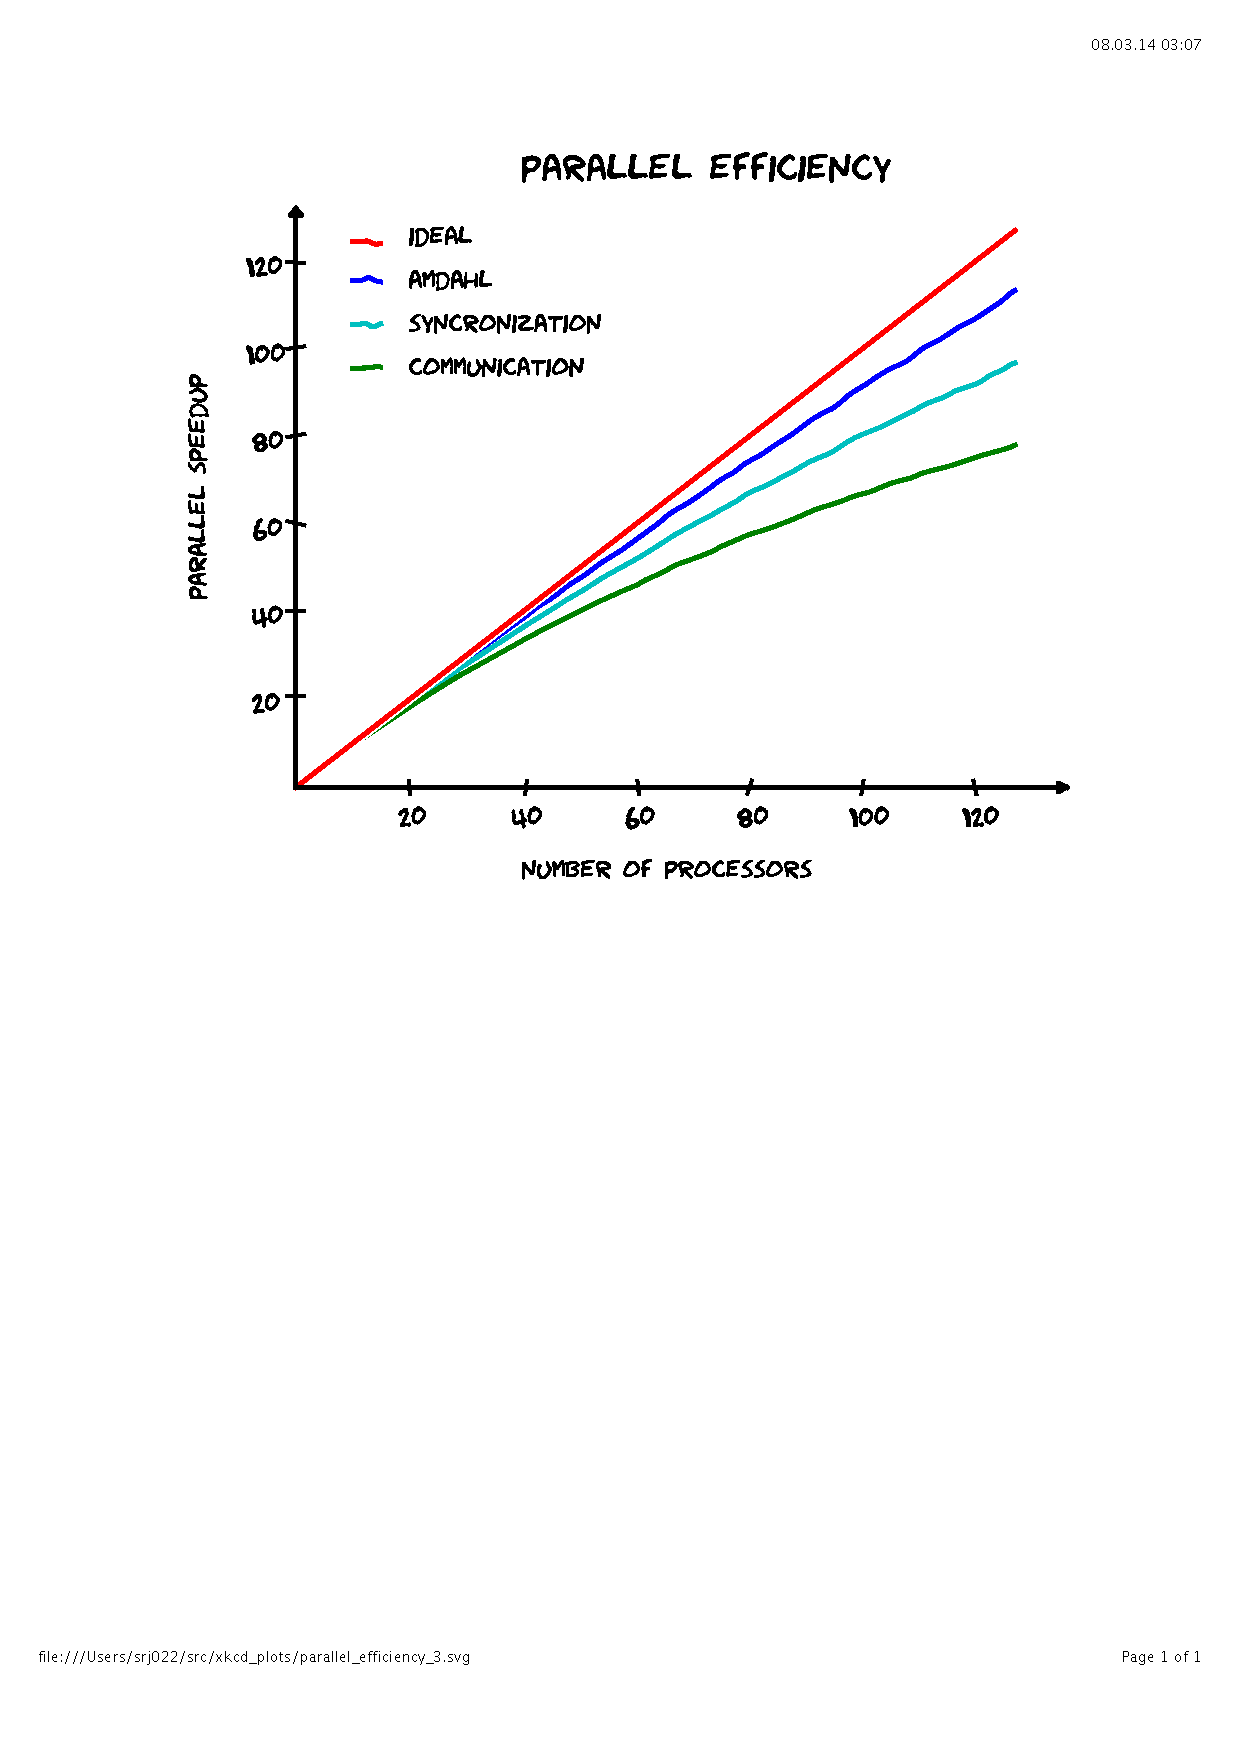
\includegraphics[clip, viewport = 50 250 550 800, scale=0.5]{figures/parallel_efficiency_3.pdf}}
    %\end{center}
%\end{frame}

\begin{frame}
    \frametitle{Parallelization}
    \begin{columns}
    \begin{column}{.5\textwidth}
	\ \ \ \ \textbf{Shared memory using OpenMP}
	\begin{itemize}
	    \item All CPUs have access to the \textbf{full} grid
	    \item No communication needed
	    \item Small scale parallelization ($<50$ CPUs)
	    \item Work (grid cells) dynamically distributed
	\end{itemize}
    \end{column}
    \begin{column}{.5\textwidth}
	\ \ \ \ \textbf{Distributed memory using MPI}
	\begin{itemize}
	    \item Each CPU has access to a \textbf{local} part of the grid
	    \item Communication required
	    \item Large scale parallelization ($>1000$ CPUs)
	    \item Work (grid cells) distributed \it{a priori}
	\end{itemize}
    \end{column}
    \end{columns}
    \ \\
    \ \\
    \ \\
    \ \\
    \centering
    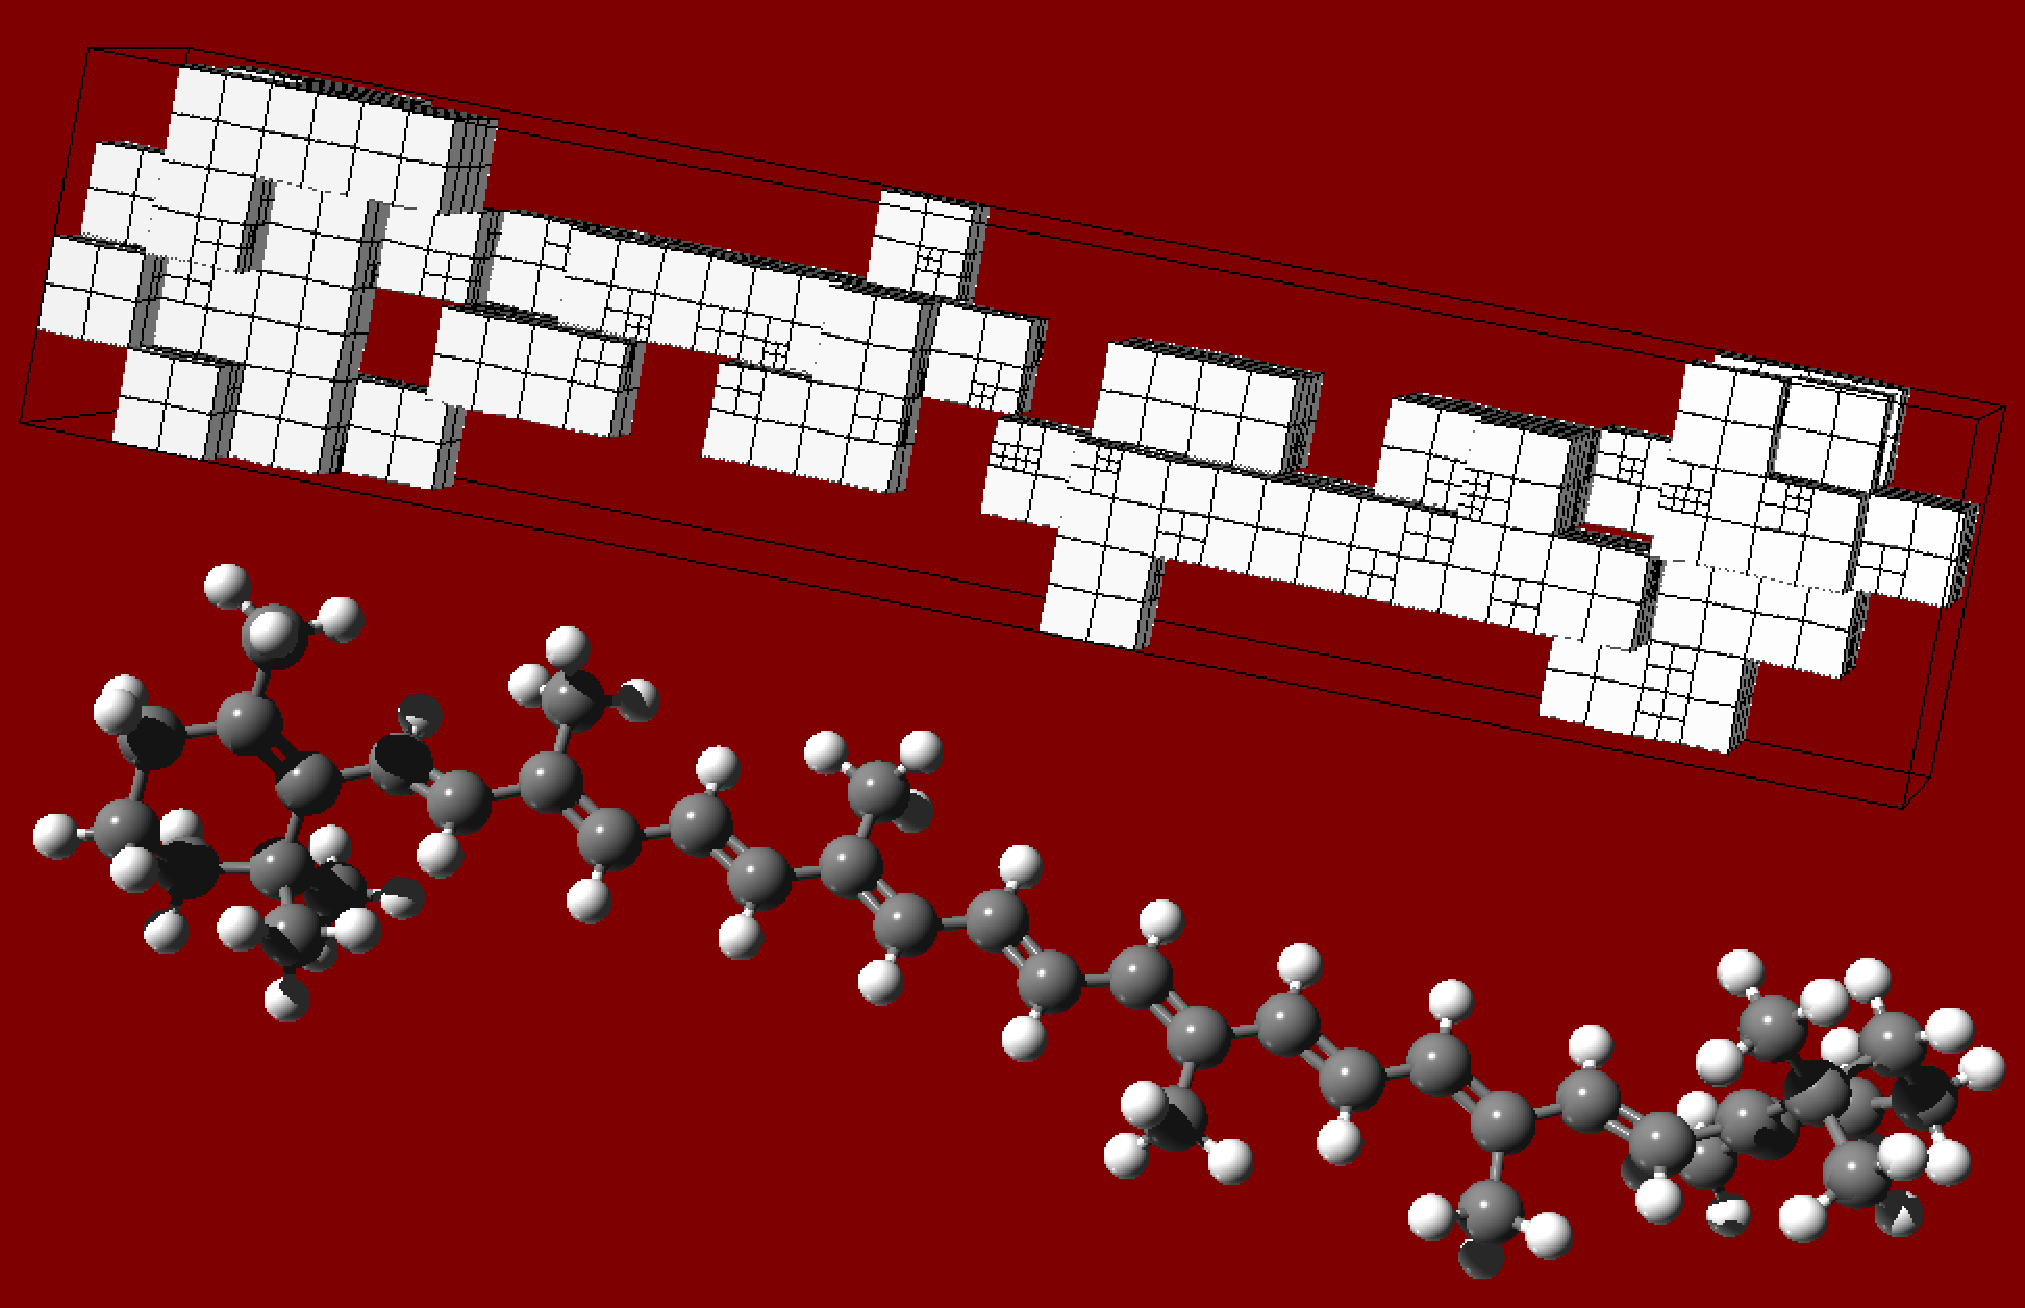
\includegraphics[angle=0, scale=0.2]{figures/caroteneGrid.pdf}
\end{frame}

\begin{frame}
    \frametitle{Linear scaling and parallel performance}
    \begin{columns}
    \begin{column}{.10\textwidth}
    \ \\
    \end{column}
    \begin{column}{.40\textwidth}
    \centering
    Electrostatic potential calculated to a relative precision of $\epsilon=10^{-6}$
    for diamond fragments
    \begin{equation}
	\nonumber
	C_{(2n+3)(n+2)(n+1)/6}H_{2(n+2)(n+1)}
    \end{equation}
    \ \\
    \ \\
    \ \\
    Fitted curve
    \begin{equation}
	\nonumber
	t(n) = 11.6 + 1.84n^{0.805}
    \end{equation}
    \end{column}
    \begin{column}{.50\textwidth}
	\begin{figure}
	    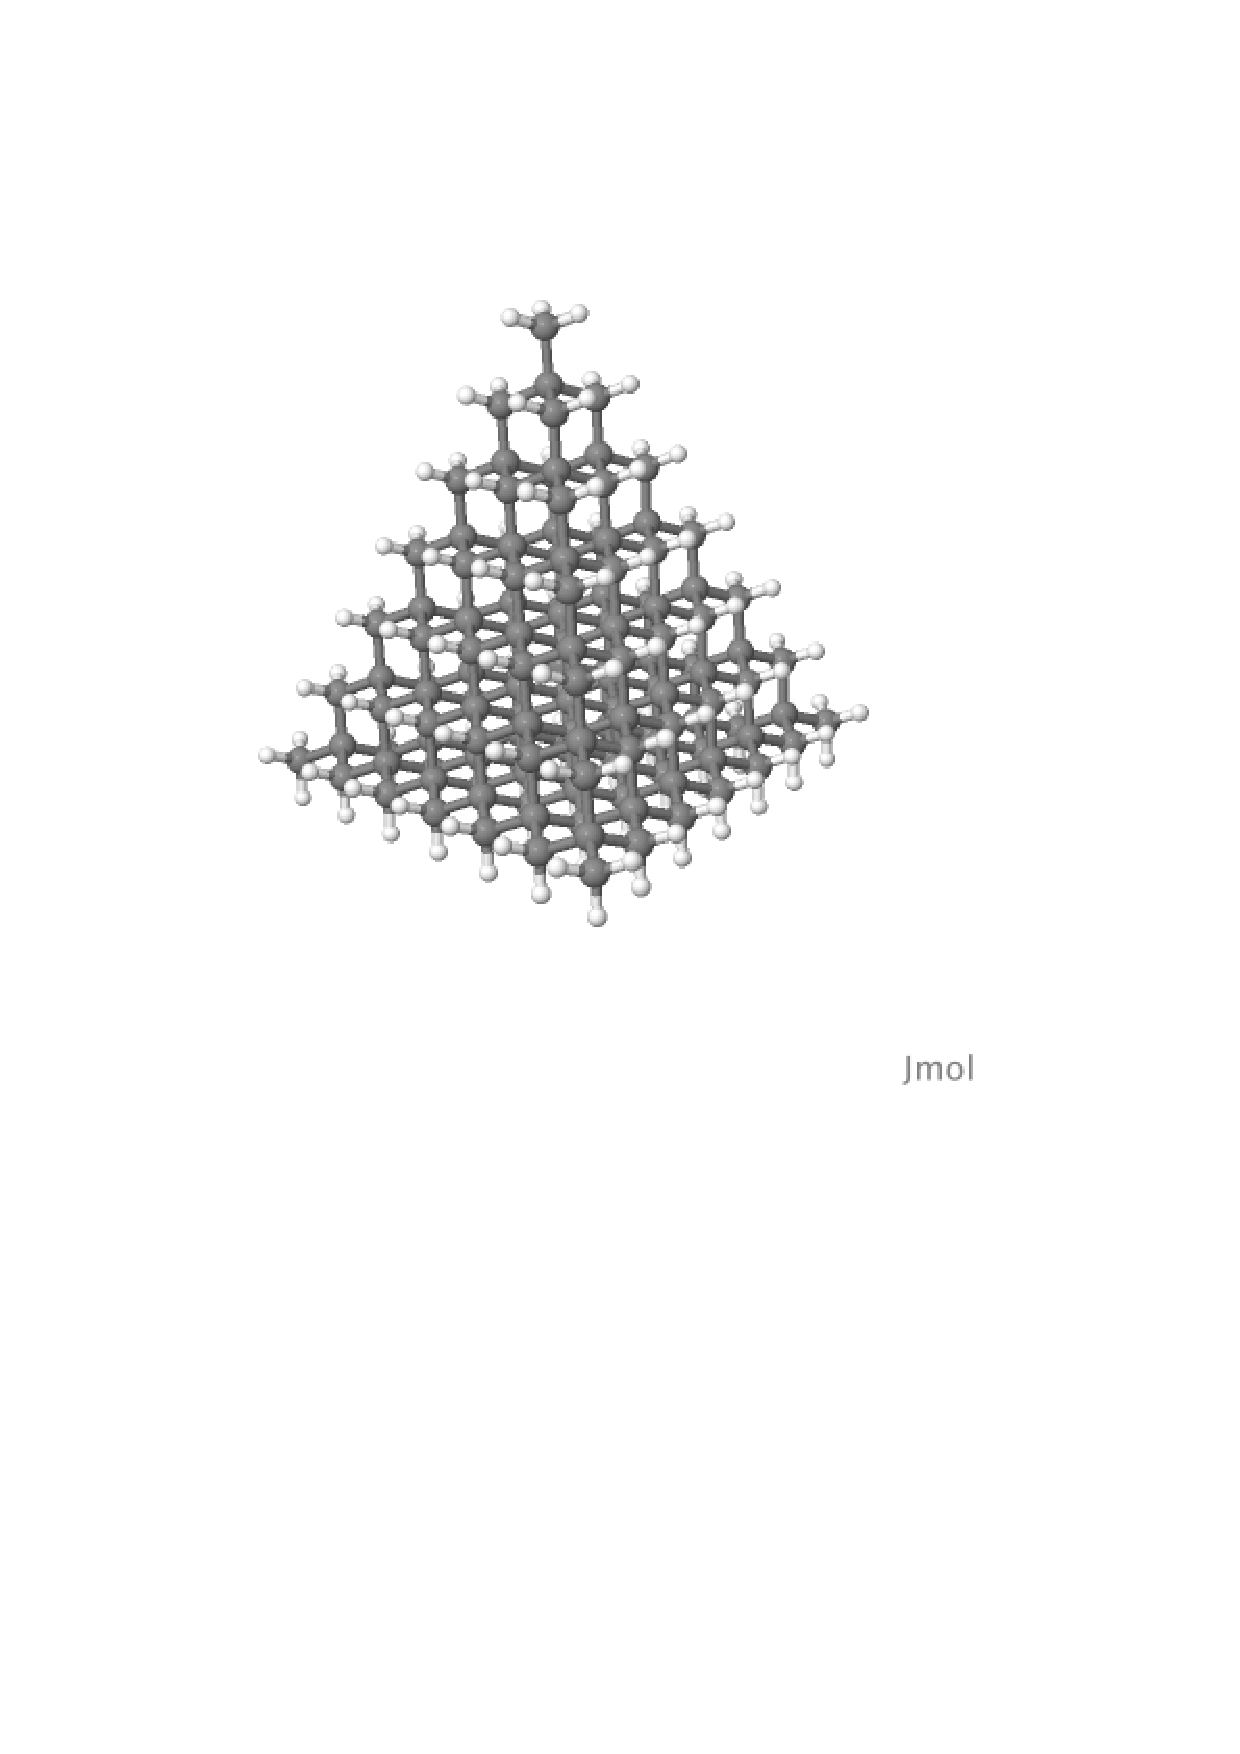
\includegraphics[scale=0.25, clip, viewport = 10 390 500 720]{figures/diamond.pdf}
	\end{figure}
    \end{column}
    \end{columns}    
    \begin{center}
	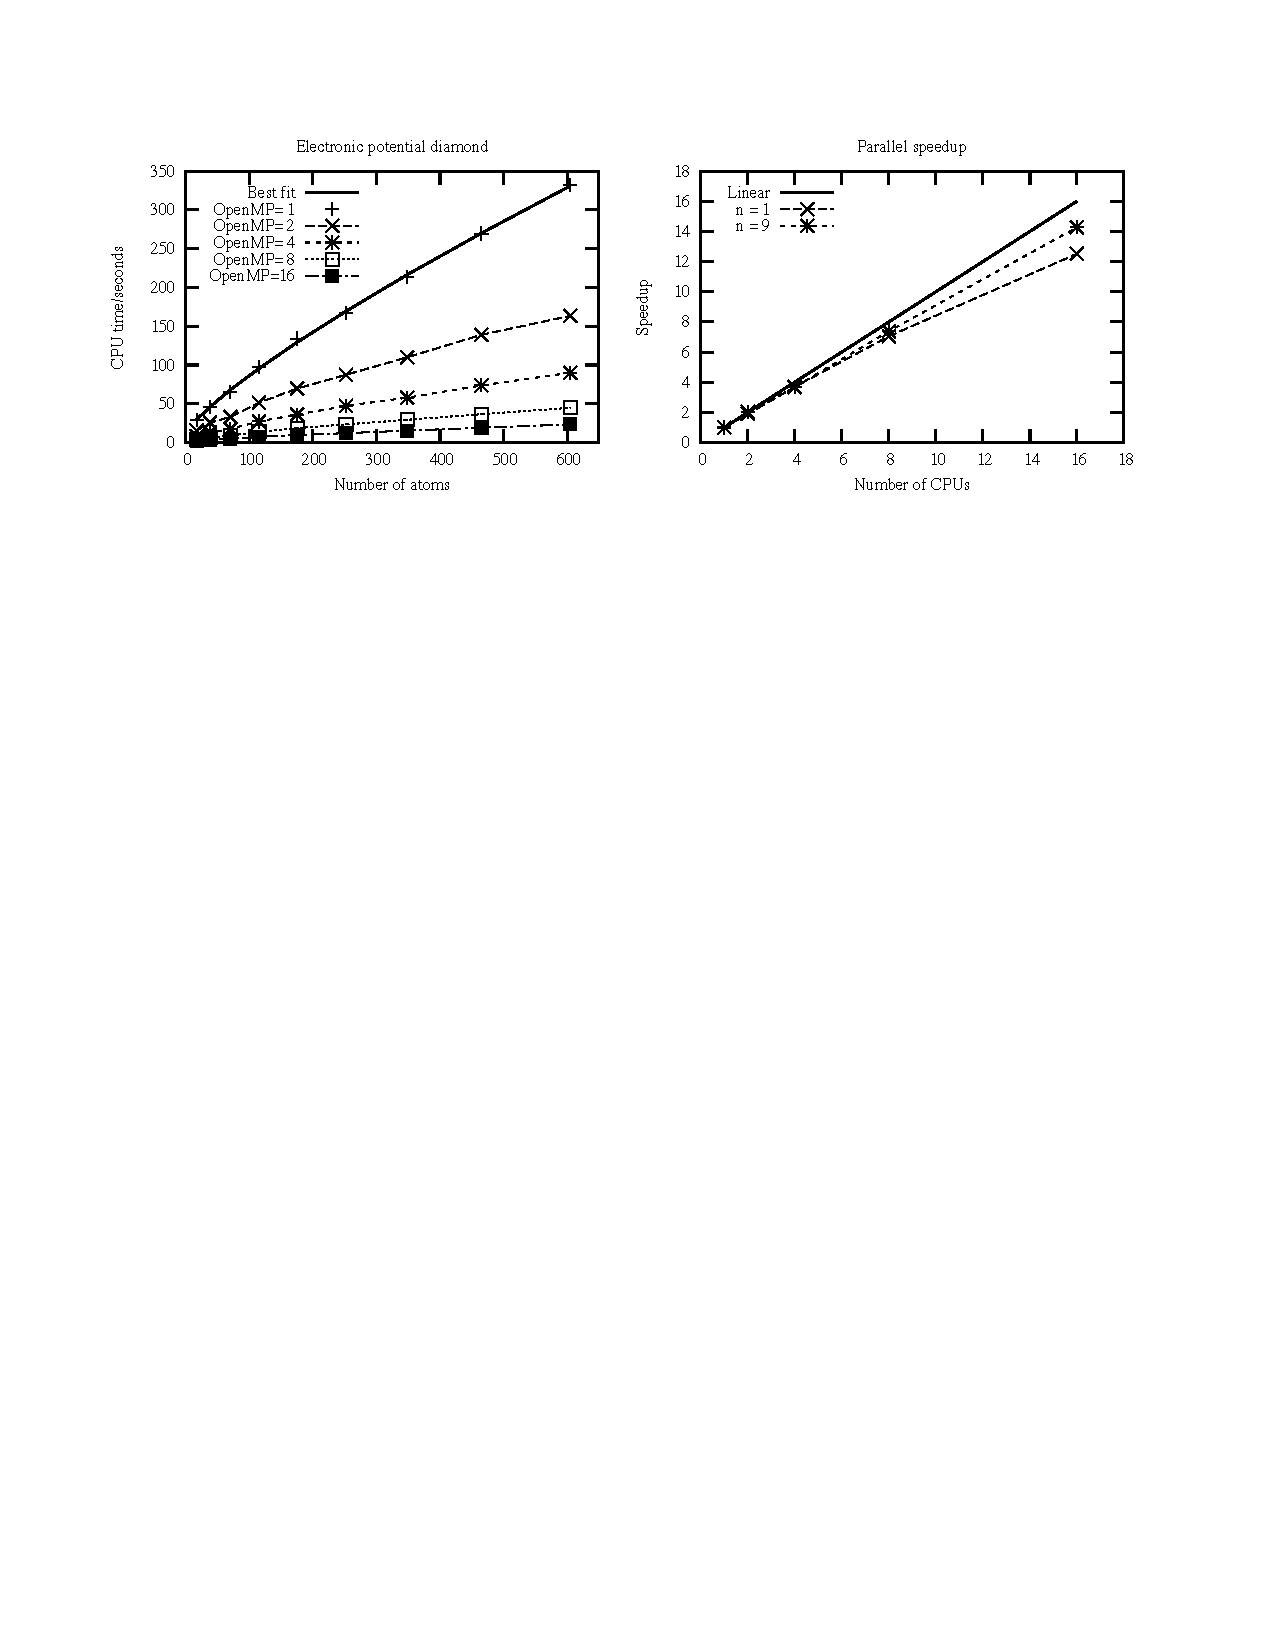
\includegraphics[scale=0.6, clip, viewport = 50 550 540 730]{figures/ompScaling.pdf}
    \end{center}
\end{frame}

\begin{frame}
    \frametitle{Linear scaling and parallel performance}
    \centering
    Wall clock computation time in seconds for parallel calculation of electronic potential\\
    of diamond fragments using pure OpenMP and hybrid MPI/OpenMP strategies.\\
    \begin{table}
    \tiny
    \begin{tabular}{cccrrrrrrrrr}
	\hline
	\hline                                                                           
	\multicolumn{3}{c}{Number of CPUs}&
	\multicolumn{9}{c}{Diamond system $n$ in $C_{(2n+3)(n+2)(n+1)/6}H_{2(n+2)(n+1)}$}\\
	MPI&OMP&TOT	&1	&2	&3	&4	&5	&6	&7	&8	&9	\\
	\hline
	   &   &   	&	&      	&	&	&	&	&	&	&	\\
	  1&  1&  1	& 29.4	& 46.2 	& 64.7 	& 97.8  &133.9  &166.8  &213.4  &269.4  &332.0  \\
	  1&  2&  2	& 15.5	& 25.5 	& 33.0 	& 51.3  & 69.5  & 87.2  &110.0  &138.9  &163.4  \\
	  1&  4&  4	&  8.0 	& 12.8 	& 17.4 	& 27.0  & 36.1  & 47.3  & 57.8  & 73.7  & 90.1  \\
	  1&  8&  8	&  4.2 	&  6.5 	&  8.8 	& 13.9  & 18.6  & 23.5  & 29.4  & 36.7  & 45.0  \\
	  1& 16& 16	&  2.4 	&  3.5 	&  4.7 	&  7.5  &  9.6  & 12.2  & 15.4  & 19.1  & 23.3  \\
	   %&   &   	&      	&      	&    	&    	&    	&	&	&	&	\\
	  %2&  1&  2	& 17.9 	& 28.4 	& 35.8 	& 59.2  & 81.6  & 93.0  &121.7  &147.5  &176.5  \\
	  %4&  1&  4	& 10.1 	& 16.3 	& 21.2 	& 32.5  & 51.6  & 53.8  & 60.8  & 85.3  &100.7  \\
	  %8&  1&  8	&  6.1 	&  9.4 	& 11.8 	& 19.9  & 25.6  & 28.0  & 35.4  & 43.7  & 50.7  \\
	 %16&  1& 16	&  5.0 	&  6.2 	&  8.2 	& 12.4  & 15.0  & 17.3  & 23.0  & 26.1  & 31.3  \\
	 %32&  1& 32	&  3.6 	&  4.2 	&  5.4 	&  9.5  &  9.2  & 10.9  & 14.1  & 16.8  & 20.0  \\
	 %64&  1& 64	&  3.1 	&  3.9 	&  4.3 	&  6.5  &  6.6  &  7.4  & 10.3  & 11.4  & 13.4  \\
	%128&  1&128	&  5.2 	&  5.7 	&  6.4 	&  7.6  &  7.8  &  8.8  & 10.9  & 10.9  & 11.9  \\
	   %&   &   	&      	&      	&      	& 	& 	& 	& 	& 	&	\\
	  2& 16& 32	&  1.5 	&  2.2 	&  2.9 	&  4.8  &  6.0  &  7.0  &  9.6  & 11.4  & 13.7  \\
	  4& 16& 64	&  1.1 	&  1.6 	&  2.0 	&  3.2  &  4.3  &  4.7  &  6.3  &  7.3  &  7.9  \\
	  8& 16&128	&  1.0 	&  1.4 	&  1.8 	&  2.9  &  3.3  &  3.8  &  4.8  &  5.9  &  6.4  \\
	 16& 16&256	&  0.9 	&  1.3 	&  1.6 	&  2.2  &  2.9  &  3.3  &  4.2  &  4.9  &  6.0  \\
	 32& 16&512	&  1.1 	&  1.3 	&  1.5 	&  2.0  &  2.4  &  2.8  &  3.4  &  4.0  &  4.8  \\
	   &   &   	&      	&      	&      	&    	&    	&	&	&	&	\\
	\hline                                                                           
	\hline
    \end{tabular}
    \end{table}
    \ \\
    \ \\
    \begin{itemize}
	\item Computation time can be pushed down to a few seconds for all systems
	\item Efficient OpenMP implementation (90\% at 16 CPUs)
	\item Hybrid MPI/OpenMP preferred over pure MPI for a given number of CPUs
    \end{itemize}
\end{frame}



%\begin{frame}
%    \centering
%    \Large{Part III:}\\
%    \ \\
%    \ \\
%    \centering
%    \Large{Real-space Density Functional Theory with\\ Localized Orbitals and Multiwavelets}
%\end{frame}

%\begin{frame}
%    \frametitle{The molecular Schr\"{o}dinger equation}
%    \ \\
%    \begin{equation}
%	\nonumber
%	\hat{H}\psi = E\psi
%    \end{equation}
%    \ \\
%    \begin{equation}
%	\nonumber
%	\hat{H} =   -\sum_I \frac{\nabla^2}{2M_I} - \sum_i \frac{\nabla^2}{2}
%		    +\sum_{I>J} \frac{Z_IZ_J}{|\boldsymbol{R}_I-\boldsymbol{R}_J|} 
%		    -\sum_{i,I} \frac{Z_I}{|\boldsymbol{r}_i-\boldsymbol{R}_I|} 
%		    +\sum_{i>j} \frac{1}{|\boldsymbol{r}_i-\boldsymbol{r}_j|} 
%    \end{equation}
%    \ \\
%    \ \\
%    \ \\
%    \centering
%    For an $N$-particle problem, the wave function is $3N$-dimensional
%    \begin{equation}
%	\nonumber
%	\psi = \psi(\boldsymbol{r}_1,\boldsymbol{r}_2,\dots,\boldsymbol{r}_N)
%    \end{equation}
%    \ \\
%    \ \\
%    \ \\
%    \pause
%    \centering
%    $\beta$-Carotene ($C_{40}H_{56}$) has 296 electrons and an 888-dimensional wave function!
%    \only<1>{
%    \begin{center}
%    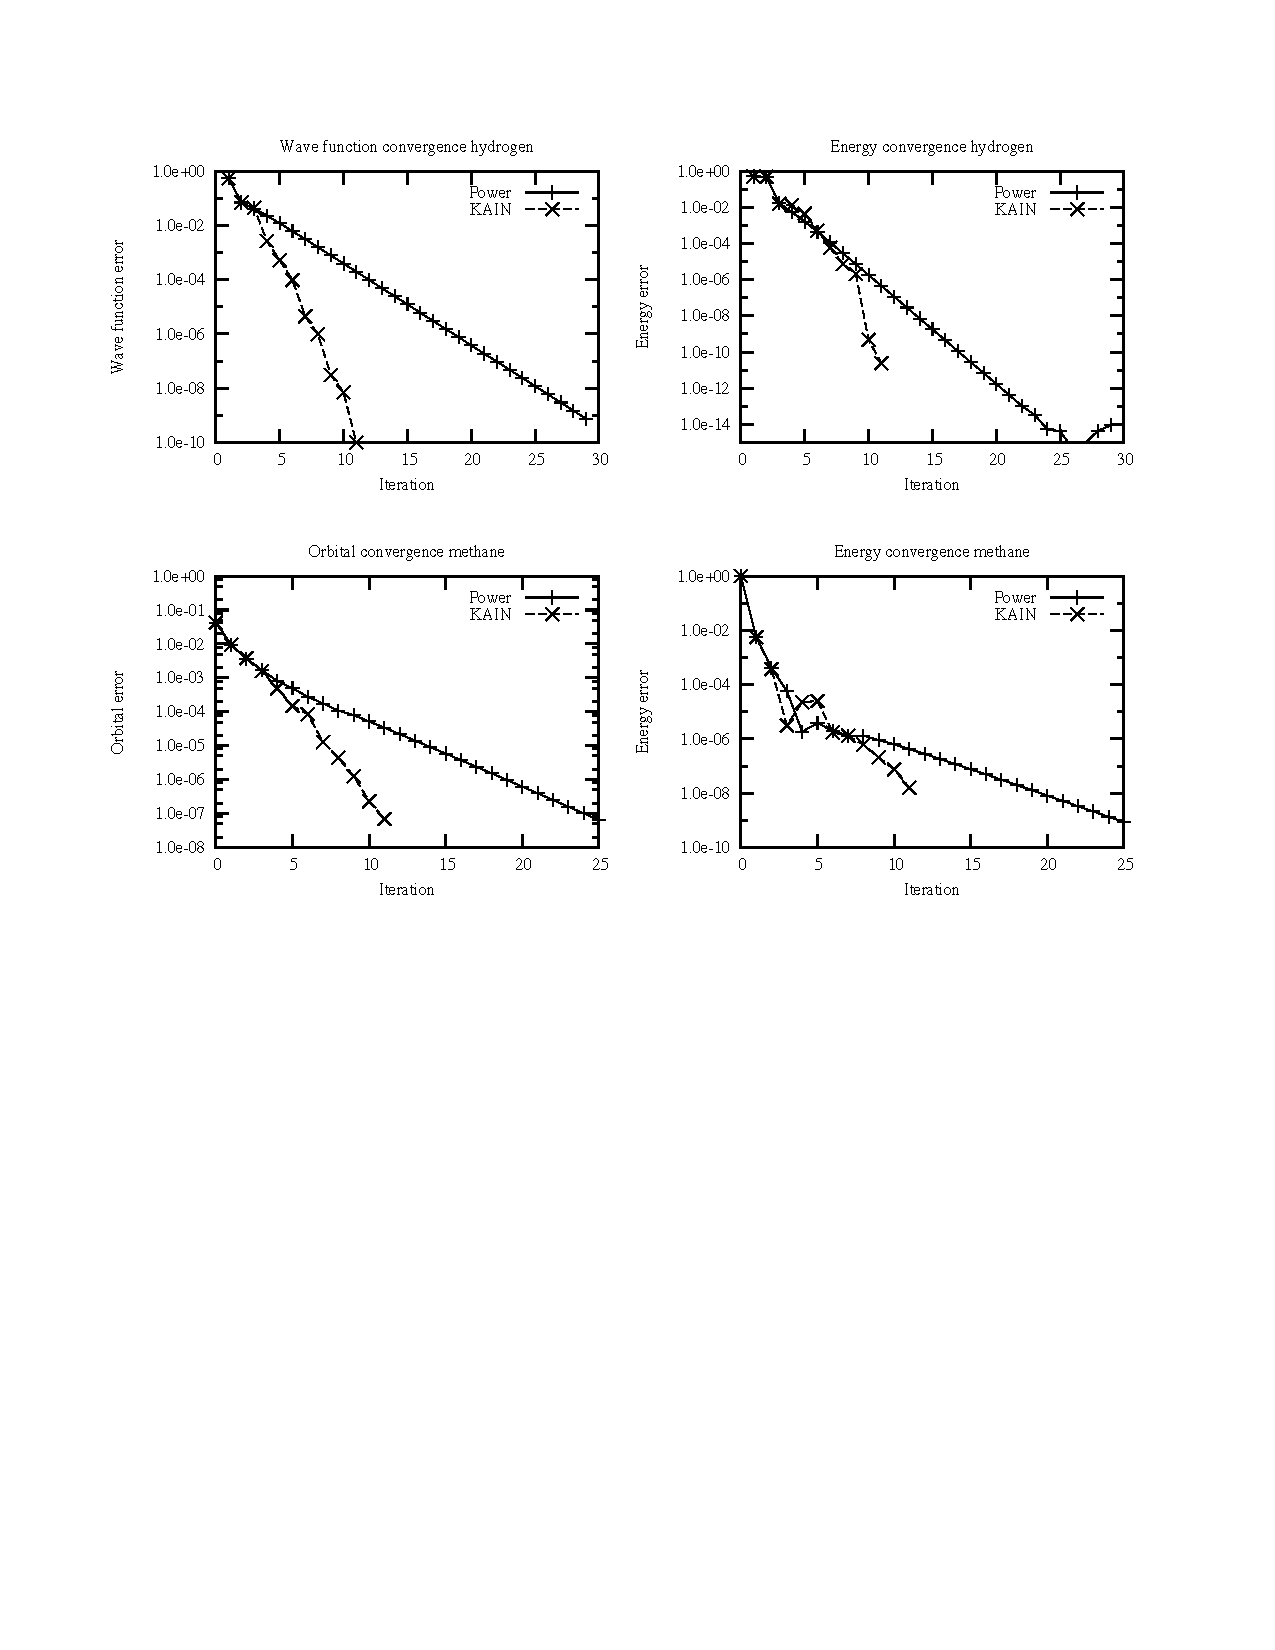
\includegraphics[scale=0.3, clip, viewport = 0 0 900 280]{figures/convergence.pdf}
%    \end{center}
%    }
%    \only<2>{
%    \begin{center}
%    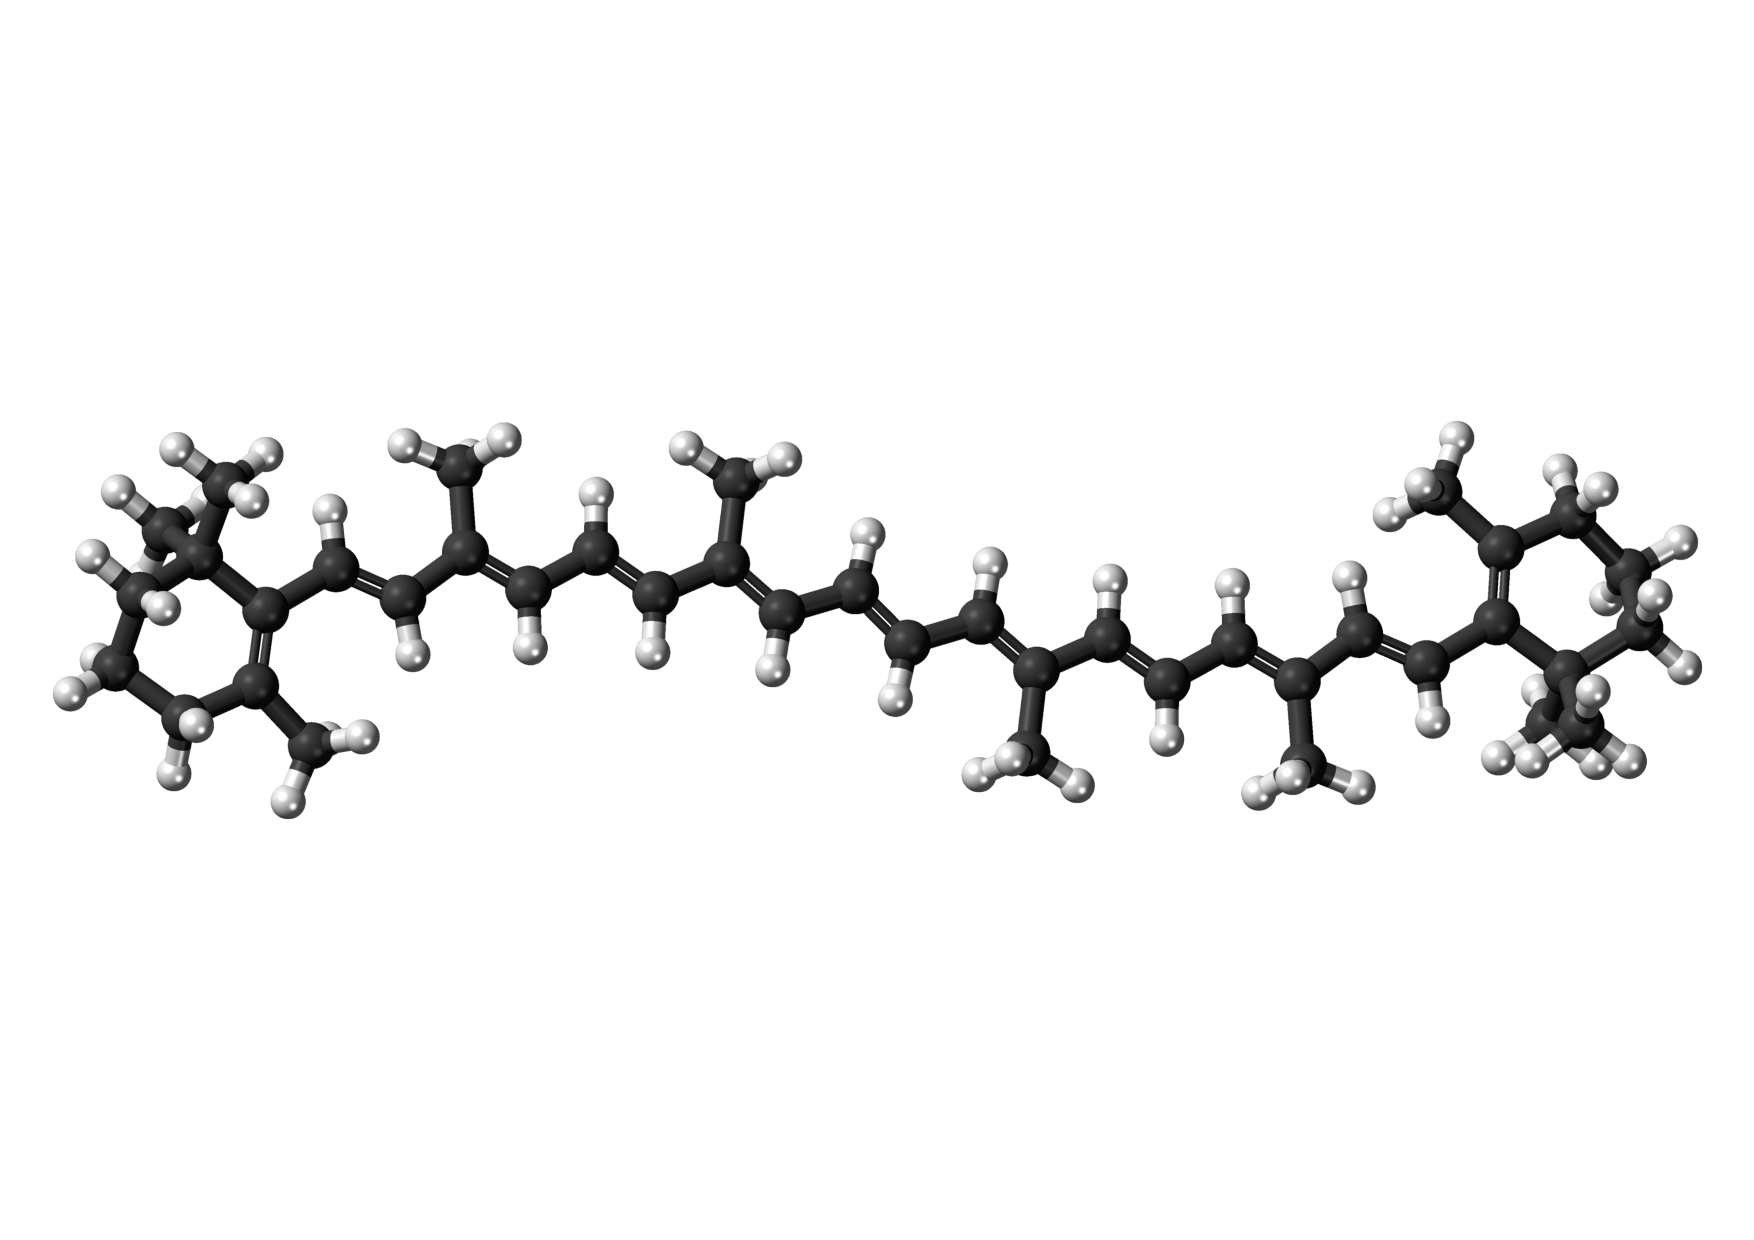
\includegraphics[scale=0.3, clip, viewport = 0 150 900 430]{figures/beta-carotene.pdf}
%    \end{center}
%    }
%\end{frame}

%\begin{frame}
%    \frametitle{Density Functional Theory}
%    \centering
%    Dramatically reduce the dimensionality
%    \begin{equation}
%	\nonumber
%	\rho(\boldsymbol{r}_1) = N \int |\psi(\boldsymbol{r}_1, \boldsymbol{r}_2,\dots,
%	\boldsymbol{r}_N)|^2 d\boldsymbol{r}_2\cdots d\boldsymbol{r}_N
%    \end{equation}
%    \ \\
%    \ \\
%    \ \\
%    \pause
%    Energy expressed as functional of the density
%    \begin{equation}
%	\nonumber
%	E[\rho] = T_s[\rho] + V_{ne}[\rho] + J[\rho] + E_{xc}[\rho]
%    \end{equation}
%    \ \\
%    \ \\
%    \ \\
%    \begin{columns}
%    \begin{column}{.50\textwidth}
%    \centering
%    \pause
%    \textbf{Energy expressions}
%    \begin{align}
%	\nonumber
%	V_{ne}[\rho]	&= \int \rho(\boldsymbol{r})v_{nuc}(\boldsymbol{r})d\boldsymbol{r}\\
%	\nonumber
%			&\\
%	\nonumber
%	J[\rho] &= \frac{1}{2} \int \rho(\boldsymbol{r})v_{el}(\boldsymbol{r})d\boldsymbol{r}\\
%	\nonumber
%			&\\
%	\nonumber
%	E_{xc}[\rho]	&= \int F_{xc}(\rho) d\boldsymbol{r}
%    \end{align}
%    \end{column}
%    \begin{column}{.50\textwidth}
%    \centering
%    \pause
%    \textbf{Potentials}
%    \begin{align}
%	\nonumber
%	v_{nuc}(\boldsymbol{r}) &= -\sum_I\frac{Z_I}{|\boldsymbol{r}-\boldsymbol{R}_I|}\\
%	\nonumber
%			&\\
%	\nonumber
%	v_{el}(\boldsymbol{r}) &= 
%	    \int \frac{\rho(\boldsymbol{r}')}{4\pi|\boldsymbol{r}-\boldsymbol{r}'|} d\boldsymbol{r}'\\
%	\nonumber
%			&\\
%	\nonumber
%	v_{xc}(\boldsymbol{r}) &= \frac{\delta E_{xc}[\rho]}{\delta\rho}
%    \end{align}
%    \end{column}
%    \end{columns}    
%\end{frame}

%\begin{frame}
%    \frametitle{Kohn-Sham DFT}
%    \centering
%    Express density through one-electron orbitals
%    \begin{equation}
%	\nonumber
%	\rho(\boldsymbol{r}) = \sum_i |\phi_i(\boldsymbol{r})|^2
%    \end{equation}
%    \ \\
%    \ \\
%    \ \\
%    \ \\
%    \pause
%    \begin{columns}
%    \begin{column}{.50\textwidth}
%    \centering
%    Kinetic energy
%    \begin{equation}
%	\nonumber
%	T_s[\rho] = -\sum_i \frac{1}{2}\nabla^2\phi_i(\boldsymbol{r})
%    \end{equation}
%    \end{column}
%    \begin{column}{.50\textwidth}
%    \centering
%    Effective potential
%    \begin{equation}
%	\nonumber
%	v_{eff}(\boldsymbol{r}) = v_{nuc}(\boldsymbol{r}) + v_{el}(\boldsymbol{r}) + v_{xc}(\boldsymbol{r})
%    \end{equation}
%    \end{column}
%    \end{columns}
%    \ \\
%    \ \\
%    \ \\
%    \ \\
%    \pause
%    \centering
%    \textbf{The Kohn-Sham equations}
%    \begin{equation}
%	\nonumber
%	\left[-\frac{1}{2}\nabla^2 + v_{eff}(\boldsymbol{r})\right]\phi_i(\boldsymbol{r}) = 
%	\epsilon_i\phi_i(\boldsymbol{r})
%    \end{equation}
%\end{frame}

\begin{frame}
    \frametitle{Computational chemistry}
    \begin{center}
    \only<1>{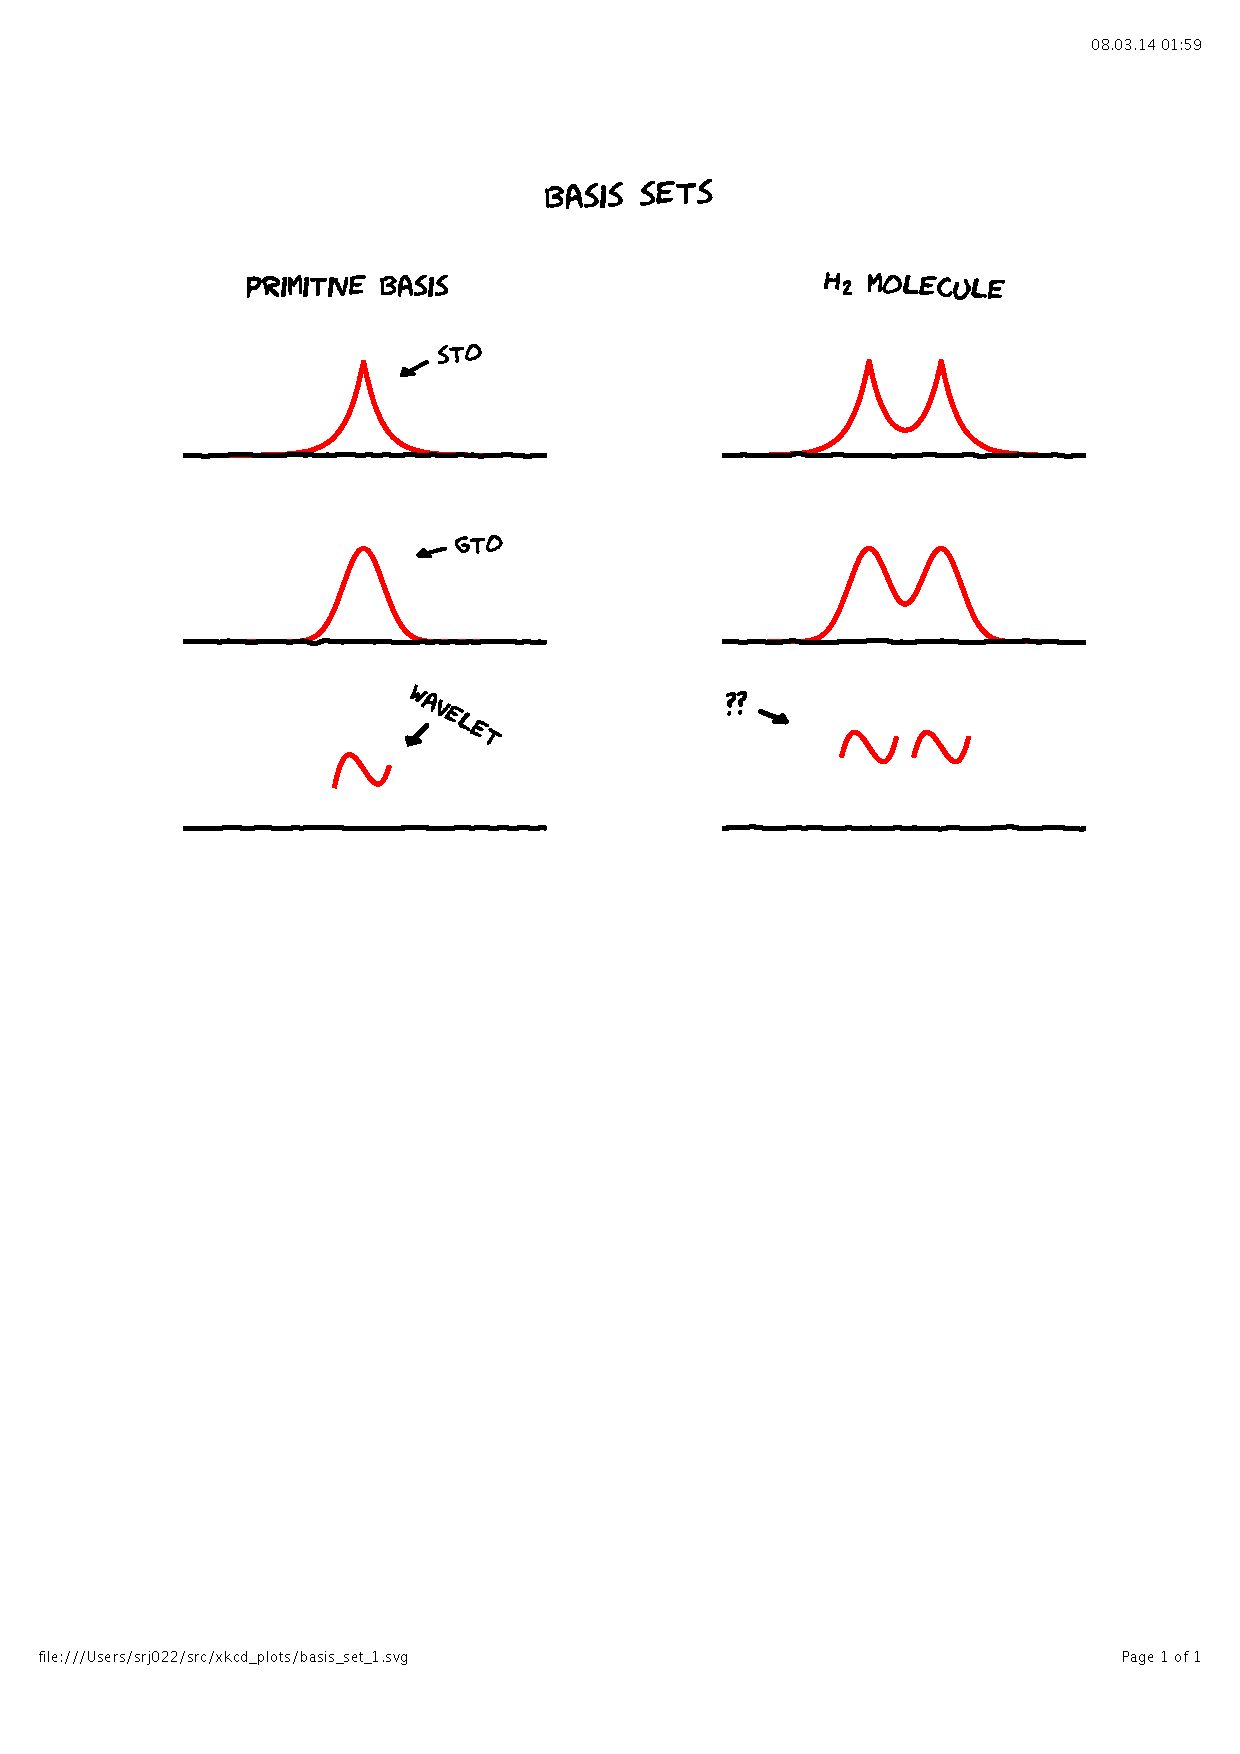
\includegraphics[scale=0.5, clip, viewport = 50 300 550 800]
        {figures/basis_set_1.pdf}}
    \only<2>{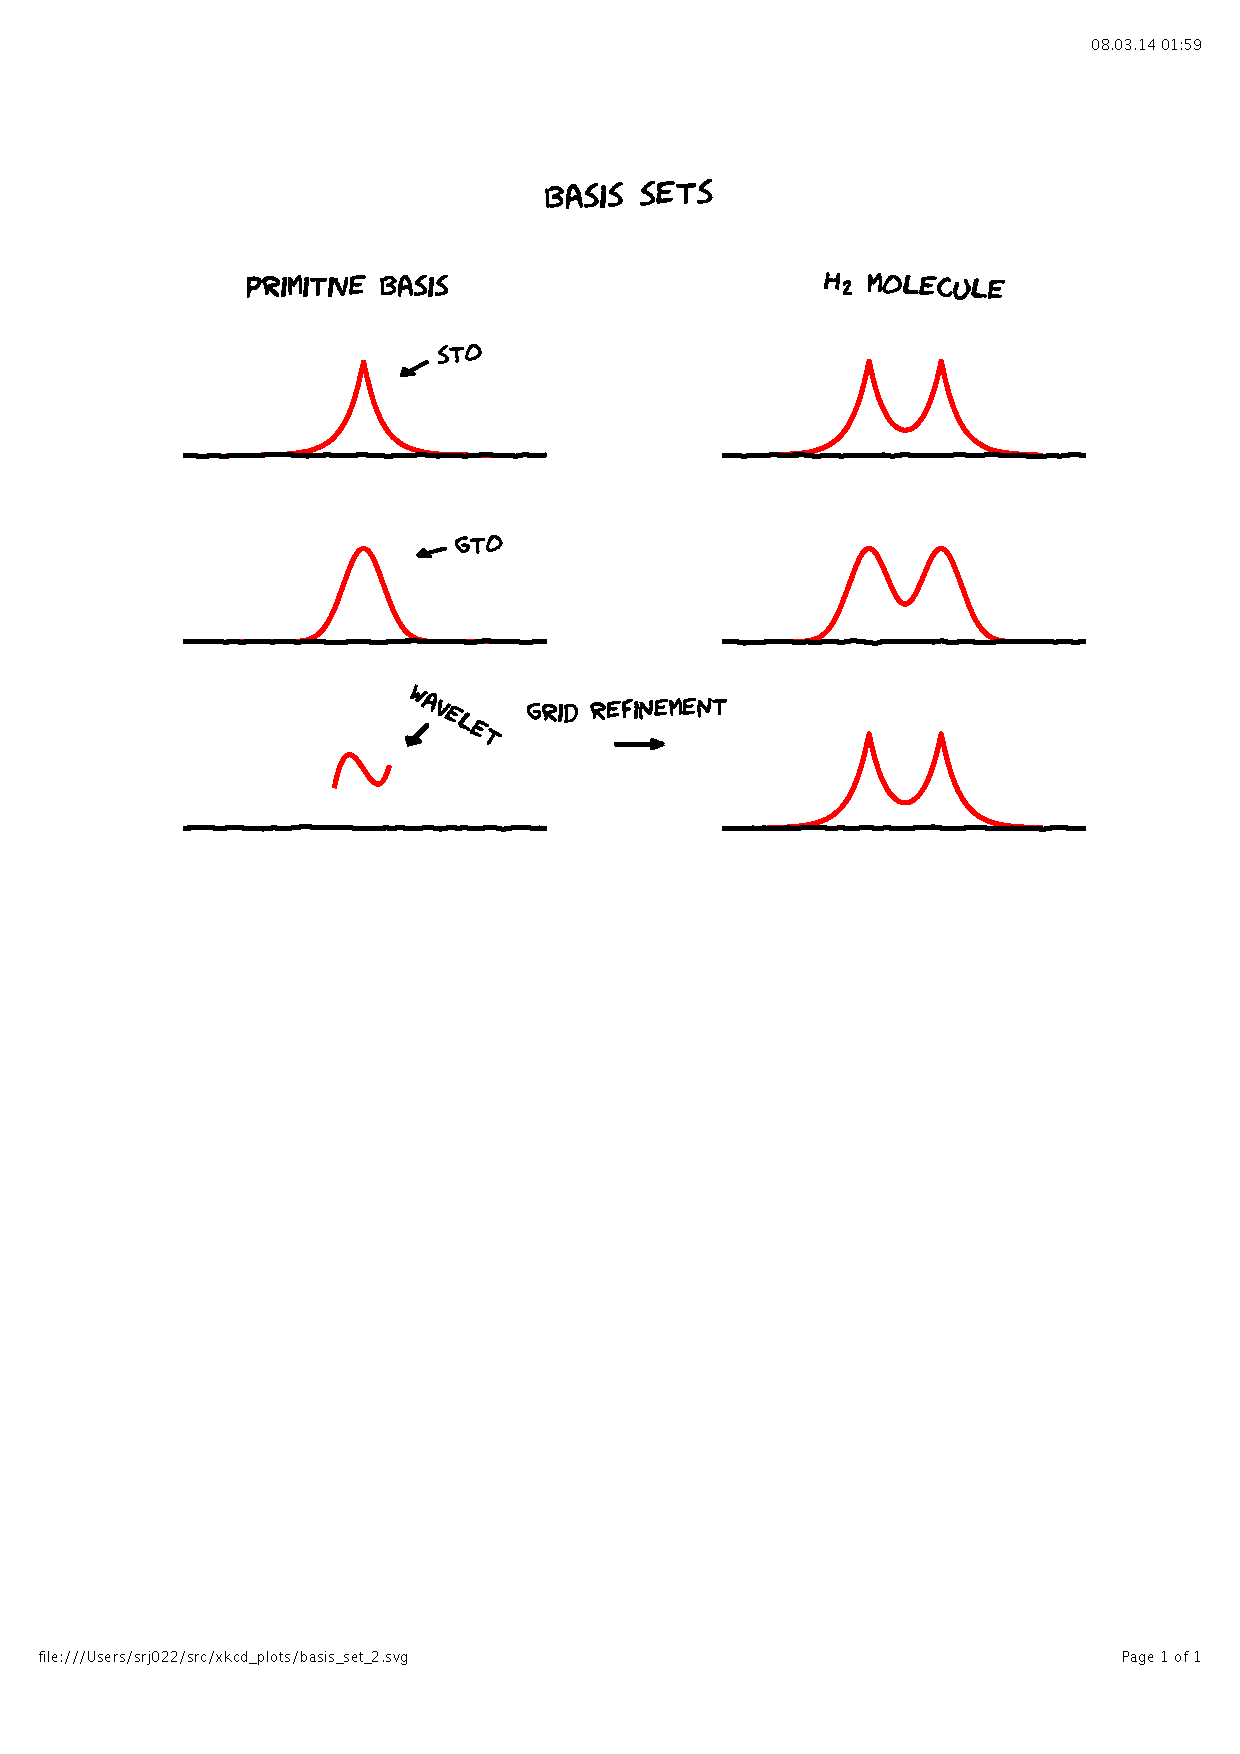
\includegraphics[scale=0.5, clip, viewport = 50 300 550 800]
        {figures/basis_set_2.pdf}}
    \only<3>{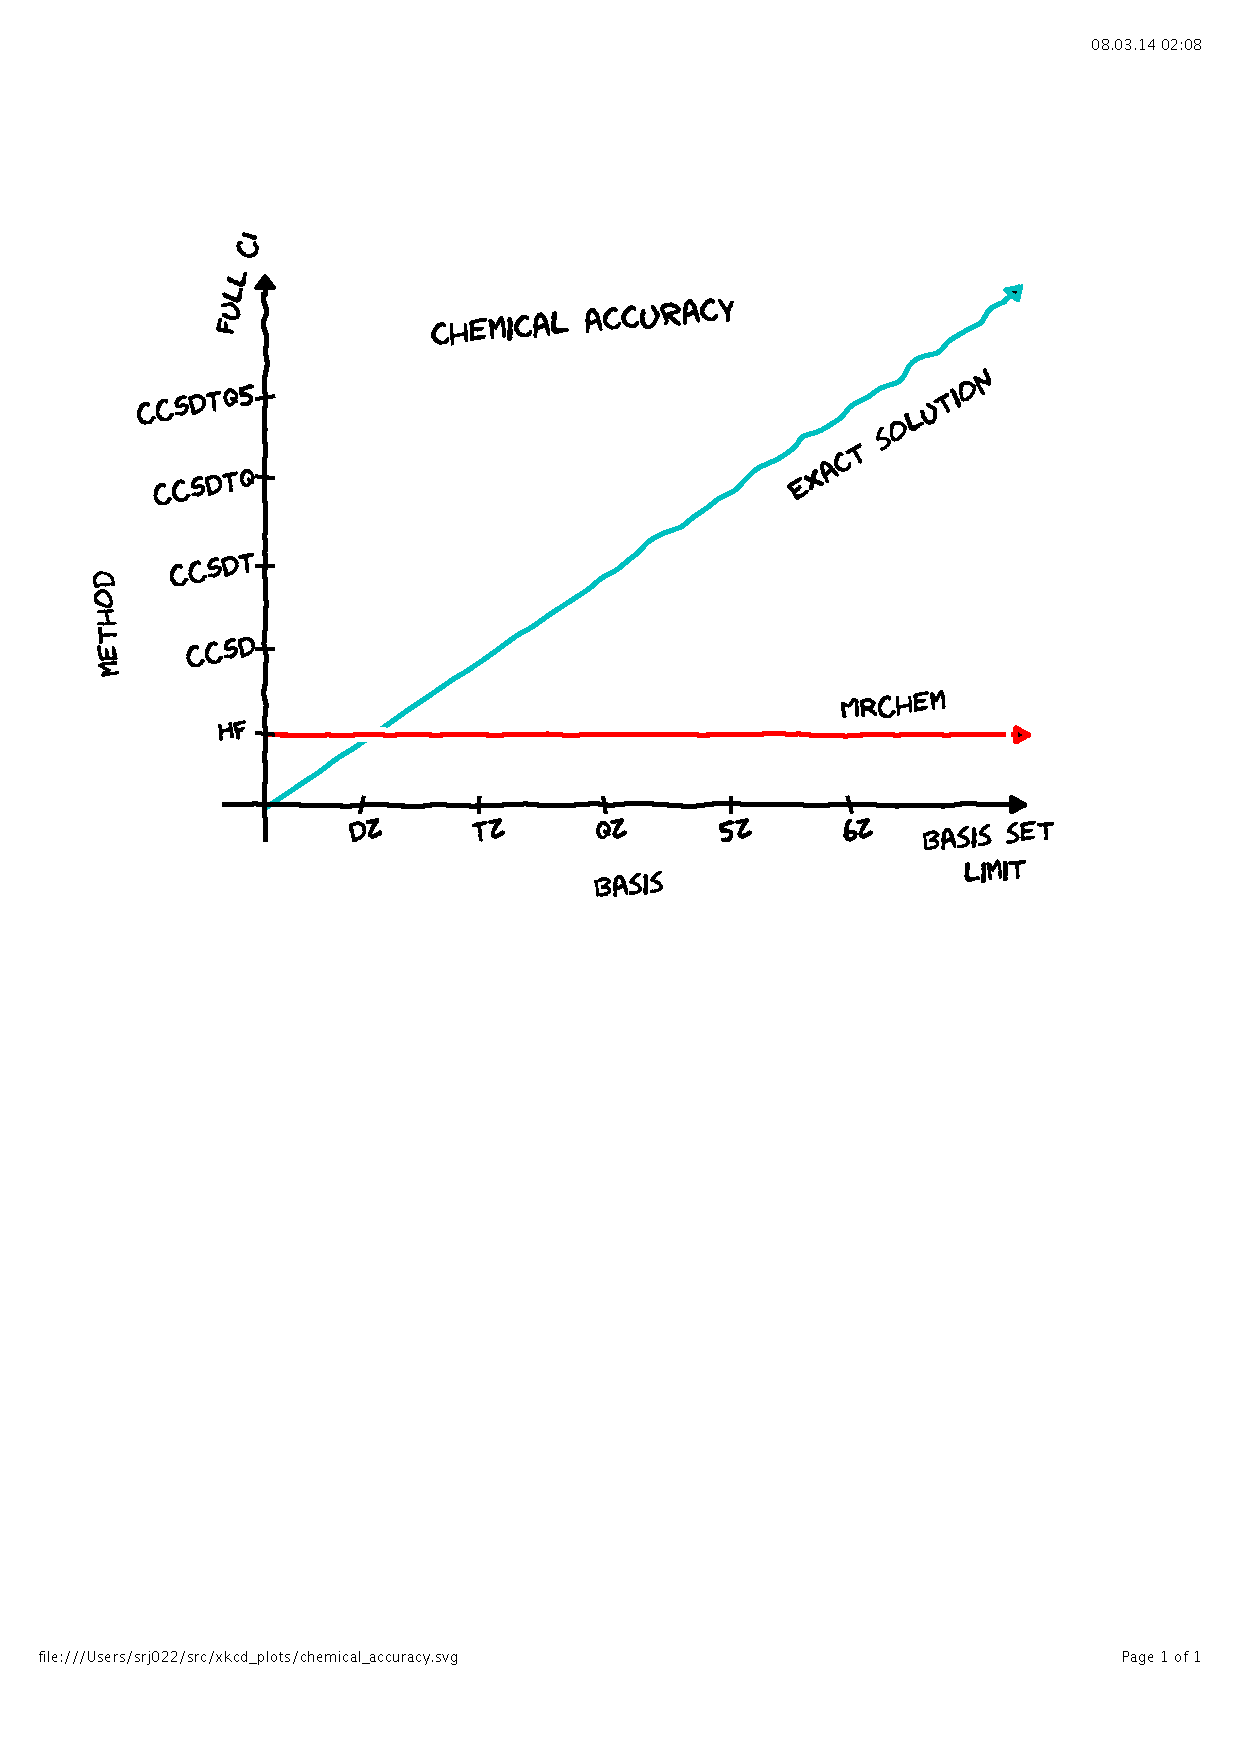
\includegraphics[scale=0.5, clip, viewport = 0 300 550 800]
        {figures/chemical_accuracy.pdf}}
    \end{center}
\end{frame}



\begin{frame}
    \centering
    \textbf{\Large{Multiwavelet Self-Consistent Field}}
\end{frame}

\begin{frame}
    \frametitle{Integral formulation SCF}
    \centering
    \textbf{Kohn-Sham equations}
    \begin{equation}
	\nonumber
	\bigg[-\frac{1}{2}\nabla^2 + \hat{V}\bigg]\orbital_i(r) = \epsilon_i \orbital_i(r)
    \end{equation}

    \vspace{5mm}

    \textbf{Rewrite using} $\mu_i^2 = -2\epsilon_i$
    \begin{align}
	\nonumber
	\Big[-\nabla^2 + \mu_i^2\Big]\orbital_i(r) =&\ -2\hat{V}\orbital_i(r)\\
	\nonumber
	\orbital_i(r) =&-2\Big[-\nabla^2 + \mu_i^2\Big]^{-1}\hat{V}\orbital_i(r)\\
	\nonumber
	\orbital_i =&-2\hat{G}_i\Big[\hat{V}\orbital_i\Big]
    \end{align}

    \vspace{5mm}

    \textbf{Bound-State Helmholtz operator}
    \begin{equation}
	\nonumber
	\hat{G}_if(r) = \int \frac{e^{-\mu_i |r-r'|}}{4\pi|r-r'|}f(r')dr'
    \end{equation}

    \vspace{5mm}

    \centering
    \tiny
    MH Kalos,
    {\it Phys. Rev.}, 
    \textbf{128(4)},
    1791 (1962)\\
    RJ Harrison, GI Fann, T Yanai, Z Gan and G Beylkin,
    {\it J. Chem. Phys.}, 
    \textbf{121},
    11587 (2004)
\end{frame}

\begin{frame}
    \frametitle{Hydrogen atom}
    \centering
    \textbf{Potential operator}
    \begin{equation}
	\nonumber
	\hat{V} = v_{nuc}(r) = -\sum_I\frac{Z_I}{|r-R_I|}
    \end{equation}

    \vspace{5mm}

    \textbf{Smoothed nuclear potential}
    \begin{align}
	\nonumber
	\frac{1}{r} &\approx \frac{erf(r)}{r} +
	\frac{1}{3\sqrt{\pi}}\big(e^{-r^2}+16e^{-4r^2}\big)
    \end{align}

    \vspace{5mm}

    \textbf{One-electron Schr\"{o}dinger equation}
    \begin{equation}
        \nonumber
        \Big[-\frac{1}{2}\nabla^2 + \hat{V}\Big]\psi(r) = E \psi(r)
    \end{equation}

    \vspace{1mm}

    \begin{equation}
        \nonumber
        \psi = -2\hat{G} \Big[\hat{V} \psi \Big]
    \end{equation}

    \vspace{5mm}

    \centering
    \tiny
    RJ Harrison, GI Fann, T Yanai, Z Gan and G Beylkin,
    {\it J. Chem. Phys.}, 
    \textbf{121},
    11587 (2004)
\end{frame}

\begin{frame}
    \frametitle{One-electron algorithm}
    \centering
    \textbf{Power iteration of the BSH operator}
    \begin{equation}
	\nonumber
	\psi^{n+1} = -2G^n\Big[\hat{V} \psi^n\Big]
    \end{equation}

    \vspace{3mm}

    \textbf{Finding roots of the residual}
    \begin{equation}
	\nonumber
	f(\psi) = -2G^n\big[\hat{V} \psi\big] -\psi
    \end{equation}

    \vspace{3mm}

    \textbf{Newton's method}
    \begin{equation}
	\nonumber
	\psi^{n+1} = \psi^n - \Big[J(\psi^n)\Big]^{-1} f(\psi^n)
    \end{equation}

    \begin{equation}
	\nonumber
	\psi^{n+1} = \psi^n - \Big[J(\psi^n)\Big]^{-1}
	\bigg(-2G^n\Big[\hat{V}\psi^n\Big] - \psi^n\bigg)
    \end{equation}

    \vspace{3mm}

    So the direct power iteration is an "inexact" Newton method\\
    where we approximate the Jacobian $J(\psi^n) \approx -1$.
\end{frame}

\begin{frame}
    \frametitle{One-electron algorithm}
    \begin{columns}
    \begin{column}{.50\textwidth}
    \centering
    \textbf{Initialize BSH operator} $\hat{G}^n$
    \begin{equation}
        \nonumber
        \mu^n = \sqrt{-2E^n}
    \end{equation}
    \end{column}

    \begin{column}{.50\textwidth}
    \centering
    \textbf{Power iteration}
    \begin{equation}
	\nonumber
	\tilde{\psi}^{n+1} = -2\hat{G}^n \Big[ \hat{V} \psi^n \Big]
    \end{equation}
    \end{column}
    \end{columns}

    \vspace{5mm}

    \begin{columns}
    \begin{column}{.50\textwidth}
    \centering
    \textbf{Wavefunction update}
    \begin{equation}
	\nonumber
	\Delta\psi^n = \frac{\tilde{\psi}^{n+1}}{\|\tilde{\psi}^{n+1}\|} - \psi^n
    \end{equation}
    \end{column}

    \begin{column}{.50\textwidth}
    \centering
    \textbf{Energy update}
    \begin{equation}
	\nonumber
	\Delta E^n =
        \frac{\langle\tilde{\psi}^{n+1}|\hat{V}|\Delta\tilde{\psi}^n\rangle}
        {\langle\tilde{\psi}^{n+1}|\tilde{\psi}^{n+1}\rangle}
    \end{equation}
    \end{column}
    \end{columns}

    \vspace{10mm}

    \centering
    \textbf{Update wavefunction and energy}
    \begin{align}
	\nonumber
        \psi^{n+1}  &= \psi^n + \Delta \psi^n\\
	\nonumber
        E^{n+1}     &= E^n + \Delta E^n
    \end{align}
\end{frame}

\begin{frame}
    \frametitle{One-electron algorithm}
    \centering
    \textbf{Using the relation}
    \begin{equation}
        \nonumber
        -2\hat{G}^n = \big(\hat{T} - E^n\big)^{-1}
    \end{equation}

    \vspace{5mm}

    \textbf{Manipulating the energy expression}
    \begin{align}
        \tilde{E}^{n+1}
        \nonumber
        &=	\langle\tilde{\psi}^{n+1}| \hat{T}+\hat{V} | \tilde{\psi}^{n+1}\rangle\\
        \nonumber
        &=	\langle\tilde{\psi}^{n+1}|  \hat{T} - E^n  | \tilde{\psi}^{n+1}\rangle
        +	\langle\tilde{\psi}^{n+1}|  E^n + \hat{V}  | \tilde{\psi}^{n+1}\rangle\\
        \nonumber
        &=	\langle\tilde{\psi}^{n+1}|  \hat{T} - E^n  | 
	        -2\hat{G}^n\big[\hat{V}\psi^n\big]\rangle
        +	\langle\tilde{\psi}^{n+1}| E^n + \hat{V} |\tilde{\psi}^{n+1}\rangle\\
        \nonumber
        &= -\langle\tilde{\psi}^{n+1}| \hat{V} |\psi^{n}\rangle
        +	\langle\tilde{\psi}^{n+1}| E^n + \hat{V} |\tilde{\psi}^{n+1}\rangle\\
        \nonumber
        &= E^{n}\langle\tilde{\psi}^{n+1}|\tilde{\psi}^{n+1}\rangle + 
	    \langle\tilde{\psi}^{n+1}| \hat{V} |\Delta\tilde{\psi}^{n}\rangle
    \end{align}

    \vspace{8mm}

    \centering
    \textbf{Energy without kinetic operator}
    \begin{equation}
        \nonumber
        E^{n+1} = E^{n} + 
        \frac{\langle\tilde{\psi}^{n+1}| \hat{V} |\Delta\tilde{\psi}^{n}\rangle}
        {\langle\tilde{\psi}^{n+1}|\tilde{\psi}^{n+1}\rangle}
    \end{equation}
\end{frame}

\begin{frame}
    \frametitle{Hydrogen atom}
    \only<1>{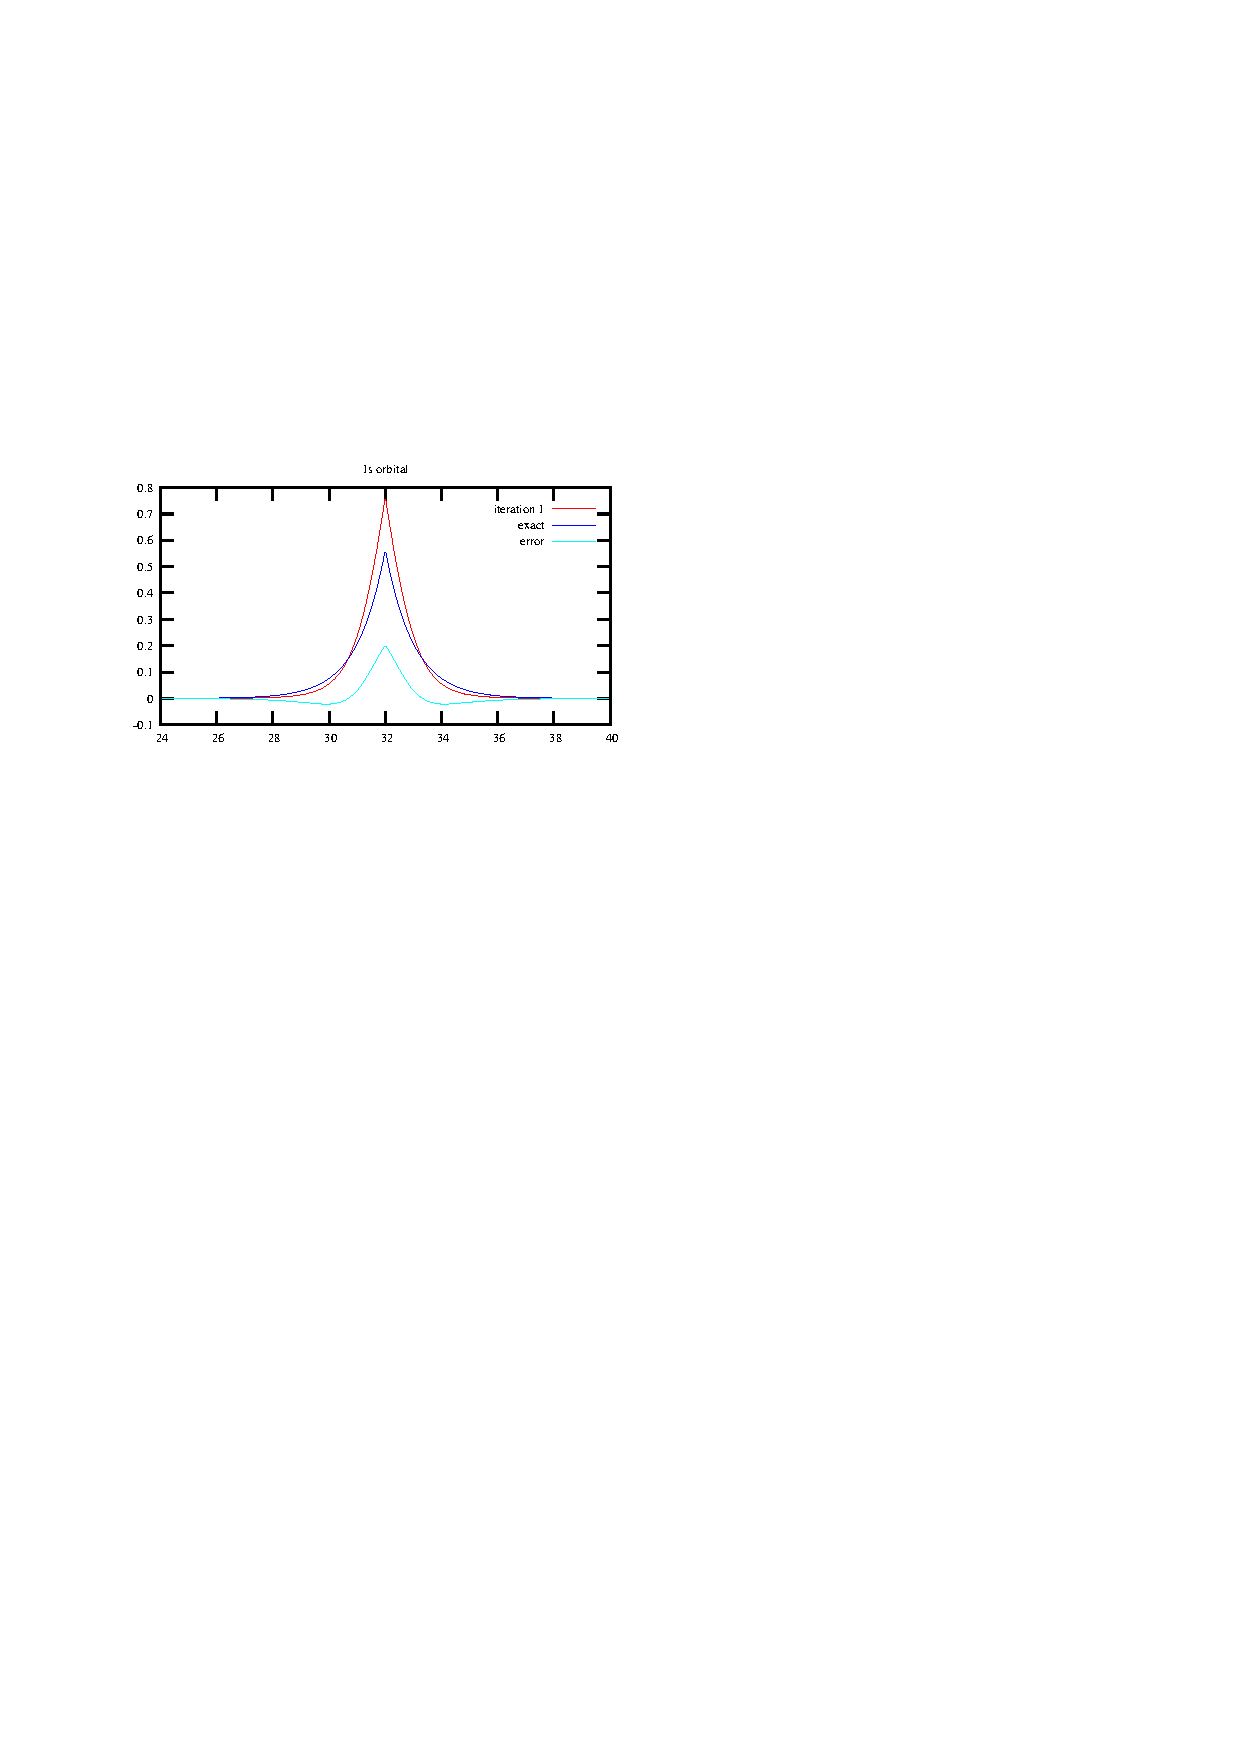
\includegraphics[viewport = 50 430 300 640, clip, scale=1.2]
       {figures/s1Orb_1.pdf}}
    \only<2>{\includegraphics[viewport = 50 430 300 640, clip, scale=1.2]
       {figures/s1Orb_2.pdf}}
    \only<3>{\includegraphics[viewport = 50 430 300 640, clip, scale=1.2]
       {figures/s1Orb_3.pdf}}
    \only<4>{\includegraphics[viewport = 50 430 300 640, clip, scale=1.2]
       {figures/s1Orb_4.pdf}}
    \only<5>{\includegraphics[viewport = 50 430 300 640, clip, scale=1.2]
       {figures/s1Orb_5.pdf}}
    \only<6>{\includegraphics[viewport = 50 430 300 640, clip, scale=1.2]
       {figures/s1Orb_10.pdf}}
\end{frame}

\begin{frame}
    \frametitle{Hydrogen atom}
    \begin{center}
	\includegraphics[scale=1.0, clip, viewport = 50 550 300 730]{figures/h_convergence.pdf}
    \end{center}
\end{frame}


\begin{frame}
    \frametitle{Krylov subspace Accelerated Inexact Newton (KAIN)}
    \begin{columns}
    \begin{column}[b]{0.5\textwidth}
    \centering
    \textbf{Wavefunction history}
    \begin{equation}
	\nonumber
	\psi^0, \psi^1, \dots, \psi^n
    \end{equation}
    \end{column}
    \begin{column}[b]{0.5\textwidth}
    \centering
    \textbf{Residual history}
    \begin{equation}
	\nonumber
	f(\psi^0), f(\psi^1), \dots, f(\psi^n)
    \end{equation}
    \end{column}
    \end{columns}

    \vspace{5mm}

    \centering
    \textbf{Used to find a better approximation to the Jacobian}

    \vspace{10mm}

    The new iterative step is then expanded in the Krylov subspace
    \begin{equation}
	\nonumber
	\delta\psi^n = \sum_i c_i\Big(\psi^i-\psi^n\Big) - 
	\sum_i c_i\Big(f(\psi^i) - f(\psi^n)\Big) - f(\psi^n)
    \end{equation}

    \vspace{5mm}

    by solving the linear system $Ac = b$
    \begin{align}
	\nonumber
	A_{ij} &= \langle\psi^n-\psi^i|f(\psi^n) - f(\psi^j)\rangle\\
	\nonumber
	b_{i}  &= \langle\psi^n-\psi^i|f(\psi^n)\rangle
    \end{align}

    \vspace{5mm}

    \centering
    \tiny
    RJ Harrison,
    {\it J. Comput. Chem.}, 
    \textbf{25(3)},
    328 (2004)
\end{frame}

\begin{frame}
    \frametitle{One-electron algorithm}

    \begin{columns}
    \begin{column}{.50\textwidth}
    \centering
    \textbf{Initialize BSH operator} $\hat{G}^n$
    \begin{equation}
        \nonumber
        \mu^n = \sqrt{-2E^n}
    \end{equation}
    \end{column}

    \begin{column}{.50\textwidth}
    \centering
    \textbf{Power iteration}
    \begin{equation}
	\nonumber
	\tilde{\psi}^{n+1} = -2\hat{G}^n \Big[ \hat{V} \psi^n \Big]
    \end{equation}
    \end{column}
    \end{columns}

    \vspace{5mm}

    \begin{columns}
    \begin{column}{.50\textwidth}
    \centering
    \textbf{Wavefunction update}
    \begin{equation}
	\nonumber
	\Delta\psi^n = \frac{\tilde{\psi}^{n+1}}{\|\tilde{\psi}^{n+1}\|} - \psi^n
    \end{equation}
    \end{column}

    \begin{column}{.50\textwidth}
    \centering
    \textbf{Energy update}
    \begin{equation}
	\nonumber
	\Delta E^n =
        \frac{\langle\tilde{\psi}^{n+1}|\hat{V}|\Delta\tilde{\psi}^n\rangle}
        {\langle\tilde{\psi}^{n+1}|\tilde{\psi}^{n+1}\rangle}
    \end{equation}
    \end{column}
    \end{columns}

    \vspace{5mm}

    \centering
    \textbf{KAIN update}
    \begin{equation}
	\nonumber
        \left(
        \begin{matrix}
        \delta \psi\\
        \delta E
        \end{matrix}
        \right)^{n+1}
        \longleftarrow
        \left(
        \begin{matrix}
        \psi\\
        E
        \end{matrix}
        \right)^n
        ,
        \left(
        \begin{matrix}
        \Delta \psi\\
        \Delta E
        \end{matrix}
        \right)^n
    \end{equation}

    \vspace{5mm}

    \textbf{Update wavefunction and energy}
    \begin{align}
	\nonumber
        \psi^{n+1}  &= \psi^n + \delta \psi^n\\
	\nonumber
        E^{n+1}     &= E^n + \delta E^n
    \end{align}
\end{frame}

\begin{frame}
    \frametitle{Hydrogen atom}
    \begin{center}
	\includegraphics[scale=1.0, clip, viewport = 300 550 560 740]{figures/h_convergence.pdf}
    \end{center}
\end{frame}

\begin{frame}
    \frametitle{Many-electron systems}
    \centering
    \textbf{Potential operator} $0 \leq \alpha \leq 1$
    \begin{equation}
        \nonumber
        \hat{V} = v_{nuc}(r) + v_{el}(r) + v_{xc}(r) - \alpha\hat{K}
    \end{equation}

    \vspace{10mm}

    \begin{columns}
    \begin{column}[b]{0.5\textwidth}
    \centering
    \textbf{Classical nuclear}
    \begin{equation}
        \nonumber
	v_{nuc}(r) = -\sum_I\frac{Z_I}{|r-R_I|}
    \end{equation}
    \end{column}

    \begin{column}[b]{0.5\textwidth}
    \centering
    \textbf{Classical Coulomb}
    \begin{equation}
        \nonumber
        v_{el}(r) = \int \frac{\rho(r')}{4\pi|r-r'|} \ud r'
    \end{equation}
    \end{column}
    \end{columns}

    \vspace{5mm}

    \begin{columns}
    \begin{column}[b]{0.5\textwidth}
    \centering
    \textbf{Exchange-Correlation}
    \begin{equation}
        \nonumber
        v_{xc}(r)
        %= \frac{\delta E_{xc}}{\delta \rho}
        = \frac{\partial F_{xc}}{\partial \rho} - \nabla \cdot \frac{\partial F_{xc}}{\partial \nabla\rho}
    \end{equation}
    \end{column}

    \begin{column}[b]{0.5\textwidth}
    \centering
    \textbf{Hartree-Fock exchange}
    \begin{equation}
        \nonumber
        \hat{K}\phi_p(r) = \sum_i \phi_i(r) \int \frac{\phi_i^\dagger(r')\phi_p(r')}{4\pi|r-r'|} \ud r'
    \end{equation}
    \end{column}
    \end{columns}
\end{frame}

\begin{frame}
    \frametitle{Orthonormalization}
    \centering
    \textbf{Straightforward iteration of the Kohn-Sham equations}
    \begin{equation}
        \nonumber
        \tilde{\phi}_i^{n+1} = -2\hat{G}_i^n \bigg[\hat{V}^n\phi_i^n\bigg]
    \end{equation}
    \textbf{brings all orbitals to the lowest energy eigenfunction}
    
    \vspace{15mm}

    \textbf{Orthonormality must be imposed}
    \begin{equation}
        \nonumber
        \tilde{S}_{ij} = \langle\tilde{\phi}_i|\tilde{\phi}_j\rangle = \delta_{ij}
    \end{equation}

    \vspace{5mm}

    \begin{columns}
    \begin{column}[b]{0.5\linewidth}
    \centering
    \textbf{Gram-Schmidt}
    \begin{equation}
	\nonumber
	\phi_i = \Big(1 - \sum_{j<i}|\phi_j\rangle\langle\phi_j|\Big)\tilde{\phi}_i
    \end{equation}
    \end{column}

    \begin{column}[b]{0.5\linewidth}
    \centering
    \textbf{L\"{o}wdin orthonormalization}
    \begin{equation}
	\nonumber
	\phi_i = \sum_j \tilde{S}_{ij}^{-1/2}\tilde{\phi}_j
    \end{equation}
    \end{column}
    \end{columns}
\end{frame}

\begin{frame}
    \frametitle{Non-canonical orbitals}
    \centering
    \textbf{The non-canonical Kohn-Sham equations}
    \begin{equation}
        \nonumber
        \hat{F}|\phi_i\rangle 
        = \bigg[\sum_j|\phi_j\rangle\langle\phi_j|\bigg]\hat{F}|\phi_i\rangle
        = \sum_jF_{ji}|\phi_j\rangle
    \end{equation}

    \vspace{5mm}

    \textbf{Rewrite using} $\mu_i^2 = -2\lambda_i$
    \begin{align}
        \nonumber
        \bigg[-\frac{1}{2}\nabla^2 + \hat{V}\bigg]\phi_i
        &= \sum_jF_{ji}\phi_j\\
        \nonumber
        \bigg[-\nabla^2 + \mu_i^2\bigg]\phi_i 
        &= -2\bigg[\hat{V}\phi_i - \sum_j\big(F_{ji} -
        \lambda_i\delta_{ji}\big)\phi_j\bigg]\\
        \nonumber
        \phi_i
        &= -2\hat{G}_i\bigg[\hat{V}\phi_i - \sum_j\big(F_{ji} -
        \Lambda_{ji}\big)\phi_j\bigg]
    \end{align}

    \vspace{5mm}

    \begin{columns}
    \begin{column}[b]{0.48\linewidth}
    \centering
    \textbf{Fock matrix}
    \begin{equation}
        \nonumber
        F_{ij} = \langle\phi_i|\hat{T} + \hat{V}|\phi_j\rangle
    \end{equation}
    \end{column}

    \begin{column}[b]{0.48\linewidth}
    \centering
    \textbf{Kinetic matrix}
    \begin{equation}
        \nonumber
        T_{ij}
        = \langle\phi_i|\hat{T}|\phi_j\rangle
        = \frac{1}{2}\langle\nabla\phi_i|\nabla\phi_j\rangle
    \end{equation}
    \end{column}
    \end{columns}
\end{frame}

\begin{frame}
    \frametitle{Localized orbitals}
    \centering
    Total energy invariant under unitary transformations among occupied orbitals
    \begin{equation}
	\nonumber
	\phi_i = \sum_j L_{ij} \phi_i, \qquad \qquad L^\ast L = LL^\ast = I
    \end{equation}

    \begin{columns}
    \begin{column}[b]{0.48\linewidth}
    \centering
    \includegraphics[scale=0.25, clip, viewport = 80 560 600 700]{figures/alkane.pdf}\\
    \includegraphics[scale=0.25, clip, viewport = 80 560 600 700]{figures/can_orb_1.pdf}\\
    \includegraphics[scale=0.25, clip, viewport = 80 560 600 700]{figures/can_orb_2.pdf}\\

    \vspace{2mm}

    \begin{equation}
        \nonumber
        \phi_i =\ -2\hat{G}_i\Bigg[\hat{V}\phi_i
        - (\epsilon_i - \lambda_i)\phi_i\Bigg]
    \end{equation}
    \end{column}

    \begin{column}[b]{0.48\linewidth}
\only<2>{
    \centering
    \includegraphics[scale=0.25, clip, viewport = 80 560 600 700]{figures/loc_orb_1.pdf}\\
    \includegraphics[scale=0.25, clip, viewport = 80 560 600 700]{figures/loc_orb_2.pdf}\\
    \includegraphics[scale=0.25, clip, viewport = 80 560 600 700]{figures/loc_orb_3.pdf}\\

    \vspace{2mm}

    \begin{equation}
        \nonumber
        \phi_i =\ -2\hat{G}_i\Bigg[\hat{V}\phi_i
        - \sum_j(F_{ji} - \Lambda_{ji})\phi_j\Bigg]
    \end{equation}
}
    \end{column}
    \end{columns}

    \vspace{6mm}

    \centering
    \tiny
    S.F. Boys,
    {\it Rev. Mod. Phys.}, 
    \textbf{32:296}
    (1960)\\
    J.M. Foster, S.F. Boys,
    {\it Rev. Mod. Phys.}, 
    \textbf{32:300}
    (1960)
\end{frame}

\begin{frame}
    \frametitle{Many-electron algorithm I}
    \centering
    \textbf{Setup Fock operator} $\hat{F}^n$

    \vspace{5mm}

    \textbf{Compute Fock matrix} $F_{ij}^n = \langle\phi_i^n|\hat{F}^n|\phi_j^n\rangle$

    \vspace{5mm}

    \textbf{Diagonalize/Localize}

    \vspace{5mm}

    \textbf{Iterate BSH operators with} $\lambda_i^n \approx F_{ii}^n$
    \begin{equation}
	\nonumber
        \tilde{\phi}_i^{n+1} = -2\hat{G}_i^n \bigg[\hat{V}^n\phi_i^n -
        \sum_j\big(F_{ji}^n - \Lambda_{ji}^n\big)\phi_j^n\bigg]
    \end{equation}

    \vspace{2mm}

    \textbf{Orthonormalize} $S^{-1/2}$

    \vspace{5mm}

    \textbf{Compute KAIN update} $\delta\phi_i^n$

    \vspace{5mm}

    \textbf{Orthonormalize} $S^{-1/2}$

\end{frame}

\begin{frame}
    \frametitle{Many-electron algorithm I}
    \centering
    \textbf{Overall accuracy kept at} $\epsilon = 10^{-6}$
    \begin{center}
	\includegraphics[scale=1.0, clip, viewport = 50 550 300 740]{figures/accuracy.pdf}
    \end{center}
\end{frame}

\begin{frame}
    \frametitle{Many-electron algorithm I}
    \begin{columns}
    \begin{column}[b]{0.70\linewidth}
        \centering
        \includegraphics[scale=0.8, clip, viewport = 50 550 300 730]{figures/benzene_convergence.pdf}
    \end{column}
    \begin{column}[b]{0.30\linewidth}
        \centering
        \textbf{Benzene}
        \includegraphics[scale=0.1, clip, viewport = 0 0 1000 1200]{figures/benzene.png}

        \vspace{5mm}

    \end{column}
    \end{columns}
\end{frame}

\begin{frame}
    \frametitle{Fock matrix update}
    \centering
    \textbf{Using the relation}
    \begin{equation}
        \nonumber
        -2\hat{G}_i^n = \big(\hat{T} - \lambda_i^n\big)^{-1}
    \end{equation}

    \vspace{3mm}

    \textbf{Manipulating the Fock matrix expression}
    \begin{align}
        \nonumber
        \tilde{F}_{ij}^{n+1}    &= 
        \langle\tilde{\phi}_i^{n+1} |
        \hat{T} + \hat{V}^{n+1}     |
        \tilde{\phi}_j^{n+1}\rangle\\
        \nonumber
			    &= 
        \langle\tilde{\phi}_i^{n+1} |
        \hat{T} - \lambda_j^n       |
        \tilde{\phi}_j^{n+1}\rangle +
        \langle\tilde{\phi}_i^{n+1} |
        \hat{V}^{n+1} + \lambda_j^n |
        \tilde{\phi}_j^{n+1}\rangle\\
        \nonumber
        &\ \ \vdots
    \end{align}

    \textbf{Potential updates}
    \begin{equation}
        \nonumber
        \big(\Delta\tilde{F}_{pot}^n\big)_{ij} =
        \langle\tilde{\phi}_i^{n+1} |
        \hat{V}^n                       |
        \Delta\tilde{\phi}_j^n\rangle + 
        \langle\tilde{\phi}_i^{n+1} |
        \Delta\hat{V}^n                 |
        \phi_j^n\rangle
    \end{equation}

    \vspace{3mm}

    \textbf{Overlap updates}
    \begin{equation}
    \nonumber
        \big(\Delta\tilde{S}_1^n\big)_{ij} =
        \langle\Delta\tilde{\phi}_i^n | \phi_j^n\rangle \qquad \qquad
        \big(\Delta \tilde{S}_2^n\big)_{ij} =
        \langle\tilde{\phi}_i^{n+1} | \Delta\tilde{\phi}_j^n\rangle
    \end{equation}

    \vspace{3mm}

    \centering
    \textbf{Fock matrix without kinetic operator}
    \begin{equation}
        \nonumber
        \tilde{F}^{n+1} = F^{n} + 
        \Delta \tilde{S}_1^n F^n +
        \Delta \tilde{S}_2^n \Lambda^n +
        \Delta \tilde{F}_{pot}^n
    \end{equation}
\end{frame}

\begin{frame}
    \frametitle{Many-electron algorithm II}
    \centering
    \textbf{Setup Fock operator} $\hat{F}^n$

    \vspace{8mm}

    \textbf{Iterate BSH operators with} $\lambda_i^n \approx F_{ii}^n$
    \begin{equation}
	\nonumber
        \tilde{\phi}_i^{n+1} = -2\hat{G}_i^n \bigg[\hat{V}^n\phi_i^n -
        \sum_j\big(F_{ji}^n - \Lambda_{ji}^n\big)\phi_j^n\bigg]
    \end{equation}

    \vspace{2mm}

    \textbf{Compute potential updates} $\Delta\hat{V}^n$

    \vspace{8mm}

    \textbf{Update Fock matrix}
    \begin{equation}
        \nonumber
        \tilde{F}^{n+1} = F^{n} + 
        \Delta \tilde{S}_1^n F^n +
        \Delta \tilde{S}_2^n \Lambda^n +
        \Delta \tilde{F}_{pot}^n
    \end{equation}

    \vspace{5mm}

    \textbf{Orthonormalize} $\tilde{S}^{-1/2}$

    \vspace{5mm}

    \textbf{Diagonalize/localize}

\end{frame}

\begin{frame}
\frametitle{Ground state energy}
\scriptsize
\centering
\begin{table}
    \centering
    \begin{tabular}{lr@{.}lr@{.}l}
    \multicolumn{5}{c}{\textbf{LDA energy of Argon (a.u.)}}\\
    \hline
    \hline
                        &\multicolumn{4}{c}{}   \\
    &\multicolumn{2}{c}{HOMO}
    &\multicolumn{2}{c}{Total}\\
                        &\multicolumn{4}{c}{}   \\
    MW $\epsilon=10^{-3}$  &-0&38\red{7692}&-525&966\red{790}  \\
    MW $\epsilon=10^{-5}$  &-0&3823\red{48}&-525&9461\red{09}  \\
    MW $\epsilon=10^{-7}$  &-0&382330      &-525&94619\red{6}  \\
                           &\multicolumn{4}{c}{}   \\
    NIST                   &-0&382330      &-525&946195  \\
                           &\multicolumn{4}{c}{}   \\
    aug-cc-pV6Z		   &-0&3823\red{23}&-525&94\red{4181}  \\
    %aug-cc-pV5Z		   &-0&3823\red{88}&-525&94\red{2021}  \\
    aug-cc-pVQZ		   &-0&382\red{463}&-525&93\red{8021}  \\
    %aug-cc-pVTZ	           &-0&382\red{838}&-525&9\red{33682}  \\
    aug-cc-pVDZ		   &-0&382\red{143}&-525&9\red{15702}  \\
                           &\multicolumn{4}{c}{}   \\
    \hline
    \hline
    \end{tabular}
\end{table}

\vspace{1mm}

\tiny

\it{NIST: National Institute of Standards and Technology (Basis set limit)}\\
\it{GTO calculations using Dalton}

\vspace{5mm}

\scriptsize

\begin{itemize}
    \item   We are able to attain \textbf{considerably higher} accuracy than 
            high-quality GTOs
    \item   Energies are not variational, but \textbf{basis set limit} within 
            the requested precision
\end{itemize}

\end{frame}

\begin{frame}
\frametitle{Ground state energy}
\scriptsize

\centering
\textbf{Methyloxirane molecule}
\hspace{30mm}
\textbf{Adaptive grid}
\begin{minipage}{0.5\textwidth}
\centering
\includegraphics[scale=0.15, viewport = 0 180 550 650, clip]{figures/methyloxirane_white.jpg}
\end{minipage}%
\begin{minipage}{0.5\textwidth}
\centering
\includegraphics[angle=-90, scale=0.25, viewport = 170 150 470 700, clip]{figures/methyloxirane_grid.pdf}
\end{minipage}
\begin{table}
    \centering
    \textbf{Total wall time on 16 CPUs}
    \begin{tabular}{rcr|rcr}
    \hline               
    \hline               
                         &                    &                &                  &                   &                  \\
    MRChem               & PBE energy (a.u.)  & Time           & Dalton           & PBE energy (a.u.) & Time             \\
    \hspace{10mm}\       & \hspace{20mm}\     & \hspace{05mm}\ & \hspace{10mm}\   & \hspace{05mm}\    & \hspace{05mm}\   \\
    $\epsilon = 10^{-2}$ & -191.\red{??????}  &  ??m           & aug-cc-pVDZ      & -191.\red{??????} &  ??m             \\
    $\epsilon = 10^{-3}$ & -191.?\red{?????}  &  ??m           & aug-cc-pVTZ      & -191.?\red{?????} &  ??m             \\
    $\epsilon = 10^{-4}$ & -191.??\red{????}  &  ??m           & aug-cc-pVQZ      & -191.??\red{????} &  ??m             \\
    $\epsilon = 10^{-5}$ & -191.???\red{???}  &  ??m           & aug-cc-pV5Z      & -191.???\red{???} &  ??m             \\
    $\epsilon = 10^{-6}$ & -191.????\red{??}  &  ??m           & aug-cc-pV6Z      & -191.????\red{??} &  ??m             \\
                         &                    &                \\
    \hline
    \hline
    \end{tabular}
\end{table}
\end{frame}

\begin{frame}
    \frametitle{Ground state energy}
    scaling plot MRChem vs Dalton
\end{frame}



%\begin{frame}
    \frametitle{Integral formulation linear response}
    \centering
    The Sternheimer equations (coupled-perturbed HF/KS)
    \begin{equation}
        \nonumber
        \hat{F}^{(0)}\ket{\orbital_i^{(1)}} + \hat{F}^{(1)}\ket{\orbital_i^{(0)}} = 
        \sum_jF_{ij}^{(0)}\ket{\orbital_j^{(1)}} + \sum_j F_{ij}^{(1)}\ket{\orbital_j^{(0)}}
    \end{equation}

    \vspace{10mm}

    are solved in the same way as the ground state
    \begin{equation}
        \nonumber
        \ket{\orbital_i^{(1)}} =\
        -2\Helmholtz{\hat{V}^{(0)}\ket{\orbital_i^{(1)}}
        + \left(1 - \hat{\rho}^{(0)}\right)\hat{F}^{(1)}\ket{\orbital_i^{(0)}}}
    \end{equation}

%\vspace{5mm}
%\centering
%\tiny
%T. Yanai \etal,
%{\it Mol. Phys.},
%\textbf{103:2-3} 
%(2005)\\
%H. Sekino \etal,
%{\it J. Chem. Phys.},
%\textbf{129} 
%(2008)\\
%T. Yanai, \etal,
%\it{Phys. Chem. Chem. Phys.}, 
%\textbf{17}
%(2015)

\end{frame}

%\begin{frame}
%\frametitle{Integral formulation linear response}
%
%\begin{columns}
%\begin{column}[b]{0.48\linewidth}
%\centering
%\textbf{Time-dependent perturbation}
%\begin{align}
%    \nonumber
%    \hat{H}^{(1)}(t) &= 
%    \hat{h}^{(1)}e^{i\omega t} +
%    \hat{h}^{(1)\dag}e^{-i\omega t}\\
%    \nonumber
%    &\ \\
%    \nonumber
%    \rho^{(1)}(t) &= 
%    \tilde{\rho}^{(1)}e^{i\omega t} +
%    \tilde{\rho}^{(1)\dag}e^{-i\omega t}\\
%    \nonumber
%    &\ \\
%    \nonumber
%    \pert{\tilde{\rho}}{1}(r,r') &= 
%    \sum_i x_i(r)\orbital_i^\dag(r') + \orbital_i(r)y_i^\dag(r')
%\end{align}
%\end{column}
%
%\begin{column}[b]{0.48\linewidth}
%\centering
%\textbf{First-order operators}
%\begin{align}
%    \nonumber
%    \pert{\coulomb}{1} \orbital_p &=
%        \int\frac{\pert{\tilde{\rho}}{1}(r',r')\orbital_p(r)}{|r-r'|} \ud r' \\
%    \nonumber
%    \pert{\exchange}{1} \orbital_p &=
%        \int\frac{\pert{\tilde{\rho}}{1}(r,r')\orbital_p(r')}{|r-r'|} \ud r' \\
%    \nonumber
%    \pert{\xc}{1} \orbital_p &= 
%        \bigg[\frac{\delta^2 E_{xc}}{\delta \rho^2}
%        \big[\pert{\rho}{0}\big]*\pert{\tilde{\rho}}{1}\bigg] \orbital_p
%\end{align}
%\end{column}
%\end{columns}
%
%\vspace{7mm}
%\centering
%\textbf{Working equations for dynamic linear response}
%\begin{align}
%    \nonumber
%    x_i &= -2 \Helmholtzp{
%    \pert{\potential}{0}x_i +
%    \Big(1 - \pert{\density}{0}\Big)
%    \Big(\pert{\hamiltonian}{1} + \pert{\potential}{1}\Big)\orbital_i}\\
%    \nonumber
%    y_i &= -2 \Helmholtzm{
%    \pert{\potential}{0}y_i +
%    \Big(1 - \pert{\density}{0}\Big)
%    \Big(\pert{\hamiltonian}{1} + \pert{\potential}{1}\Big)^\dag\orbital_i}
%\end{align}
%
%
%\vspace{7mm}
%
%\begin{columns}
%\begin{column}[b]{0.48\linewidth}
%\centering
%\textbf{BSH operators} 
%\begin{equation}
%    \nonumber
%    2\hat{G}_i^{(\pm)} = \Big[\hat{T} - (\epsilon_i \pm \omega)\Big]^{-1} 
%\end{equation}
%\end{column}
%
%\begin{column}[b]{0.48\linewidth}
%\centering
%\textbf{Density operator}
%\begin{equation}
%    \nonumber
%    \pert{\density}{0} = \sum_i \ket{\orbital_i}\bra{\orbital_i}
%\end{equation}
%\end{column}
%\end{columns}
%
%\vspace{5mm}
%\centering
%\tiny
%T. Yanai \etal,
%{\it Mol. Phys.},
%\textbf{103:2-3} 
%(2005)\\
%H. Sekino \etal,
%{\it J. Chem. Phys.},
%\textbf{129} 
%(2008)\\
%T. Yanai, \etal,
%\it{Phys. Chem. Chem. Phys.}, 
%\textbf{(published online)},
%(2015)
%
%\end{frame}

%\begin{frame}
%\frametitle{Polarizability}
%\begin{columns}
%
%\begin{column}[b]{0.3\textwidth}
%\centering
%\textbf{Electric dipole operator}
%\begin{equation}
%    \nonumber
%    \pert{\hamiltonian}{E} = \boldsymbol{r}_O
%\end{equation}
%\end{column}
%
%
%\begin{column}[b]{0.7\textwidth}
%\centering
%\textbf{Polarizability}
%\begin{equation}
%    \nonumber
%    \alpha 
%    %= \int \pert{\hamiltonian}{E} \ \pert{\rho}{E} \ dr
%    = \sum_i 
%    \bra{\orbital_i}\pert{\hamiltonian}{E} \ket{\pert{x_i}{E}} + 
%    \bra{\pert{y_i}{E}}\pert{\hamiltonian}{E}\ket{\orbital_i}
%\end{equation}
%\end{column}
%\end{columns}
%
%\vspace{5mm}
%
%
%\begin{table}
%%\tiny
%\begin{tabular}{r|c|cr|cr}
%\multicolumn{6}{c}{\textbf{LDA polarizability of methyloxirane (a.u.)}}\\
%\hline
%\hline
%	             &               &               &               &               &               \\
%                     & $E^{tot}$     & Static        &Time           & Dynamic       &Time           \\
%    \hspace{20mm}\   &\hspace{20mm}\ &\hspace{20mm}\ &\hspace{05mm}\ &\hspace{20mm}\ &\hspace{05mm}\ \\
%    MRChem $10^{-2}$ & -191.5975     & 44.0764       &   30m         & 45.2747       &   1h          \\
%    MRChem $10^{-3}$ & -191.5622     & 44.0939       &    1h         & 45.2907       &   2h          \\
%    MRChem $10^{-4}$ & -191.5619     & 44.0935       &    2h         & 45.2903       &   3h          \\
%	             &               &               &               &               &               \\
%    aug-cc-pVQZ      & -191.5563     & 44.1326       &    1h         & 45.3380       &   2h          \\
%	cc-pVQZ      & -191.5549     & 42.3602       &   30m         & 43.4064       &   1h          \\
%    aug-cc-pVDZ      & -191.4817     & 44.0050       &    1m         & 45.2025       &   2m          \\
%	cc-pVDZ      & -191.4622     & 36.5586       &    $<$1m      & 37.3993       &   1m          \\
%	             &               &               &               &               &               \\
%\hline
%\hline
%\end{tabular}
%\end{table}
%
%\centering
%\it{Wall time given on 16 CPUs}\\
%\it{GTO calculations using Dalton}\\
%\it{Dynamic response at sodium D line (589.3 nm) wavelength}
%
%\end{frame}


%\begin{frame}
%\frametitle{Magnetizability}
%\begin{columns}
%
%\begin{column}[b]{0.5\textwidth}
%\centering
%\textbf{Diamagnetic magnetizability}
%\begin{equation}
%    \nonumber
%    \pert{\hamiltonian}{B,B} = 
%    -\frac{1}{4}\Big(r_O^2\boldsymbol{I} 
%    -\boldsymbol{r}_O\boldsymbol{r}_O^T\Big)
%\end{equation}
%
%\vspace{2mm}
%
%\begin{align}
%    \nonumber
%    \chi^{dia} &= \sum_i \bra{\orbital_i} \pert{\hamiltonian}{B,B} \ket{\orbital_i}
%%    \nonumber
%%    \chi^{dia} &= \int \pert{\hat{h}}{dia} \rho \ud r
%\end{align}
%\end{column}
%
%\begin{column}[b]{0.5\textwidth}
%\centering
%\textbf{Paramagnetic magnetizability}
%\begin{equation}
%    \nonumber
%    \pert{\hamiltonian}{B} = -i \boldsymbol{r}_O\times\nabla
%\end{equation}
%\vspace{2mm}
%\begin{align}
%    \nonumber
%    \chi^{para} &= \sum_i 
%    \bra{\orbital_i}\pert{\hamiltonian}{B} \ket{\pert{x_i}{B}} + 
%    \bra{\pert{y_i}{B}}\pert{\hamiltonian}{B}\ket{\orbital_i}
%%    \nonumber
%%    \chi^{para} &= \int \pert{\hat{h}}{orb}\pert{\tilde{\rho}}{orb} \ud r
%\end{align}
%\end{column}
%
%\end{columns}
%\vspace{6mm}
%
%\begin{table}
%%\tiny
%\centering
%\begin{tabular}{r|c|crrr}
%\multicolumn{6}{c}{\textbf{Hartree-Fock magnetizability of methyloxirane (a.u.)}}\\
%\hline
%\hline
%                     &               &               &                     &                     &               \\
%                     &$E^{tot}$      & GIAO          & $O=(0,0,0)$         & $O=(5,5,5)$         &Time           \\
%    \hspace{15mm}\   &\hspace{15mm}\ &\hspace{15mm}\ &\hspace{15mm}\       &\hspace{15mm}\       &\hspace{05mm}\ \\
%    MRChem $10^{-2}$ & -192.0425     &               &  -9.5497\ \ \ \ \ \ &  -9.9222\ \ \ \ \ \ &    4h         \\
%    MRChem $10^{-3}$ & -192.0002     &               &  -9.4730\ \ \ \ \ \ &  -9.4363\ \ \ \ \ \ &    6h         \\
%    MRChem $10^{-4}$ & -192.0000     &               &  -9.4758\ \ \ \ \ \ &  -9.4795\ \ \ \ \ \ &   12h         \\
%                     &               &               &                     &                     &               \\
%    aug-cc-pVQZ      & -191.9968     & -9.4736       & -10.5253\ \ \ \ \ \ & -26.0533\ \ \ \ \ \ &    2h         \\
%	cc-pVQZ      & -191.9960     & -9.4681       & -10.8019\ \ \ \ \ \ & -29.2395\ \ \ \ \ \ &    1h         \\
%    aug-cc-pVDZ      & -191.9357     & -9.5369       & -15.4438\ \ \ \ \ \ &-101.6430\ \ \ \ \ \ &    1m         \\
%	cc-pVDZ      & -191.9232     & -9.4924       & -19.0342\ \ \ \ \ \ &-140.0203\ \ \ \ \ \ &    $<$1m      \\
%                     &               &               &                     &                     &               \\
%\hline
%\hline
%\end{tabular}
%\end{table}
%
%\centering
%\it{Wall time given on 16 CPUs}\\
%\it{GTO calculations using Dalton}
%
%\end{frame}


%\begin{frame}
%\frametitle{Nuclear shielding}
%\begin{columns}
%
%\begin{column}[b]{0.4\textwidth}
%\centering
%\textbf{Diamagnetic shielding}
%\begin{equation}
%    \nonumber
%    \pert{\hamiltonian}{M_K,B} =
%    \frac{\alpha}{2}\frac{\Big(r_O^Tr_K\boldsymbol{I} - 
%    \boldsymbol{r}_O\boldsymbol{r}_O^T\Big)}{r_K^3}
%\end{equation}
%\vspace{2mm}
%\begin{equation}
%    \nonumber
%    \xi^{dia} = \sum_i \bra{\orbital_i} \pert{\hamiltonian}{M_K,B} \ket{\orbital_i}
%\end{equation}
%\end{column}
%
%\begin{column}[b]{0.6\textwidth}
%\centering
%\textbf{Paramagnetic shielding}
%\begin{equation}
%    \nonumber
%    \pert{\hamiltonian}{M_K} 
%    = -i \alpha^2 \frac{\boldsymbol{r}_K\times\nabla}{r_K^3} \qquad \qquad
%    \pert{\hamiltonian}{B} = -i \boldsymbol{r}_O\times\nabla
%\end{equation}
%\vspace{2mm}
%\begin{equation}
%    \nonumber
%    \xi^{para} = \sum_i 
%    \bra{\orbital_i}\pert{\hamiltonian}{M_K} \ket{\pert{x_i}{B}} + 
%    \bra{\pert{y_i}{B}}\pert{\hamiltonian}{M_K}\ket{\orbital_i}
%\end{equation}
%\end{column}
%
%\end{columns}
%\vspace{5mm}
%
%\begin{table}
%%\tiny
%\centering
%\begin{tabular}{r|c|cccr}
%\multicolumn{6}{c}{\textbf{Hartree-Fock shielding tensor of oxygen in methyloxirane (ppm)}}\\
%\hline
%\hline
%                     &               &               &               &               &               \\
%                     & $E^{tot}$     &$\xi^{dia}$    & $\xi^{para}$  &$\xi^{tot}$    &Time           \\
%       	             &\hspace{15mm}\ &\hspace{15mm}\ &\hspace{15mm}\ &\hspace{15mm}\ &\hspace{05mm}\ \\
%    MRChem $10^{-2}$ & -192.0425     &  446.7869     &  -96.6166     &  350.1703     &    4h         \\
%    MRChem $10^{-3}$ & -192.0002     &  447.3444     &  -91.7855     &  355.5589     &    6h         \\
%    MRChem $10^{-4}$ & -192.0000     &  447.3089     &  -90.9386     &  356.3704     &   12h         \\
%	             &               &               &               &               &               \\
%    aug-cc-pVQZ      & -191.9968     &  447.7508     &  -90.6691     &  357.0817     &    2h         \\
%	cc-pVQZ      & -191.9960     &  447.7833     &  -89.6304     &  358.1529     &    1h         \\
%    aug-cc-pVDZ      & -191.9357     &  451.0119     &  -88.5778     &  362.4341     &    1m         \\
%	cc-pVDZ      & -191.9232     &  451.6103     &  -87.4153     &  364.1950     &    $<$1m      \\
%	             &               &               &               &               &               \\
%\hline
%\hline
%\end{tabular}
%\end{table}
%
%\centering
%\it{Wall time given on 16 CPUs}\\
%\it{GTO (GIAOs) calculations using Dalton}
%
%\end{frame}
%
%
%\begin{frame}
%\frametitle{Optical rotation}
%\begin{columns}
%
%\begin{column}[b]{0.5\textwidth}
%\centering
%\textbf{Electric-magnetic polarizability}
%\begin{equation}
%    \nonumber
%    \pert{\hamiltonian}{E} = \boldsymbol{r}_O \qquad \qquad
%    \pert{\hamiltonian}{B} = -i \boldsymbol{r}_O\times\nabla
%\end{equation}
%\vspace{4mm}
%\begin{equation}
%    \nonumber
%    G = \sum_i 
%    \bra{\orbital_i}\pert{\hamiltonian}{B} \ket{\pert{x_i}{E}} + 
%    \bra{\pert{y_i}{E}}\pert{\hamiltonian}{B}\ket{\orbital_i}
%\end{equation}
%\end{column}
%
%\begin{column}[b]{0.5\textwidth}
%\centering
%\textbf{Optical rotation}
%\vspace{2mm}
%\begin{equation}
%    \nonumber
%    \beta = \omega^{-1}Tr\big[G\big]
%\end{equation}
%\vspace{2mm}
%\begin{equation}
%    \nonumber
%    \alpha = \frac{28800\pi^2N_A\nu^2}{c^2M}\beta
%\end{equation}
%\end{column}
%
%\end{columns}
%\vspace{5mm}
%
%\begin{table}
%%\tiny
%\centering
%\begin{tabular}{r|c|rrr}
%\multicolumn{5}{c}{\textbf{LDA optical rotation of methyloxirane (a.u.)}}\\
%\hline
%\hline
%	             &               &                       &                           &               \\
%                     &$E^{tot}$      
%                     &\multicolumn{1}{c}{$\beta$}
%                     &\multicolumn{1}{c}{$\alpha$}
%                     &Time           \\
%    \hspace{20mm}\   &\hspace{20mm}\ &\hspace{20mm}\         &\hspace{20mm}\             &\hspace{5mm}\ \\
%    MRChem $10^{-2}$ & -191.5975     & 0.121265\ \ \ \ \ \ \ &   6.2440\ \ \ \ \ \ \ \ \ &    1h         \\
%    MRChem $10^{-3}$ & -191.5622     & 0.134859\ \ \ \ \ \ \ &   6.9439\ \ \ \ \ \ \ \ \ &    2h         \\
%    MRChem $10^{-4}$ & -191.5619     & 0.136527\ \ \ \ \ \ \ &   7.0298\ \ \ \ \ \ \ \ \ &    3h         \\
%	             &               &                       &                           &               \\
%    aug-cc-pVQZ      & -191.5563     & 0.127538\ \ \ \ \ \ \ &   6.5669\ \ \ \ \ \ \ \ \ &    2h         \\
%	cc-pVQZ      & -191.5549     & 0.016025\ \ \ \ \ \ \ &   0.8249\ \ \ \ \ \ \ \ \ &    1h         \\
%    aug-cc-pVDZ      & -191.4817     & 0.010036\ \ \ \ \ \ \ &   0.5170\ \ \ \ \ \ \ \ \ &    2m         \\
%	cc-pVDZ      & -191.4622     &-0.852053\ \ \ \ \ \ \ & -43.8711\ \ \ \ \ \ \ \ \ &    1m         \\
%	             &               &                       &                           &               \\
%\hline
%\hline
%\end{tabular}
%\end{table}
%
%\centering
%\it{Wall time given on 16 CPUs}\\
%\it{GTO (GIAOs) calculations using Dalton}\\
%\it{Dynamic response at sodium D line (589.3 nm) wavelength}
%
%\end{frame}

%\begin{frame}
%    \centering
%    \textbf{\Large{Magnetic Linear Response}}
%\end{frame}

%\begin{frame}
%\frametitle{Magnetic linear response}

%\begin{columns}
%\begin{column}[b]{0.48\linewidth}
%    \centering
%    \textbf{NMR shielding tensor}
%    \begin{equation}
%        \nonumber
%        \sigma_K = \left. \frac{\ud^2 E}{\ud \boldsymbol{M}_K \ud
%        \boldsymbol{B}}\right|_{\boldsymbol{B},\boldsymbol{M}_K=0}
%    \end{equation}
%\end{column}
%
%\begin{column}[b]{0.48\linewidth}
%    \centering
%    \textbf{Interaction operators}
%    \begin{equation}
%        \nonumber
%        \hat{h}^{(B,M_K)} = 
%        \left. \frac{\ud^2 \hat{H}}{\ud \boldsymbol{M}_K \ud
%        \boldsymbol{B}}\right|_{\boldsymbol{B},\boldsymbol{M}_K=0}
%    \end{equation}
%\end{column}
%
%\end{columns}
%
%\vspace{10mm}
%\centering
%
%\pause
%\textbf{First-order (paramagnetic) operators}
%\begin{equation}
%    \nonumber
%    \hat{h}^{(B)} = \frac{1}{2}\sum_j^{el} \hat{l}_{jO} \qquad \qquad \qquad
%    \hat{h}^{(M_K)} = \alpha^2 \sum_j^{el} \frac{\hat{l}_{jK}}{r_{jK}^3}
%\end{equation}
%
%\vspace{5mm}
%
%\pause
%\textbf{Second-order (diamagnetic) operator}
%\begin{equation}
%    \nonumber
%    \hat{h}^{(B,M_K)} = \frac{\alpha^2}{2} 
%    \sum_j^{el} \frac{\left(r_{jO}\cdot r_{jK}\right)I -
%    r_{jO}r_{jK}^T}{r_{jK}^3}
%\end{equation}
%
%\end{frame}

%\begin{frame}
%\frametitle{Magnetic linear response}
%
%\centering
%\textbf{Sternheimer equations}
%\begin{equation}
%    \nonumber
%    \ket{\orbital_i^{(B)}} =\
%    -2\Helmholtz{\hat{V}^{(0)}\ket{\orbital_i^{(B)}}
%    + \left(1 - \hat{\rho}^{(0)}\right)\hat{F}^{(B)}\ket{\orbital_i^{(0)}}}
%\end{equation}
%
%\vspace{5mm}
%
%\textbf{Perturbed Fock operator}
%\begin{equation}
%    \nonumber
%    \hat{F}^{(B)} = \hat{h}^{(B)} + \hat{J}^{(1)} + \hat{K}^{(1)} +
%    \hat{V}_{xc}^{(1)}
%\end{equation}
%
%\vspace{10mm}
%
%\pause
%\textbf{NMR shielding evaluation}
%\begin{align}
%    \nonumber
%    \sigma_K^{dia} 
%    &= \int \hat{\rho}^{(0)}\hat{h}^{(B,M_K)} \ud r \quad
%    = \sum_i\bra{\orbital_i^{(0)}}\hat{h}^{(B,M_K)}\ket{\orbital_i^{(0)}} \\
%    \nonumber
%    \sigma_K^{para} 
%    &= \int \hat{\rho}^{(B)}\hat{h}^{(M_K)} \ud r \qquad
%    = \sum_i
%    \bra{\orbital_i^{(0)}}\hat{h}^{(M_K)}\ket{\orbital_i^{(B)}}\ +\ 
%    \bra{\orbital_i^{(B)}}\hat{h}^{(M_K)}\ket{\orbital_i^{(0)}}
%\end{align}
%\end{frame}
%
%\begin{frame}
%    \frametitle{Static linear response}
%    \begin{columns}
%    \begin{column}[b]{0.5\linewidth}
%    \centering
%    \textbf{Static perturbation}
%    \begin{equation}
%        \nonumber
%        \hat{H} = \pert{\hamiltonian}{0} + \pert{\hamiltonian}{1}
%    \end{equation}
%    \end{column}
%
%    \begin{column}[b]{0.5\linewidth}
%    \centering
%    \textbf{Perturbed orbitals}
%    \begin{equation}
%        \nonumber
%        \orbital_i = \pert{\orbital_i}{0} + \pert{\orbital_i}{1}
%    \end{equation}
%    \end{column}
%    \end{columns}
%
%    \vspace{5mm}
%
%    \centering
%    \textbf{Perturbed Fock operator}
%    \begin{align}
%        \nonumber
%        \pert{\fockOper}{1} &= \pert{\hamiltonian}{1} + \pert{\potential}{1}
%    \end{align}
%
%    \vspace{5mm}
%
%    \centering
%    \textbf{Sternheimer equations}
%    \begin{equation}
%        \nonumber
%        \pert{\fockOper}{0}\ket{\pert{\orbital_i}{1}} +
%        \pert{\fockOper}{1}\ket{\pert{\orbital_i}{0}} =
%        \sum_j \pert{F_{ji}}{0}\ket{\pert{\orbital_j}{1}} + 
%        \sum_j \pert{F_{ji}}{1}\ket{\pert{\orbital_j}{0}}
%    \end{equation}
%
%    \vspace{5mm}
%
%    \centering
%    \textbf{Integral form} $\lambda_{i} \approx \pert{F}{0}_{ii}$
%    \begin{equation}
%        \nonumber
%        \ket{\pert{\orbital_i}{1}} = -2\hat{G}_i\bigg[
%        \pert{\potential}{0}\ket{\pert{\orbital_i}{1}} -
%        \sum_j \Big(\pert{F}{0}_{ji} - \Lambda_{ji}\Big)
%        \ket{\pert{\orbital_j}{1}} +
%        \Big(1 - \pert{\density}{0}\Big)
%        \pert{\fockOper}{1}\ket{\pert{\orbital_i}{0}}
%        \bigg]
%    \end{equation}
%\end{frame}
%
%\begin{frame}
%    \frametitle{Unperturbed system}
%    \begin{columns}
%    \begin{column}[b]{0.5\linewidth}
%    \centering
%    \textbf{Kohn-Sham equations}
%    \begin{equation}
%        \nonumber
%        \fockOper\ket{\orbital_i} = \sum_j F_{ji}\ket{\orbital_j}
%    \end{equation}
%    \end{column}
%    \begin{column}[b]{0.5\linewidth}
%    \centering
%    \textbf{Potential operator} $0 \leq \alpha \leq 1$
%    \begin{equation}
%        \nonumber
%        \potential = \nuclear + \coulomb - \alpha\exchange + \xc
%    \end{equation}
%    \end{column}
%    \end{columns}
%
%    \vspace{5mm}
%
%    \begin{columns}
%    \begin{column}[b]{0.5\linewidth}
%    \centering
%    \textbf{Fock matrix}
%    \begin{equation}
%        \nonumber
%        F_{ij} = \bra{\orbital_i}\kinetic + \potential\ket{\orbital_j}
%    \end{equation}
%
%    \vspace{8mm}
%
%    \textbf{One-particle density matrix}
%    \begin{equation}
%        \nonumber
%        \rho(r,r') = \sum_i \orbital_i(r)\orbital_i^\dag(r')
%    \end{equation}
%    \end{column}
%    \begin{column}[b]{0.5\linewidth}
%
%    \centering
%    \textbf{Two-electron operators}
%    \begin{align}
%        \nonumber
%        \coulomb \ket{\orbital_p} &= \int\frac{\rho(r',r')\orbital_p(r)}{|r-r'|} \ud r'\\
%        \nonumber
%        \exchange \ket{\orbital_p} &= \int\frac{\rho(r,r')\orbital_p(r')}{|r-r'|} \ud r'\\
%        \nonumber
%        \xc \ket{\orbital_p} &= \bigg[\frac{\delta E_{xc}}{\delta \rho}\big[\rho(r,r)\big]\bigg] \orbital_p(r) 
%    \end{align}
%    \end{column}
%    \end{columns}
%
%    \vspace{5mm}
%
%    \centering
%    \textbf{Integral form} $\lambda_{i} \approx F_{ii}$
%    \begin{equation}
%        \nonumber
%        \ket{\orbital_i} = -2\hat{G}_i\bigg[\potential\ket{\orbital_i} -
%        \sum_j \Big(F_{ji} - \Lambda_{ji}\Big)\ket{\orbital_j}\bigg]
%    \end{equation}
%\end{frame}
%
%\begin{frame}
%    \frametitle{Two-electron operators}
%    \begin{columns}
%    \begin{column}[b]{0.4\linewidth}
%    \centering
%    \textbf{Unperturbed}
%    \begin{align}
%        \nonumber
%        \pert{\potential}{0} &= \pert{\coulomb}{0} -\alpha\pert{\exchange}{0} + \pert{\xc}{0}\\
%        \nonumber & \\
%        \nonumber
%        \pert{\coulomb}{0} \ket{\orbital_p} &= \int\frac{\pert{\rho}{0}(r',r')\orbital_p(r)}{|r-r'|} \ud r'\\
%        \nonumber
%        \pert{\exchange}{0} \ket{\orbital_p} &= \int\frac{\pert{\rho}{0}(r,r')\orbital_p(r')}{|r-r'|} \ud r'\\
%        \nonumber
%        \pert{\xc}{0} \ket{\orbital_p} &= \bigg[\frac{\delta E_{xc}}{\delta\rho}\big[\pert{\rho}{0}\big]\bigg] \orbital_p(r) 
%    \end{align}
%    \end{column}
%    \begin{column}[b]{0.6\linewidth}
%    \centering
%    \textbf{Perturbed}
%    \begin{align}
%        \nonumber
%        \pert{\potential}{1} &= \pert{\coulomb}{1} -\alpha\pert{\exchange}{1} + \pert{\xc}{1}\\
%        \nonumber & \\
%        \nonumber
%        \pert{\coulomb}{1} \ket{\orbital_p} &= \int\frac{\pert{\rho}{1}(r',r')\orbital_p(r)}{|r-r'|} \ud r'\\
%        \nonumber
%        \pert{\exchange}{1} \ket{\orbital_p} &= \int\frac{\pert{\rho}{1}(r,r')\orbital_p(r')}{|r-r'|} \ud r'\\
%        \nonumber
%        \pert{\xc}{1} \ket{\orbital_p} &= \bigg[\frac{\delta^2 E_{xc}}{\delta
%        \rho^2}\big[\pert{\rho}{0}\big]*\pert{\rho}{1}\bigg] \orbital_p(r) 
%    \end{align}
%    \end{column}
%    \end{columns}
%
%    \vspace{5mm}
%
%\only<1>{
%
%    \vspace{31mm}
%
%}
%
%\only<2>{
%    \centering
%    \textbf{Coulomb}
%    \begin{equation}
%        \nonumber
%        \pert{\coulomb}{1} \ket{\orbital_p} = 
%        \bigg[\int \frac{\pert{\rho}{1}(r',r')}{4\pi|r-r'|}\ud r'\bigg]\orbital_p(r)
%    \end{equation}
%
%    \vspace{16.7mm}
%
%}
%
%\only<3>{
%    \centering
%    \textbf{Hartree-Fock exchange}
%    \begin{align}
%        \nonumber
%        \pert{\exchange}{1} \ket{\orbital_p}
%        &= \sum_i 
%        \pert{\orbital_i}{1}(r) \int
%        \frac{\orbital_i^{(0)\dagger}(r')\orbital_p(r')}{4\pi|r-r'|} \ud r' \\
%        \nonumber
%        &+ \sum_i 
%        \pert{\orbital_i}{0}(r) \int
%        \frac{\orbital_i^{(1)\dagger}(r')\orbital_p(r')}{4\pi|r-r'|} \ud r'
%    \end{align}
%
%    \vspace{4.4mm}
%
%}
%
%\only<4>{
%    \centering
%    \textbf{Exchange-Correlation} $\gamma = \nabla\rho\cdot\nabla\rho$
%    \begin{align}
%        \nonumber
%        \pert{\xc}{1} \ket{\orbital_p}
%        = \bigg[&
%        \frac{\partial^2 F_{xc}}{\partial \rho^2}\pert{\rho}{1} +
%        2\frac{\partial^2 F_{xc}}{\partial \rho \partial \gamma}
%        \Big(\nabla\pert{\rho}{0}\cdot\nabla\pert{\rho}{1}\Big) -\\
%        \nonumber
%        &\nabla\cdot\bigg(
%        \Big(\nabla\pert{\rho}{0}\Big)
%        \Big[
%        2\frac{\partial^2 F_{xc}}{\partial\rho\partial\gamma}\pert{\rho}{1} +
%        4\frac{\partial^2 F_{xc}}{\partial\gamma^2}
%        \Big(\nabla\pert{\rho}{0}\cdot\nabla\pert{\rho}{1}\Big)
%        \Big]
%        \bigg) -\\
%        \nonumber
%        &\nabla\cdot\bigg(
%        \Big(\nabla\pert{\rho}{1}\Big)\frac{\partial F_{xc}}{\partial\gamma}
%        \bigg)
%        \bigg] \ket{\orbital_p}
%    \end{align}
%}
%\end{frame}
%
%\begin{frame}
%\frametitle{Magnetic linear response}
%\centering
%\textbf{Sternheimer equations}
%\begin{equation}
%    \nonumber
%    \ket{\pert{\orbital_i}{1}} = -2\hat{G}_i\bigg[
%    \pert{\potential}{0}\ket{\pert{\orbital_i}{1}} -
%    \sum_j \Big(\pert{F}{0}_{ji} - \pert{\Lambda}{0}_{ji}\Big)
%    \ket{\pert{\orbital_j}{1}} +
%    \Big(1 - \pert{\density}{0}\Big)
%    \pert{\fockOper}{1}\ket{\pert{\orbital_i}{0}}
%    \bigg]
%\end{equation}
%
%\vspace{5mm}
%
%\only<1>{
%\textbf{Perturbed Fock operator}
%\begin{equation}
%    \nonumber
%    \hat{F}^{(B)} = \hat{h}^{(B)} + \hat{J}^{(1)} - \alpha\hat{K}^{(1)} +
%    \hat{V}_{xc}^{(1)}
%\end{equation}
%}
%
%\only<2>{
%\textbf{Perturbed Fock operator}
%\begin{equation}
%    \nonumber
%    \hat{F}^{(B)} = \hat{h}^{(B)} + \cancel{\hat{J}^{(1)}} - \alpha\hat{K}^{(1)} +
%    \cancel{\hat{V}_{xc}^{(1)}}
%\end{equation}
%}
%
%\vspace{5mm}
%
%\textbf{Perturbed density vanishes for imaginary (static) perturbations}
%\begin{equation}
%    \nonumber
%    \pert{\rho}{B}(r,r) = \sum_i 
%    \bigg[
%    \orbital_i^{(0)}(r)\orbital_i^{(B)\dagger}(r) +
%    \orbital_i^{(B)}(r)\orbital_i^{(0)\dagger}(r)
%    \bigg]
%    \equiv 0
%\end{equation}
%
%\vspace{5mm}
%
%\pause
%\begin{columns}
%\begin{column}[b]{0.05\linewidth}
%\end{column}
%\begin{column}[b]{0.95\linewidth}
%\begin{itemize}
%    \item   Pure functionals ($\alpha=0$): \textbf{no two-electron contributions}
%    \item   Fundamental defect of standard DFT: \textbf{no current dependence}
%\end{itemize}
%\end{column}
%\end{columns}
%\end{frame}

\begin{frame}
    \frametitle{Accuracy and origin dependence}
    \centering
    \scriptsize
    \textbf{Hartree-Fock magnetizability (a.u.) of water}
    \begin{table}
    \begin{tabular}{cccrrr}
    \hline
    \hline                                  
        &               &                   &                 &                  &                  \\
        &               &                   &
    \multicolumn{3}{c}{$r_O=(0, 0, 0)$ }    \\
    \cline{4-6}                             
    $k$ &$\epsilon$ &$\Delta\phi$           &
    \multicolumn{1}{c}{$\xi^{dia}$}	    &
    \multicolumn{1}{c}{$\xi^{para}$}        &
    \multicolumn{1}{c}{$\xi^{tot}$}	    \\
        &               &                   & \hspace{15mm}   & \hspace{15mm}    & \hspace{15mm}    \\
    \hline
        &               &                   &                 &                  &                  \\
    5 & $10^{-3}$       & $10^{-2}$         & -3.269 \red{608}& 0.32\red{5 099}  & -2.94\red{4 509} \\
    7 & $10^{-5}$       & $10^{-4}$         & -3.269 110      & 0.322 3\red{56}  & -2.946 7\red{54} \\
    9 & $10^{-7}$       & $10^{-6}$         & -3.269 110      & 0.322 364        & -2.946 746       \\
        &               &                   &                 &                  &                  \\
    \multicolumn{2}{l}{aug-cc-pV6Z}& (443)  & -3.2691         & 0.3224           & -2.946\red{8}    \\
    \multicolumn{2}{l}{aug-cc-pVQZ}& (172)  & -3.27\red{01}   & 0.322\red{3}     & -2.94\red{79}    \\
    \multicolumn{2}{l}{aug-cc-pVDZ}&  (41)  & -3.2\red{824}   & 0.32\red{51}     & -2.9\red{573}    \\
        &               &                   &                 &                  &                  \\
    \hline
    \hline
    \end{tabular}
    \end{table}
    \tiny
    GTO (GIAOs) calculations with Dalton
\end{frame}

\begin{frame}
    \frametitle{Accuracy and origin dependence}
    \centering
    \scriptsize
    \textbf{Hartree-Fock magnetizability (a.u.) of water}
    \begin{table}
    \begin{tabular}{cccrrr}
    \hline
    \hline                                  
        &               &                   &                    &                  &                  \\
        &               &                   &
    \multicolumn{3}{c}{$r_O=(5, 5, 5)$ }    \\
    \cline{4-6}                             
    $k$ &$\epsilon$ &$\Delta\phi$           &
    \multicolumn{1}{c}{$\xi^{dia}$}	    &
    \multicolumn{1}{c}{$\xi^{para}$}        &
    \multicolumn{1}{c}{$\xi^{tot}$}	    \\
        &               &                   & \hspace{15mm}      & \hspace{15mm}    & \hspace{15mm}    \\
    \hline
        &               &                   &                    &                  &                  \\
    5 & $10^{-3}$       & $10^{-2}$         & -127.84\red{0 649} & 124.90\red{6 519}& -2.9\red{34 131} \\
    7 & $10^{-5}$       & $10^{-4}$         & -127.846 5\red{82} & 124.900 \red{435}& -2.946 \red{147} \\
    9 & $10^{-7}$       & $10^{-6}$         & -127.846 564       & 124.899 8\red{54}& -2.946 7\red{10} \\
        &               &                   &                    &                  &                  \\
    \multicolumn{2}{l}{aug-cc-pV6Z}& (443)  & -127.846\red{6}    & 123.\red{7548}   & \red{-4.0918}    \\
    \multicolumn{2}{l}{aug-cc-pVQZ}& (172)  & -127.84\red{76}    & 12\red{0.5026}   & \red{-7.3450}    \\
    \multicolumn{2}{l}{aug-cc-pVDZ}&  (41)  & -127.8\red{713}    &  \red{98.7552}   & \red{-29.1161}   \\
        &               &                   &                    &                  &                  \\
    \hline
    \hline
    \end{tabular}
    \end{table}
    \tiny
    GTO (no GIAOs) calculations with Dalton
\end{frame}

\begin{frame}
    \frametitle{A difficult case}
    \centering
    \scriptsize
    \textbf{Hartree-Fock shielding constant (ppm) of magnesium oxide}
    \begin{table}
    \begin{tabular}{cccrr}
    \hline
    \hline
        &           &                     &               &               \\
    $k$ &$\epsilon$ &$\Delta\phi$   &
    \multicolumn{1}{c}{$\sigma(Mg)$}&
    \multicolumn{1}{c}{$\sigma(O)$}	\\
        &           &                     &               &               \\
    \hline                                
        &           &                     &               &               \\
    6 & $10^{-4}$ & $10^{-3}$           &  15\red{38.9211}   & -16\red{726.3490}   \\
    7 & $10^{-5}$ & $10^{-4}$           &  158\red{4.1109}   & -17\red{466.4867}   \\
    8 & $10^{-6}$ & $10^{-5}$           &  1578.\red{7322}   & -173\red{58.6849}   \\
    9 & $10^{-7}$ & $10^{-6}$           &  1579.4\red{610}   & -1737\red{5.4221}   \\
        &           &                     &               &               \\
    \multicolumn{2}{r}{aug-pcS-4} &(260)  &  16\red{05.7661}   & -17\red{904.0731}   \\
    \multicolumn{2}{r}{aug-pcS-3} &(162)  &  1\red{719.9701}   & -2\red{0055.5992}   \\
    \multicolumn{2}{r}{aug-pcS-2} & (86)  & \red{ 4282.4997}   & \red{-69183.9283}   \\
    \multicolumn{2}{r}{aug-pcS-1} & (46)  & \red{-1173.7349}   & \red{ 10814.1557}   \\
    \multicolumn{2}{r}{aug-pcS-0} & (27)  & \red{  254.9829}   & \red{ 36289.8265}   \\
        &           &                     &               &               \\
    \hline
    \hline
    \end{tabular}
    \end{table}
    \tiny
    Frank Jensen's polarization consistent basis sets\\
    GTO calculations with Dalton
\end{frame}

\begin{frame}
\frametitle{Benchmarking DFT functionals}
\centering
\includegraphics[scale=0.35]{figures/Teale_etal_2013.pdf}

\vspace{10mm}

\begin{columns}
\begin{column}[b]{0.5\textwidth}
    \textbf{Wave function methods}
    \begin{itemize}
        \item   RHF, CCSD, CCSD(T)
        \item   aug-cc-pCVXZ, X=D,T,Q
        \item   Basis set extrapolation
        \item   Comparison with experiment
    \end{itemize}
\end{column}
\begin{column}[b]{0.5\textwidth}
    \textbf{Density functional methods}
    \begin{itemize}
        \item   LDA, GGA, hybrid-GGA, OEP
        \item   aug-cc-pCVXZ, X=D,T,Q
        \item   Comparison with CCSD(T)
        \item   Comparison with experiment
    \end{itemize}
\end{column}
\end{columns}
\end{frame}

\begin{frame}
\frametitle{Benchmarking DFT functionals}

\vspace{13mm}

\centering
\textbf{Hartree-Fock extrapolation formula}
\begin{equation}
    \nonumber
    P_\infty = 
    \frac{P_X \exp{(\alpha X)} - P_Y \exp{(\alpha Y)}}
    {\exp{(\alpha X)} - \exp{(\alpha Y)}}
\end{equation}

\vspace{19mm}

\begin{columns}
\begin{column}[b]{0.5\textwidth}
    \textbf{Wave function methods}
    \begin{itemize}
        \item   RHF, CCSD, CCSD(T)
        \item   aug-cc-pCVXZ, X=D,T,Q
        \item   Basis set extrapolation
        \item   Comparison with experiment
    \end{itemize}
\end{column}
\begin{column}[b]{0.5\textwidth}
    \textbf{Density functional methods}
    \begin{itemize}
        \item   LDA, GGA, hybrid-GGA, OEP
        \item   aug-cc-pCVXZ, X=D,T,Q
        \item   Comparison with CCSD(T)
        \item   Comparison with experiment
    \end{itemize}
\end{column}
\end{columns}
\end{frame}

\begin{frame}
\frametitle{Benchmarking DFT functionals}

\centering
\textbf{Functionals}
\begin{multicols}{3}
\begin{itemize}
    \item Hartree-Fock
    \item LDA
    \item BLYP
    \item B3LYP
    \item PBE
    \item PBE0
\end{itemize}
\end{multicols}

\vspace{5mm}

\textbf{Molecules}
\begin{multicols}{4}
\begin{itemize}
    \item HF
    \item CO
    \item N$_2$
    \item H$_2$O
    \item HCN
    \item HOF
    \item O$_3$
    \item NH$_3$      
    \item CH$_2$O     
    \item CH$_4$      
    \item C$_2$H$_4$  
    \item AlF         
    \item CH$_3$F     
    \item C$_3$H$_4$  
    \item FCCH        
    \item FCN         
    \item H$_2$S      
    \item HCP         
    \item HFCO        
    \item H$_2$C$_2$O 
    \item LiF         
    \item LiH        
    \item N$_2$O     
    \item OCS        
    \item OF$_2$     
    \item H$_4$C$_2$O
    \item PN         
    \item SO$_2$     
\end{itemize}
\end{multicols}
\end{frame}

\begin{frame}
\frametitle{Comparison with Complete Basis Set limit}
\textbf{MW calculations}
\begin{itemize}
    \item   MRChem
    \item   MWX: $\epsilon=10^{-X}, X=3,4,5,6$
\end{itemize}

\vspace{5mm}

\textbf{GTO calculations}
\begin{itemize}
    \item   Teale \etal
    \item   XZ: aug-cc-pCVXZ, X = T,Q
    \item   $[$TQ$\alpha]$: Extrapolated aug-cc-pCV$[$TQ$]$Z with exponential
            parameter $\alpha$
\end{itemize}

\vspace{5mm}

\textbf{Error analysis}
\begin{itemize}
    \item   NMR shielding constant (ppm)
    \item   Average over all 28 molecules
    \item   MW6 is taken as CSB reference
\end{itemize}
\end{frame}

\begin{frame}
\frametitle{Comparison with Complete Basis Set limit}
\centering
\includegraphics[scale=0.3]{figures/mae_bas_1.pdf}
\end{frame}

\begin{frame}
\frametitle{Comparison with Complete Basis Set limit}
\centering
\includegraphics[scale=0.3]{figures/mae_bas_2.pdf}
\end{frame}

\begin{frame}
\frametitle{Comparison with Complete Basis Set limit}
\centering
\includegraphics[scale=0.3]{figures/mae_bas_3.pdf}
\end{frame}

\begin{frame}
\frametitle{Comparison with Complete Basis Set limit}
\centering
\includegraphics[scale=0.3]{figures/mae_bas_4.pdf}
\end{frame}

\begin{frame}
\frametitle{Computation time}
\textbf{MW calculations}
\begin{itemize}
    \item   MRChem
    \item   16/20 CPUs on Stallo
    \item   MWX: $\epsilon=10^{-X}, X=3,4,5,6$
\end{itemize}

\vspace{5mm}

\textbf{GTO calculations}
\begin{itemize}
    \item   Dalton
    \item   1 CPU on Stallo
    \item   XZ: aug-cc-pCVXZ, X = T,Q
\end{itemize}

\vspace{5mm}

\textbf{Timings}
\begin{itemize}
    \item   Average over all 28 molecules
    \item   4 SCF optimizations (ground-state + 3 response)
    \item   Minutes wall-time on 16 CPUs (renormalized)
\end{itemize}
\end{frame}

\begin{frame}
\frametitle{Computation time}
\centering
\includegraphics[scale=0.3]{figures/time_1.pdf}
\end{frame}

\begin{frame}
\frametitle{Computation time}
\centering
\includegraphics[scale=0.3]{figures/time_2.pdf}
\end{frame}

\begin{frame}
\frametitle{Computation time}
\centering
\includegraphics[scale=0.3]{figures/time_3.pdf}
\end{frame}

\begin{frame}
\frametitle{Computation time}
\centering
\includegraphics[scale=0.3]{figures/time_4.pdf}
\end{frame}

\begin{frame}
\frametitle{Comparison with Experiment}
\textbf{Calculations}
\begin{itemize}
    \item   MW calculations by MRChem
    \item   GTO calculations from Teale \etal
    \item   Basis sets: DZ, TZ, QZ, MW6
\end{itemize}

\vspace{10mm}

\textbf{Error analysis}
\begin{itemize}
    \item   NMR shielding constant (ppm)
    \item   1/4 of the data set excluded
    \item   Empirical equilibrium (experiments including ZPVC) is taken as reference
\end{itemize}
\end{frame}


\begin{frame}
\frametitle{Comparison with Experiment}
\centering
\includegraphics[scale=0.3]{figures/mae_exp_1.pdf}
\end{frame}

\begin{frame}
\frametitle{Comparison with Experiment}
\centering
\includegraphics[scale=0.3]{figures/mae_exp_2.pdf}
\end{frame}

\begin{frame}
\frametitle{Comparison with Experiment}
\centering
\includegraphics[scale=0.3]{figures/mae_exp_3.pdf}
\end{frame}

\begin{frame}
\frametitle{Comparison with Experiment}
\centering
\includegraphics[scale=0.3]{figures/mae_exp_4.pdf}
\end{frame}

%\begin{frame}
    \frametitle{Summary}
    About the presented computer codes
    \begin{itemize}
        \item   written in C++
        \item   parallelized using OpenMP, MPI and hybrid
        \item   based on \textbf{multiresolution analysis} and the \textbf{multiwavelet basis}
    \end{itemize}
    \ \\
    \ \\
    \pause
    Features of \textbf{MultiResolution Computation Program Package (MRCPP)}
    \begin{itemize}
        \item   Multiresolution representations of functions and operators
        \item   On-the-fly adaptive multiresolution grids
        \item   Arithmetic operations and numerical integrals
        \item   \textbf{Linear scaling} application of operators
        \item   \textbf{Guaranteed accuracy}
    \end{itemize}
    \ \\
    \ \\
    %\pause
    %Features of \textbf{MultiResolution Grid (MRGrid)}
    %\begin{itemize}
    %    \item   Numerical grid generator for conventional QM programs
    %    \item   Provide accurate and reliable numerical grids for diffuse properties
    %\end{itemize}
    %\ \\
    %\ \\
    \pause
    Features of \textbf{MultiResolution Chemistry (MRChem)}
    \begin{itemize}
        \item   Numerical solution for the electronic structure of molecules
        \item   SCF level of theory (Hartree-Fock and DFT)
        \item   Spin-restricted and spin-unrestricted calculations
        \item   Able to attain high (guaranteed) accuracy in energies
	\item	Electric and magnetic linear response properties
    \end{itemize}
\end{frame}


\begin{frame}
\frametitle{Conclusions}
\textbf{MW basis sets}
\begin{itemize}
    \item   high accuracy attainable (MW6 $< 0.1$ ppm)
    \item   reliable basis set convergence
    \item   very expensive for hybrid functionals
    \item   competitive with GTOs for pure functionals (high accuracy)
\end{itemize}

\vspace{5mm}

\textbf{GTO basis sets}
\begin{itemize}
    \item   aug-cc-pCVTZ gives errors of $\sim 5$ ppm
    \item   aug-cc-pCVQZ gives errors of $\sim 2$ ppm
    \item   the two-point extrapolation formula valid for NMR shielding and DFT
    \item   lower exponential parameter ($\alpha = 1.05$ vs $\alpha = 1.63$) 
\end{itemize}

\vspace{5mm}

\textbf{Density functionals}
\begin{itemize}
    \item   all functionals underestimate the NMR shielding (MAE $\approx 20$ ppm) 
    \item   significant and systematic error cancellation between functional and basis set
\end{itemize}
\end{frame}


\begin{frame}
    \frametitle{Acknowledgments}
    \large
    \begin{columns}
    \begin{column}[b]{0.5\linewidth}
    \textbf{Chemistry:}
    \begin{itemize}
	\item Luca Frediani
    \end{itemize}
    \ \\
    \ \\
    \ \\
    \textbf{High performance computing:}
    \begin{itemize}
    	\item Jonas Jus\'{e}lius
    	\item Peter Wind
    \end{itemize}
    \ \\
    \ \\
    \ \\
    \textbf{Mathematics:}
    \begin{itemize}
	\item Tor Fl\aa
	\item Antoine Durdek
    \end{itemize}
    \end{column}
    \begin{column}[b]{0.5\linewidth}
	\centering
	\includegraphics[scale=0.4, clip, viewport = 0 300 400 400]{../templets/ctcc_forside.jpg}\\
	\ \\
	\ \\
	\includegraphics[scale=0.6, clip, viewport = 0 730 600 800]{figures/notur.pdf}
	\ \\
	\ \\
	\ \\
    \end{column}
    \end{columns}
\end{frame}



\end{document}
